\documentclass[12pt]{report}
\usepackage{epsfig}
\usepackage{epstopdf}





\renewcommand{\baselinestretch}{1}
\pagestyle{headings}
\setcounter{page}{1}
\usepackage[left=1.5in, right=1.0in, top=1.0in, bottom=1.0in]{geometry}
\usepackage{layout}
\usepackage{setspace}
\usepackage{aeguill}
\usepackage{lscape }
\newcommand{\stereotype}[1]{
	\guillemotleft {#1}\guillemotright
}

%\usepackage{rotfloat }
%\usepackage{sidewaystable}
\doublespacing
\usepackage{amsmath}
\usepackage{amsthm}
\usepackage{dsfont}
\usepackage{cuthesis}
%\usepackage{stmaryrd}
\usepackage{epsfig}
\usepackage{amsfonts}
\usepackage{multirow}
\usepackage{alltt}
\usepackage{framed}
%%packages
%\usepackage{amsmath}
%\usepackage{setspace}
\usepackage{subfig}
%\usepackage[mathscr]{euscript}
\usepackage{mathrsfs}
%\usepackage{pst-node}
%\usepackage{dsfont} % for mathds
%\usepackage{helvet}
%\usepackage{courier}
\usepackage{gastex}
%%\usepackage{ps4pdf}
%%\PSforPDF{usepackage{pst-all}}
%%\usetheme{Warsaw}
\usepackage{graphicx}
\usepackage[graphicx]{realboxes}
%\usepackage{makeidx}
%\usepackage{makeidx}
%\usepackage{multicol}
%\usepackage{footmisc}
%\usepackage{times}
\usepackage{graphics}
%\usepackage{epsfig}
%\usepackage{amsthm}
\usepackage{mathptmx}
%\usepackage[ruled,vlined]{algorithm2e}
\usepackage[psamsfonts]{amssymb} % needed for \rightarrowtail
\usepackage[only,varotimes,varodot]{stmaryrd} % needed for \varotimes
\usepackage{mathtools} % in order to use Coloneqq
%\usepackage{array}
\usepackage{bussproofs} % for proofs
%\usepackage{dsfont}
%\usepackage{gastex}
%\usepackage{alltt}
\usepackage{hyperref}
%\usepackage{wrapfig}
%\usepackage[babel=true]{csquotes}
%%\usepackage[french]{babel}
%
\usepackage{fancybox} % used for shadow box
%\usepackage{multirow}
%\usepackage{longtable}
\usepackage{listings}
%\usepackage{pdflscape} %landscape package
%
%%\usepackage{MnSymbol}
%\usepackage{algorithm}
\usepackage[linesnumbered,ruled,vlined]{algorithm2e}
%\usepackage{algorithmic}
% %Define code packages and options pseudocode
\usepackage{algorithmicx}
\usepackage{algpseudocode}
%%\algrenewcommand{\algorithmiccomment}[1]{\\\hskip3em$/*$ #1 $*/$}
%%\algrenewcommand{\Call}[2]{\textit{\mbox{#1}}(#2)}
 \newcommand{\qinput}{\textbf{Input:$~~~~$}}
\newcommand{\qoutput}{\\\textbf{Output: }}
 \newcommand{\sem}[1]{[\![#1]\!]} %semantic
%
%% ----------------------------------------------------------------
%\vfuzz2pt % Don't report over-full v-boxes if over-edge is small
%\hfuzz2pt % Don't report over-full h-boxes if over-edge is small
%% THEOREMS -------------------------------------------------------
\newtheorem{theorem}{Theorem}[chapter]
\newtheorem{corllary}{Corollary}[chapter]
\newtheorem{lemma}{Lemma}[chapter]
\newtheorem{proposition}{Proposition}[chapter]
\newtheorem{property}{Property}[chapter]
\theoremstyle{definition}
%\newtheorem{definition}{Definition}

\newtheorem{remark}{Remark}[chapter]
\newtheorem{axiom}{Axiom}[chapter]
\newtheorem*{theorem*}{Theorem}
\newtheorem*{corollary*}{Corollary}

\newtheorem{definition}{Definition}[chapter]
%\newtheorem{theorem}{Theorem}[chapter]
%\newtheorem{lemma}{Lemma}
%\newtheorem*{proof}{Proof}[section]
%\newtheorem{definition}{Definition}
%\newtheorem{theorem}{Theorem}
%\newproof{proof}{Proof}


%%%%%%%%%%% ehsan proposal
\newtheorem{proof*}{Proof}%[section*]
\newtheorem{example}{Example}


%\numberwithin{equation}{section}
% MATH -----------------------------------------------------------
\newcommand{\norm}[1]{\left\Vert#1\right\Vert}
\newcommand{\abs}[1]{\left\vert#1\right\vert}
\newcommand{\set}[1]{\left\{#1\right\}}
\newcommand{\Real}{\mathbb R}
\newcommand{\eps}{\varepsilon}
\newcommand{\To}{\longrightarrow}
\newcommand{\BX}{\mathbf{B}(X)}
\newcommand{\A}{\mathcal{A}}

%Macro


\newcommand{\nmarked}[2]{{\overline{#1}}^{#2}} % marking #1 by the #2 number of tokens
\newcommand{\marked}[1]{\overline{#1}} %marking #1 by one overbar

\newcommand{\activityedge}{\!\rightarrowtail\!}
\newcommand{\labeled}[2]{#1\colon\!#2}
\newcommand{\emptyaction}{o}

\newcommand{\ie}{i.e.~\/}
\newcommand{\eg}{e.g.~\/}
\newcommand{\etc}{etc.\/}

\newcommand{\con}[1]{{\sf #1}}
\newcommand{\ty}[1]{\mbox{\sl #1}}
\newcommand{\ml}[1]{\mbox{\tt #1}}
\newcommand{\ma}[1]{{{$#1$}}}
\newcommand{\prev}[1]{#1}
\newcommand\fun{{\to}}
%\renewcommand{\prod}{\times}
\newcommand\imp{{\Rightarrow}}
\newcommand\T{\con{T}}
\newcommand\F{\con{F}}
\newcommand\qq{\mbox{\tt{`\hspace{-1.0mm}`}}}
\newcommand\termbddty{\ty{termbdd}}
\newcommand{\termbdd}[3]{\mbox{$#1~#2~\mapsto~#3$}}
\newcommand{\globtermbdd}[2]{\mbox{$#1\hspace{0.5mm}\mapsto\hspace{0.5mm}#2$}}
\newcommand{\BOX}{\hfill $\Box$}




\newcommand{\algoWithLineNumbers}[3]{{
  \begin{algorithm}
  \caption[#1]{\sc #1}
  \label{#2}
  \begin{algorithmic}[1]
    #3
  \end{algorithmic}
  \end{algorithm}}} \newcommand{\algo}[3]{{
  \begin{algorithm}
  \caption[#1]{\sc #1}
  \label{#2}
  \begin{algorithmic}
    #3
  \end{algorithmic}
  \end{algorithm}}}
\begin{document}
\cusym{ACL}{Agent Communication Language}
\cusym{AI}{Artificial Intelligence}
\cusym{ARCTL}{Action Restricted Computation Tree Logic}
\cusym{BDD}{Binary Decision Diagram}
\cusym{BNF}{Backus-Naur Form}
\cusym{CTL}{Computation Tree Logic}
\cusym{CTLC}{Computation Tree Logic of Commitment}
\cusym{CTLK}{Computation Tree Logic of Knowledge}
\cusym{CTLKC}{Computation Tree Logic of Knowledge and Commitment}
\cusym{CWB-NC}{Concurrency WorkBench of New Century }
\cusym{DTMC}{Discrete-Time Markov Chain}
\cusym{FIPA}{Foundation for Intelligent Physical Agents}
\cusym{ISPL}{Interpreted Systems Programming Language}
\cusym{KQML}{Knowledge Query and Manipulation Language}
\cusym{LTL}{Linear Temporal Logic}
\cusym{MAS}{Multi-Agent System}
\cusym{MCK}{Model Checking Knowledge}
\cusym{MCMAS}{Model Checker for Multi-Agent Systems}
\cusym{MDP}{Markov Decision Process}
\cusym{NuSMV}{New Symbolic Model Verifier}
\cusym{PCTL}{Probabilistic Computation Tree Logic}
\cusym{PCTLC}{Probabilistic Computation Tree Logic of Commitment}
\cusym{PCTLK}{Probabilistic Computation Tree Logic of Knowledge}
\cusym{PO-DTMC}{Partially Observable Discrete-Time Markov Chain}
\cusym{POMDP}{Partially Observable Markov Decision Process}
\cusym{PRISM}{PRobabilistIc Symbolic Model checker}
\cusym{PSPASE}{Polynomial Space}
\cusym{SMV}{Symbolic Model Verifier}
\cusym{SPIN}{Simple Promela INterpreter}
\cusym{TS}{Transition System}
\cusym{UML}{Unified Modeling Language}

\typeout{------> Cover}
%\cutitle{A Logic-based Framework for Addressing Probabilistic Social Commitments in Multi-Agent Systems}

%\cutitle{Probabilistic Social Commitments in Multi-Agent Systems: Representation and Model Checking}

%\cutitle{On the Probabilistic Social Commitments in Multi-Agent Systems}
%\cutitle{Probabilistic Social Commitments: Representation and Verification}

\cutitle{Dynamic Formation and Strategic Management of Web Services Communities}

\cudept{Computer Science and Software Engineering}   % your dept.
\cudegree{Doctor of Philosophy}           % your expected degree <-,
\cudegreeshort{Ph.~D.}
\culname{Khosrowshahi-Asl}                    % your family name
\cufname{Ehsan}                    % your given name

\cusupervisor{Dr. Jamal Bentahar}        % your Big-Boss complete name
\cucosupervisor{Dr. Hadi Otrok}   % your small big-boss name
\cuexaminerA{Dr. Peter Grogono}
\cuexaminerB{Dr. Ferhat Khendek}
\cuexaminerC{Dr. Joey Paquet}
%\cuexaminerA{}
\cuextexaminer{Dr. Muhammad Younas}     % Another of the previous kind
\cuchair{Dr. TBA (Chair)}           % the boss of your boss

\cumonth{July}                % the month you expected to graduate
\cuyear{2015}                 % and the year.
%\cudedication{\ \\ \\ \\ \\ \\ \\ \\ \\
%\begin{center}{\bf{To My Parents,\\ My Wife and daughter,\\ and My Brothers and Sisters.}} \\
%\end{center}}
\cuabstract{%        \thispagestyle{plain}
%        \newpage
%        \null\vskip0.50in%
%        \begin{center}
%                {\LARGE\bf{ABSTRACT}}
%        \end{center}

In the last few years, communities of services have been studied in a certain numbers of proposals as virtual pockets of similar expertise. The motivation is to provide these services with high chance of discovery through better visibility, and to enhance their capabilities when it comes to provide requested functionalities. There are a number of proposed mechanisms and models on aggregating web services and making them cooperate within their communities. However, forming optimal and stable communities as coalitions to maximize individual and group efficiency and income for all the involved parties has not been addressed yet. Also, in the proposed frameworks of these communities, a common assumption is that residing services, which are supposed to be autonomous and intelligent, are competing over received requests. However, those services can also exhibit cooperative behaviors, for instance in terms of substituting each other. When competitive and cooperative behaviors and strategies are combined, autonomous services are said to be ``coopetitive''. Deciding to compete or cooperate inside communities is a problem yet to be investigated.

In this thesis, we first identify the problem of defining efficient algorithms for coalition formation mechanisms within communities and propose some results using cooperative game-theoretic techniques. We propose a mechanism for community membership requests and selections of web services in the scenarios where there is interaction between one community and many web services and scenarios where web services can join multiple established communities. Then in order to address the coopetitive relation within our web services, we propose a decision making mechanism for our web services to efficiently choose competition or cooperation strategies to maximize their payoffs. We prove that the proposed decision mechanism is
efficient and can be implemented in time linear in the length of the time period considered for the analysis and the number of services in the community. Moreover, we conduct extensive
simulations, analyze various scenarios, and confirm the obtained theoretical results using parameters from a real web services dataset.


%.  and propose some results using cooperative game-theoretic techniques. We propose a mechanism for community membership requests and selections of web services in the scenarios where there is interaction between one community and many web services and scenarios where web services can join multiple established communities. The ultimate objective is to develop a mechanism for web services to form stable groups allowing them to maximize their efficiency and generate near-optimal (welfare-maximizing) communities. The theoretical and extensive simulation results show that our algorithms provide web services and community owners, in real-world like environments, with applicable and near-optimal decision making mechanisms. We also propose a decision mechanism based on learning methods for services within communities to effectively choose the tasks to perform based on their capabilities and the competition between other community members.
%The experimental results demonstrate the efficiency and scalability of the proposed reduction techniques and show that our work is effective for addressing probabilistic social commitment in MASs.

%\textbf{keywords:}
%Multi-Agent Systems, Agent Communication, Social Commitments, uncertainty, Model Checking.

%\newpage

%\endinput
}
%%
%
%
%
\cuthanks{I would never have been able to finish my dissertation without the guidance of my committee members, help from friends, and support from my family.

I would like to thank my supervisors, Prof. Jamal Bentahar and Prof. Hadi Otrok for giving me the opportunity to work under their supervision. I am very grateful to them for their valuable suggestions and guidance throughout the preparation of this thesis. I learned a lot of valuable lessons which will be useful for me beyond the scope of this thesis throughout my lifetime. I also would like to thank Prof. Rabeb Mizouni for her significant help during my research work.

I would like to thank my examiner committee Professors Peter Grogono, Ferhat Khendek, Joey Paquet and Muhammad Younas for giving me the honor by being in my PhD committee. Their time and effort are greatly appreciated.

I would like thank my colleague Babak Khosravifar who was always willing to help and give his best suggestions. Also, I would like to thank my friends and lab colleagues Omar Marey, Faisal Al-Saqqar and Khalid Sultan for their help and support.

Finally, I am very grateful to my fiance and colleague Atieh Saberi and my parents for their understanding, encouragement and their endless support.
}

\cumaketitlepage       % title page, not numbered
\cumakesignaturepage   % sign. page, not numbered
\cumakeabstract
%\cumakededication      % To Mom and Dad
\cumakethanks          % Thanks Boss!
\cutocdeep{4}          % how deep you want to go in the toc: 0: reset to 1
\cumaketableofcontents % Gues\cumakelistoffigures   % id.
\cumakelistoftables    % id.
\cumakelistoffigures
\cumakelistofsymbols   % a gook work should have a list of symbols.
\custartbody    % this initialize double-spacing, page-numbering ...

%%% Local Variables:
%%% TeX-master: "thesis"
%%% End:

\typeout{------> Introduction}

%%%%%%%%%%%%%%%%%%%%%%%%%%%%%%%%%%%%%%%%%%%%%%%%%%%%%%%%%%%%%%%%%%%%%%%%%%%%%%%
%% Chapter 1 : Introduction.
%%%%%%%%%%%%%%%%%%%%%%%%%%%%%%%%%%%%%%%%%%%%%%%%%%%%%%%%%%%%%%%%%%%%%%%%%%%%%%%
%\input{chap1/introduction.tex}

\setcounter{chapter}{0}

\chapter{Introduction}\label{sec:intro}
[Proposal] In this chapter, we introduce the context of this research, which
is about communities of web services abstracted as autonomous
agents. Those agent-based web services use cooperative game
theoretic solution concepts for decision making. We discuss the
motivations of this work and briefly review the literature to
identify the problems we aim to solve in this thesis. Moreover, we
discuss our objectives and preliminary contributions.

\section{Context of Research}\label{sec:motivation}

Over the past years, online services have become part of many
scalable business applications. The increasing reliance on
web-based applications has significantly influenced the way web
services are engineered. Web services provide a set of stateless
software functions accessible at a network address over the web.
The recent developments are shifting web services from passive and
individual components to autonomous and group-based components
where interaction, composition, and cooperation are the key
challenges \cite{ICWS2011-1,SCC2011-1}. The main objective is to
achieve a seamless integration of business processes, applications
and web services. Delivering high quality services considering the
dynamic and unpredictable nature of the Internet is still a very
critical and challenging issue.

Typically, web services are business applications deployed as
autonomous and interoperable agents \cite{Alescio}. In fact, the
W3C consortium defines a web service as ``an abstract notion that
must be implemented by a concrete agent''. However, the web is
stocked with agent-based services that offer similar business
functionalities, which leads to service consumers having
difficulties in choosing the most appropriate agents to interact
with.

The need for highly available and responsive services has called
for grouping and collaborative mechanisms of loosely-coupled web
services, particularly in business settings. The idea of grouping
web services within communities and the way those communities are
engineered so that web services can better collaborate have been
proposed and investigated in
\cite{DBLP:journals/ijebr/MaamarSTBB09,DBLP:journals/internet/BenatallahSD03,Rosario:2008:PQS:1512146.1512290}.
Communities are virtual groups of web services having similar
functionalities \cite{Zeng:2003:QDW:775152.775211,
Paik:2005:TSS:2229263.2230038,Medjahed05adynamic,10.1109/ARES.2008.7},
but probably different non-functional quality attributes, which
form the QoS parameters. When communities are used, users send
their requests to the masters of those communities, which are
responsible of managing the communities, forwarding the requests
to the suitable member web services and checking the credentials
of those members. Communities aim to provide higher service
availability and performance than what individual web services can
provide. The high availability of services and the community
resilience to failure are guaranteed since web services can
cooperate and replace each other within the same community and
since there is no single point of failure in the communities
architecture.

\section{Motivating Scenario}\label{sec:motexample}

In this section, we present a scenario and demonstrate why there
is need for communities of services. We first propose an example
of a real world scenario, focusing on user experience. There are a
plethora of options available to people in today's society,
including weather forecasting, ticketing services, map services,
local places guides and so on. Most mobile or web applications
cannot independently satisfy users requests and should rely on
different online services. The high competition within the
services industry requires applications to use reliable and high
quality online service providers.


If the user were to check a web site or run an application on her
mobile device upon having downtime, or having high response delay
or encountering any non-satisfying quality metric, she will
instantly remove the application, which is a huge business concern
for application providers. For example, if a user installs a
ticketing application on her mobile device and the application is
not using high quality service providers, the user would instantly
uninstall the application, which has an extremely negative impact
on the
visibility of the application. %Let us say you search "Montreal
%Weather" on a search engine and you click on a web site which is
%slow because it is using a bad weather web service as source of
%its raw data, the user will leave the web site and try another
%link from search results, which has a bad Search Engine
%Optimization (SEO) effect for the web site, and search engines
%would not show that web site on search results anymore, which is a
%business and revenue loss for the application.
Thus, end user satisfaction is the main goal for competitive
online providers. Communities of web service, by providing
services with higher quality, higher uptime and reliability for
end users, aim to reach this goal. To this end, community
management decisions should capitalize on important QoS parameters
while forming the community and during membership management.


High demand on online services has created a massive business
competition. For example, nowadays users are provided with
multiple choices of web services offering local places information
such as coffees, venues, and shops nearby a geographic position.
It is hard for new web services to find their customers and be
visible for end users amongst hundreds or thousands of other
available services, even if they provide a high quality of
service. Hence, the concept of communities of web services
provides them with the chance of joining a platform with an
established market share and reputation. However, it is crucial
for a community manager to consider many factors when inviting or
accepting new members. For example, if the market share is not big
enough, bringing new web services can cause revenue drop for the
already residing members. This may encourage other web services to
collude, leave, or join other communities, hurting the community
stability. This is an important issue which has not been addressed
previously in the relevant literature. On the other hand, if
communities bound the number of web services to ensure higher
revenue, availability and response time could be negatively
affected if some members encounter problems. This is because
alternative web services for substitution will be limited.  This
has also not been efficiently addressed in the related work.
Consequently, community formation algorithms satisfying some
desirable properties such as community stability and overall
revenue are yet to be defined considering end users, community
managers and service providers.


\section{Motivation and Research Questions}\label{sec:researchquestions}

Web service communities are dynamic by design
\cite{DBLP:journals/ijebr/MaamarSTBB09}. In these communities, web
services are modeled as intelligent autonomous agents, where they
can adopt a strategy maximizing their payoff at any time. A web
service can ask joining a community and has the right to leave it.
Community managers can invite or ask a web service to leave in
order to maximize the community profit. Users can simply stop
sending requests to a web service which is not providing
satisfactory services. Thus its important to consider all the
parties involved in the decision making process about the
community management. Most of the recent work on communities of
services are either user-centric and focus on user satisfaction
\cite{Chun02user-centricperformance} or system-centric and focus
on the whole system throughput, performance and utilization. There
are many contributions in distributed, grid, cluster and cloud
services which are system-centric. However, in real world
environments and applications, both users and service providers
are self-interested agents, aiming to maximize their own profit.
In those environments, both parties (users and services) will
collaborate as long as they are getting more benefits and payoff.
Our initial research question is: \emph{How can we model the
community of agent-based services in order to maximize the utility
of involved users, web services and community organizers?}


In order to address this problem, recently
\cite{DBLP:conf/IEEEscc/LimTMB12,
DBLP:conf/IEEEscc/KhosravifarABT11, 10.1109/TSC.2012.12} proposed
mechanisms to help users and services maximize their gain. A
two-player non-cooperative game between web services and community
master was introduced in
\cite{DBLP:conf/IEEEscc/KhosravifarABT11}. In
\cite{DBLP:conf/IEEEscc/LimTMB12}, a 3-way satisfaction approach
for selecting web services has been proposed. In this approach,
the authors proposed a web service selection process that the
community masters can use. The approach considers the efficiency
of all the three involved parties, namely users, web services and
communities. The issue with these solution concepts is that they
consider community as a whole and model it as one entity in their
formulations. A community master decides on behalf of all the
members using an aggregated function of parameters. This can hurt
the overall revenue for some individual web services, or even a
subset of web services. Those services can collude and form their
own community and gain more, instead of having to adjust and share
their resources with other members. Another important issue which
needs to be considered is the community stability. In community of
web services, the members and community organizers collaborate to
perform tasks. Having jointly completed a task and generated
revenue, they need to agree on some reasonable method of dividing
profits (or tasks) among themselves. This is a key issue for the
group stability still to be investigated. If the revenue sharing
mechanism is not fair enough for any subset of web services
working in the community, these agents, as profit maximizing
entities, would just deviate and make their own group. So an
important research question that we would like to address is:
\emph{How can we model fair and stable communities as coalitions
of agent-based web services?}

%The consideration of those inputs is a significant
%issue as existing web services can lose utility or payoff because
%of the new member, which can results in an unhealthy and unstable
%group. The problem comes from the fact that the existing members
%should collaborate with the new web services, so probably their
%performance as a group can suffer. Existing members may even
%deviate and try to join other communities if they are unsatisfied.
%Those considerations of forming stable and efficient coalitions
%are the main contributions of our paper.

%However, a high
%performing web service could deviate anytime it finds itself
%unsatisfied within the community instead of adjusting its service
%parameters.




In \cite{10.1109/TSC.2012.12}, a cooperative scheme among
autonomous web services based on coalitional game theory has been
introduced. The authors have proposed an algorithm to reach
individually stable coalition partition for web services in order
to maximize their efficiency. The communities choose new web
services on the promise that it would benefit the community
without decreasing any other web service's income. In their model,
the worth of community is evaluated with high emphasis on the
availability metric and considering price and cost values only.
The community structure is based on a coordination chain, where a
web service is assigned as a \emph{primary} web service and the
community task distribution method will initially invoke the
primary web service. Only if the primary web service is
unavailable, the next backup web services in the ordered
coordination chain will be invoked. However, in cooperative
models, it is preferred to have a real and active cooperative
activity engaging all agents to perform the tasks more
efficiently. Thus, the final research question we would like to
work on is: \emph{How can we model and analyze the cooperation
among the community members in realistic, applicable and practical
settings?}

\emph{A research question about making architecture and decision making mechanism distributed}

\emph{A research question about adaptation and training needed for when agents have non-complete information}

% ooooooold
%\indent When monitoring a dialogue between two or more agents, there are many question that should be answered. In this thesis, we are interested in answering the following questions:
%\begin{itemize}
%\item How much are agents certain about selecting a move at each dialogue step?
%\item How much are agents certain about their dialogues?
%\item How good are agents in the real dialogue (i.e. the effective dialogue)?
%\item How far are agents from the right dialogue (i.e. the best dialogue given the knowledge bases of the participants)?
%\end{itemize}
%Answering these questions is undoubtedly complex. Therefore, we do not expect a comprehensive answer to all these questions.

\section{Research Objectives and Contributions}\label{sec:motexample}

In this research work, our first objective is to propose a
cooperative model as game for the aggregation of web services
within communities. The solution concepts of our cooperative game
seeks to find efficient ways of forming coalitions (teams) of web
services so that they can maximize their gain and payoff, and
distribute the gain in a fair way among all the member services.
Achieving Fairness when the gain is distributed among the
community members is the main factor to keep the coalition stable
as no web service will expect to gain better by deviating from the
community. In other words, the coalition is made efficient if all
the members are satisfied. We first propose a representation
function for communities of web services based on their QoS
attributes. By using this function, we can evaluate the $worth$ of
each community of web services. When facing new membership
requests, a typical community master checks whether the new
coalition having the old and new set of web services will keep the
community stable or not. The community master will reject the
membership requests if it finds out that the new coalition would
be unstable, preventing $any$ subset of web services from gaining
significantly more by deviating from the community and joining
other communities or forming new ones. The computation of
solutions for cooperative games is combinatorial in nature and
proven to be NP-complete \cite{Algorithmic}, making this
computation impractical in real world applications. However, using
the concepts of coalition stability, the second objective is to
investigate approximation algorithms running in polynomial time
providing web services and community masters with applicable and
near-optimal decision making mechanisms.

\indent To summarize, the main problem we aim to tackle in this
thesis is the formation of stable and efficient coalitions
maximizing web services and community revenue. The main objectives
are:
\begin{itemize}
\item To propose a cooperative model and analyze its solution
concepts in order to address the problem of optimizing coalition
formation for a stable community.

\item To reduce the complexity of computing the solution concepts
of the cooperative model tailored to the problem of communities of
agent-based web services in order to make these solutions
applicable in real world scenarios.

\item To analyze the effect of different membership and taxation
models that the master can apply to the members on the stability
of the community.

\item To investigate the impact of learning on individual and
group decision making within the cooperative model of the
community.

\item To validate the proposed methods by extensive simulations
and comparison with other similar proposals.
\end{itemize}


\begin{figure}[!t]
\centering
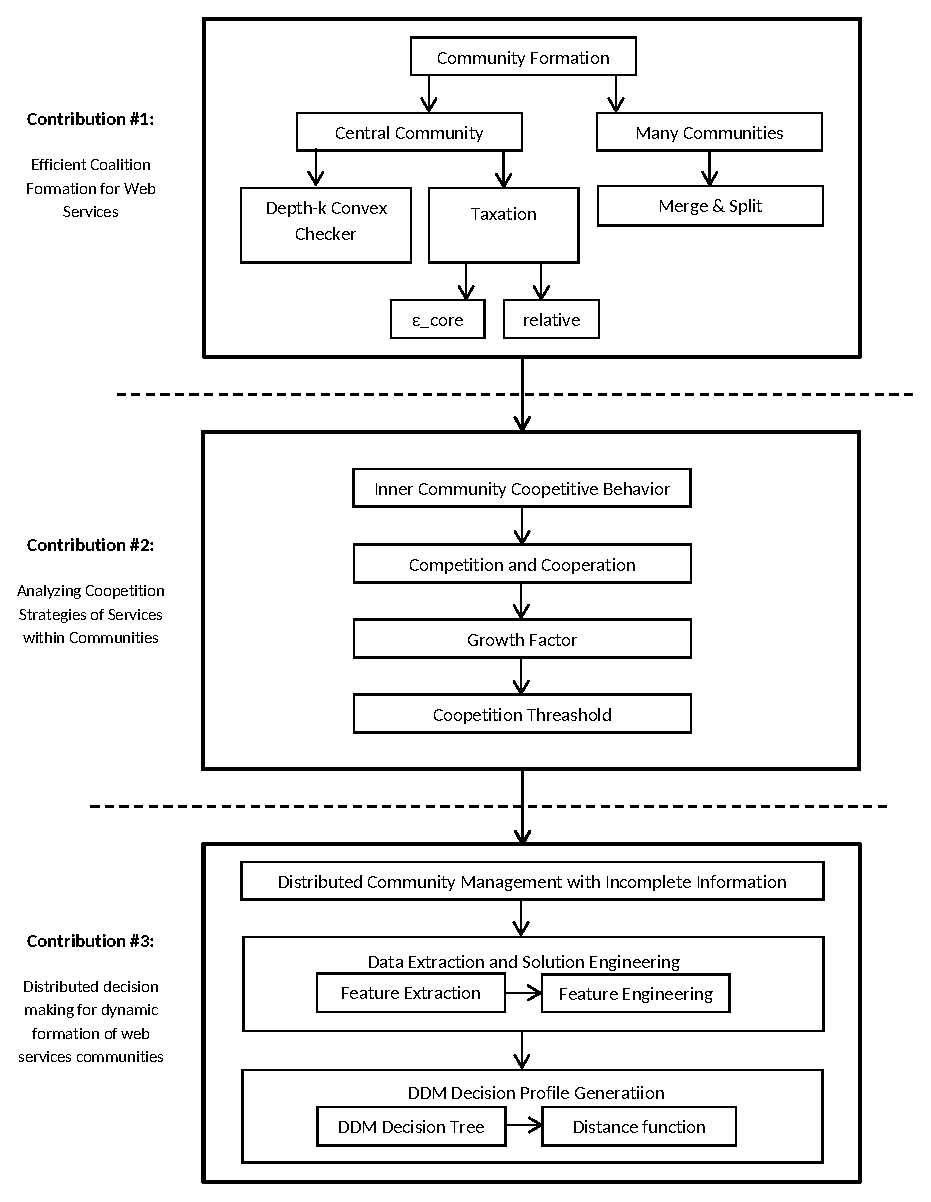
\includegraphics[width=6in]{Figures/structure.eps}`
\caption{The Proposed Framework}
\label{fig_sim1}
\end{figure}

\section{Contributions}\label{sec:in:outline}


\section{Thesis Organization}\label{sec:outline}
The rest of the proposal is organized as follows: We present in
Chapter 111 the background needed for our research along
with relevant related work. Chapter 222
provides the problem statement and presents our solution model in
two different scenarios with some preliminary results. Finally, in
Chapter 333, we present our conclusion,
future plan, and the timetable of our research.



\section{Context of Research}\label{sec:motivation_s}

[seminar] Over the past years, online services have become part of many
scalable business applications. The increasing reliance on
web-based applications has significantly influenced the way web
services are engineered.
%Web services provide a set of stateless
%software functions accessible at a network address over the web.
%The recent developments are shifting web services from passive and
%individual components to autonomous and group-based components
%where interaction, composition, and cooperation are the key
%challenges \cite{ICWS2011-1,SCC2011-1}. The main objective is to
%achieve a seamless integration of business processes, applications
%and web services. Delivering high quality services considering the
%dynamic and unpredictable nature of the Internet is still a very
%critical and challenging issue.
%Typically, web services are business applications deployed as
%autonomous and interoperable agents \cite{Alescio}. In fact, the
%W3C consortium defines a web service as ``an abstract notion that
%must be implemented by a concrete agent''. However, the web is
%stocked with agent-based services that offer similar business
%functionalities, which leads to service consumers having
%difficulties in choosing the most appropriate agents to interact
%with.
The need for highly available and responsive services has called
for grouping and collaborative mechanisms of loosely-coupled web
services, particularly in business settings. The idea of grouping
web services within communities and the way those communities are
engineered so that web services can better collaborate have been
proposed and investigated in
\cite{DBLP:journals/ijebr/MaamarSTBB09,DBLP:journals/internet/BenatallahSD03,Rosario:2008:PQS:1512146.1512290}.
Communities are virtual groups of web services having similar
functionalities \cite{Zeng:2003:QDW:775152.775211,
Paik:2005:TSS:2229263.2230038,Medjahed05adynamic,10.1109/ARES.2008.7},
but probably different non-functional quality attributes, which
form the QoS parameters.
%When communities are used, users send
%their requests to the masters of those communities, which are
%responsible of managing the communities, forwarding the requests
%to the suitable member web services and checking the credentials
%of those members.
Communities aim to provide higher service
availability and performance than what individual web services can
provide.
%The high availability of services and the community
%resilience to failure are guaranteed since web services can
%cooperate and replace each other within the same community and
%since there is no single point of failure in the communities
%architecture.


\section{Motivation and Research Objectives}\label{sec:motexample_s}

Web service communities are dynamic by design
\cite{DBLP:journals/ijebr/MaamarSTBB09}. In these communities, web
services are modeled as intelligent autonomous agents, where they
can adopt a strategy maximizing their payoff at any time. A web
service can ask joining a community and has the right to leave it.
Community managers can invite or ask a web service to leave in
order to maximize the community profit. Users can simply stop
sending requests to a web service which is not providing
satisfactory services. Thus it is important to consider all the
parties involved in the decision making process about the
community management.

In this research work, our first objective is to propose a
cooperative model as game for the aggregation of web services
within communities. The solution concepts of our cooperative game
seeks to find efficient ways of forming coalitions (teams) of web
services so that they can maximize their gain and payoff, and
distribute the gain in a fair way among all the member services.
Achieving Fairness when the gain is distributed among the
community members is the main factor to keep the coalition stable
as no web service will expect to gain better by deviating from the
community. In other words, the coalition is made efficient if all
the members are satisfied. We first propose a representation
function for communities of web services based on their QoS
attributes. By using this function, we can evaluate the $worth$ of
each community of web services. When facing new membership
requests, a typical community master checks whether the new
coalition having the old and new set of web services will keep the
community stable or not. The community master will reject the
membership requests if it finds out that the new coalition would
be unstable, preventing $any$ subset of web services from gaining
significantly more by deviating from the community and joining
other communities or forming new ones. The computation of
solutions for cooperative games is combinatorial in nature and
proven to be NP-complete \cite{Algorithmic}, making this
computation impractical in real world applications. However, using
the concepts of coalition stability, the second objective is to
investigate approximation algorithms running in polynomial time
providing web services and community masters with applicable and
near-optimal decision making mechanisms.

Within communities, services can exhibit competitive behavior as they provide the same functionalities and the number of users requests is finite.
However, for the same reason of being functionally similar, services can cooperate with each other, for example to substitute each other in order to perform some sub-tasks.
So as an extension of our work, we have proposed a framework in which services can opt for performing tasks if they feel they are capable enough
or decide to cooperate by showing the availability to perform some sub-tasks.

%We have implemented an online learning mechanism for services with different capabilities to learn over time which strategy to choose based on their own and other services status and capabilities. After establishing states of our model and observing convincing results from our learning method, we plan to extend the learning process using reinforcement learning (Q-learning) techniques.



\indent To summarize, the main problems we aim to tackle in this
thesis are the formation of stable and efficient coalitions
maximizing web services and community revenue and the decision over the strategy to play about competing or cooperating.
The main objectives are:
\begin{itemize}
\item To propose a cooperative model and analyze its solution
concepts in order to address the problem of optimizing coalition
formation for a stable community.

\item To reduce the complexity of computing the solution concepts
of the cooperative model tailored to the problem of communities of
agent-based web services in order to make these solutions
applicable in real world scenarios.

\item To analyze the effect of different membership and taxation
models that the master can apply to the members on the stability
of the community.

\item To investigate the impact of learning on individual and
group decision making within the cooperative model of the
community.

\item To validate the proposed methods by extensive simulations
and comparison with other similar proposals.
\end{itemize}




\section{Thesis Organization}\label{sec:outline_s}
The rest of the thesis is organized as follows. We present in
Chapter 111 the background needed for our research along
with relevant related work. Chapter 222
provides the problem statement and presents our solution model in
two different scenarios with some preliminary results. Finally, in
Chapter 333, we present our conclusion,
future plan, and the timetable of our research.






%%%%%%%%%%%%%%%%%%%%%%%%%%%%%%%%%%%%%%%%%%%%%%%%%%%%%%%%%%%%%%%%%%%%%%%%%%%%%%%
%% Chapter 2 : Background.
%%%%%%%%%%%%%%%%%%%%%%%%%%%%%%%%%%%%%%%%%%%%%%%%%%%%%%%%%%%%%%%%%%%%%%%%%%%%%%%
\setcounter{chapter}{1}

\chapter{Background}\label{cha:background}
In this chapter, we briefly review web services, then we introduce
the concept of communities of web services, their architecture and
applications and the benefits of forming communities. Thereafter,
we discuss the cooperative game theory concepts used throughout
the proposal. Finally, we discuss relevant related work on web
service communities and games in the literature of service
oriented computing.

\section{Community of Web Services}\label{sec:CommunityWS}
In this section, we present web services and discuss the concept
of their communities from architectural and operations
perspectives.

\subsection{Web Services}\label{sec:CWSWebServices}
Over the past years, online services have become part of standard
daily life of people around the globe. Many modern applications
rely on web services from different providers. For instance, many
mobile and tablet applications which have limited storage and
processing power are merely interfaces aggregating different
information from online services. Examples are vast, weather
forecasting, ticket selling, shopping apps, local maps and places
searching.

The World Wide Web Consortium (W3C) defines web services as
follows: ``software system designed to support interpretable
machine-to-machine interaction over a network. It has an interface
described in a machine-processable format (specifically WSDL).
Other systems interact with the web service in a manner prescribed
by its description using SOAP messages, typically conveyed using
HTTP with XML serialization in conjunction with other Web-related
standards''. When developers declare a new web service, it will be
discovered based on its description that fully discloses its
functionalities. Developers also have to declare a public
interface and a readable documentation to help other developers
when integrating different services \cite{w3cwsdl}. Nowadays, web
API standards which do not require XML-based web service protocols
like SOAP and WSDL are also emerging. They are also called REST
(representational state transfer) services which are moving
towards simpler communication protocols. %They are not restricted
%to XML formats, recently JSON, a human readable and simpler format
%is becoming popular among online service providers.

We are not going to delve into engineering details of online web
service implementation and its protocols in this proposal. We are
interested in web services from their business model perspective.
Service providers usually charge end users for services they
provide. For example, Google has listed their pricing and plans
for wide range of services they provide on their web service
console page\footnote{https://code.google.com/apis/console}.

In our research work, we abstract web services as rational
agents\footnote{The term
        rational is used here in the sense that web services are utility
        maximizers} providing services to end users. They aim to maximize
        their individual income by receiving enough requests from end
        users. In order to increase their revenue, web services seek for
        more tasks if they have the capacity and throughput to do so. Web
        services can join communities to have better efficiency by
        collaborating with others, to have access to broad market share,
        and to have opportunity of receiving a bigger task pool from end
        users. Furthermore, the high reliance on web services has increased quality expectations from end users.
        Communities of web services can provide higher availability, performance, reliability, and recovery for end users.

\subsection{Web Service Communities}\label{sec:CWSDefinition}
Community refers to ``the condition of sharing or having certain
attitudes and interests in common'' or ``a group of people living
in the same place or having a particular characteristic in
common''\footnote{Oxford Dictionaries}. In
\cite{DBLP:journals/internet/BenatallahSD03,
Zeng:2003:QDW:775152.775211}, the authors introduce community of
web services as collection of cooperative web services with common
functionalitiers but different QoS metrics. Therefore
$communities$ are differentiated from $composition$ types of web
service cooperation in which web services with different
functionalities work together to generate a new service with
composite functionality.


Maamar et al. initially in \cite{conf/webist/MaamarLBTS07} and
then comprehensively in \cite{DBLP:journals/ijebr/MaamarSTBB09}
proposed an architecture utilizing \emph{Contract-Net} protocol
for engineering task distribution within communities. This
architecture has been further developed in
\cite{conf/IEEEscc/BenharrefSBB11, conf/IEEEscc/KhosravifarBMMT10,
conf/aina/LimTM11, CSTintercommunity}. Two types of roles have
been distinguished for community members: masters and slaves.
Master web services lead communities and are responsible for
membership management. They can invite and convince slave web
services to join the community, and attract new slave web services
to their communities by awarding them better payoff. Moreover,
they can eject some slave members from the community to improve
its overall reputation if these members are misbehaving or cannot
provide the promised QoS \cite{DBLP:journals/ijebr/MaamarSTBB09}.

        \begin{figure}
            \begin{center}
%            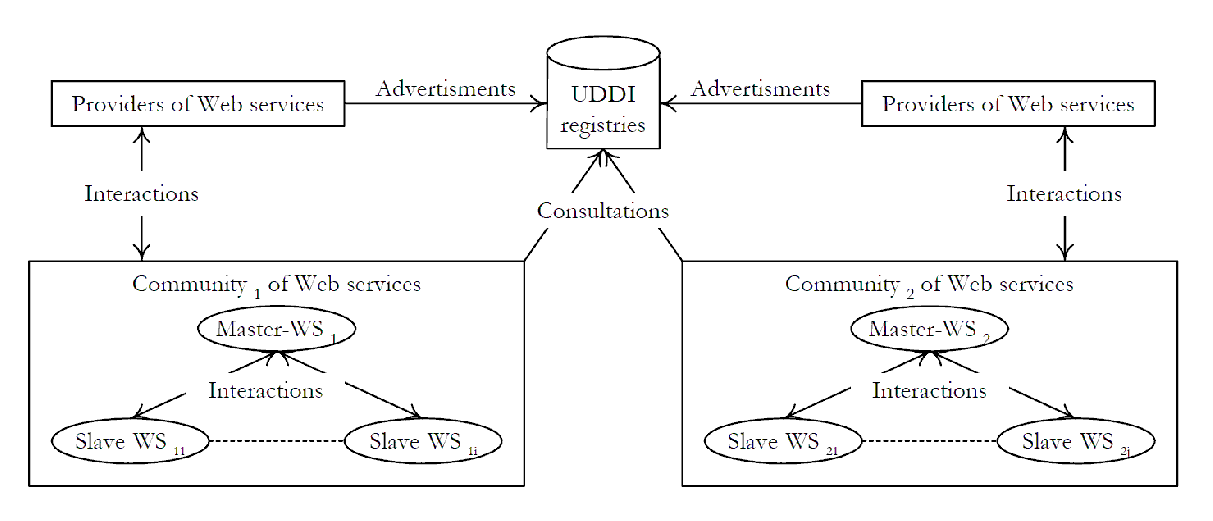
\includegraphics[width=16cm]{Figures/wsarch.eps}\label{wsarch}
            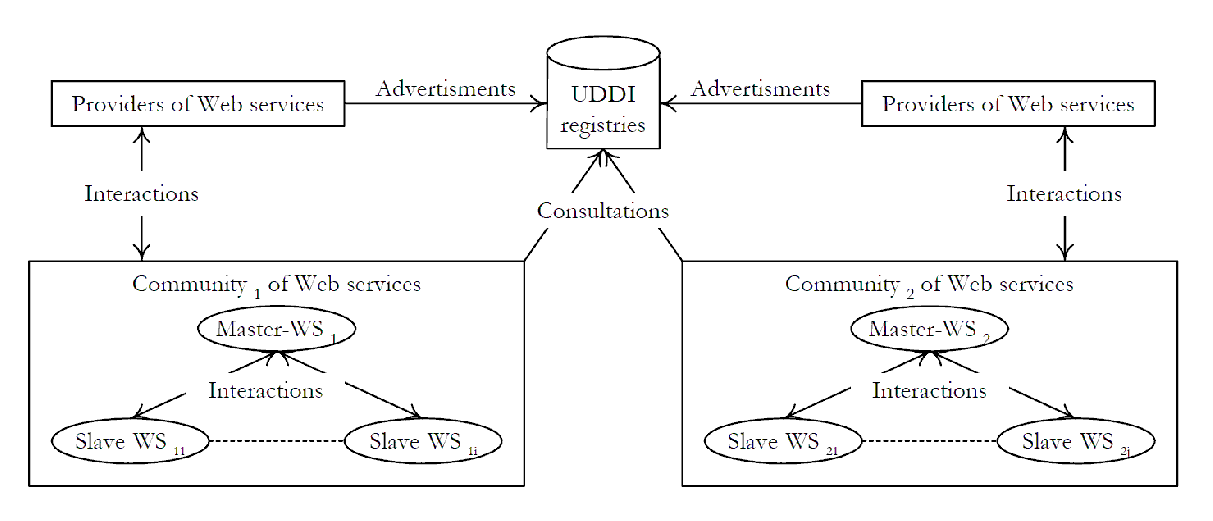
\includegraphics[width=16cm]{Figures/wsarch.eps}\label{wsarch}
            \caption{Communities of Web Services Architecture as Proposed in \cite{DBLP:journals/ijebr/MaamarSTBB09}}
            \end{center}
        \end{figure}

Figure 1 %\ref{wsarch}
depicts the basic architecture of
communities of web services. The main components of the
architecture are: 1) the providers of web services; 2) UDDI
registries; and 3) communities platform. Communities abstract the
same model of defining, announcing and invoking web services. They
also adopt the same protocols that standard web services use with
UDDI registries. UDDI is a platform-independent XML based registry
list which facilitates worldwide web service discovery.

%The master web service is responsible with communication with web
%service providers and discovery registries. It it responsible for
%task distribution, web service selection, community management,
%maintaining a healthy set of web services satisfying end users
%requests with high QoS. In communities, the masters web services
%can be dedicated web services playing the master role during the
%entire time of being in the community. This master web service is
%independently developed and never participates in any
%composition. The master web services can also be chosen out of
%normal web services already inside the community
%\cite{DBLP:journals/ijebr/MaamarSTBB09}.


\section{Cooperative Game Theory and Multi-Agent Systems}\label{sec:CGTMS}

%        Cooperative game theory provides a set of mathematical and optimization tools for multi-agent environments. These tools have been utilized in communication networks and service oriented computing literature, where nodes as rational agents try to reason strategically and maximise their benefit.

Cooperative game is a branch of game theory that studies
strategies of self-interested entities or agents in a setting
where those agents can increase their payoff by binding agreements
and cooperating in groups. We let $N$ be a set of players which
can form a group called a $coalition$. A \emph{coalitional game}
is a pair $G = (N, v)$, where $v$ is called a \emph{characteristic
function} $v: 2^N \to \mathbb{R}$, mapping the set of players of
the coalition to a real number $v(N)$, the worth of $N$. This
number usually represents the output or payoff or again the
performance of these players working together as coalition. If a
coalition $S$ is formed, then it can divide its worth, $v(N)$ in
any possible way among its members. The payoff vector $x \in
\mathbb{R}^N$ is the amount of payoff being distributed among the
members of the coalition $N$. The payoff vector satisfies two
conditions:

        \begin{itemize}
            \item $x_i \geq 0$ for all $i \in N$, and
            \item $\sum_{i \in N} x_i \leq v(N)$
        \end{itemize}

        The second criteria is called the \emph{feasibility} condition,
        according to which, the payoff for each agent cannot be more than
        the coalition total gain. A payoff vector is also \emph{efficient}
        if the payoff obtained by a coalition is distributed amongst the
        coalition members: $\sum_{i \in N} x_i = v(N)$. This definition of
        the characteristic function works in \emph{transferable utility}
        (TU) settings, where utility (i.e., payoff) is transferable from
        one player to another, or in other words, players have common
        currency and a unit of income that is worth the same for all players
        \cite{myerson1991game}.

        When dealing with cooperative games, two issues need to be
        addressed:\\ 1. Which coalitions among all possible coalitions to form? \\
        2. How to reward each member when a task is completed?\\
        %
        The following sections help address these two issues.

        \subsection{Cooperative Game Concepts}


            {\bf Definition 1 (Shapley value)} Given a cooperative game $(N,
            v)$, the \emph{Shapley value} of player $i$ is given by \cite{shapley_value}:
            \begin{equation}\label{eq:shapley}
            \phi_i(N,v) = \sum_{S \subseteq N \backslash \left\{i\right\} }
            \frac{|S|! (|N|-|S|-1)!}{|N|!} (v(S \cup \left\{i\right\}) - v(S))
            \end{equation}

            \emph{Shapley value} is a unique and fair solution concept for
            payoff distribution among the members of the coalition. It
            basically rewards members with the amount of marginal contribution
            they have to the coalition.  It checks the contribution of member $i$ by adding the agent, to all possible subsets
            of coalitions $S$, where $S \subseteq N\backslash\left\{i\right\}$. If he is added to the set $S$, his
            contribution to the coalition is $v(S \cup \left\{i\right\}) - v(S)$. Average marginal contribution of agent $i$'s
            is calculated by averaging this value over all possible subsets of $N$, in $Shapley value$ equation (\ref{eq:shapley}).

            %\subsubsection{Core}

            {\bf Definition 2 (Core)} A payoff vector $x$ is in the $core$ of
            a coalitional game $(N, v)$ if and only if:
            \begin{equation}\label{eq:core}
            \forall S \subseteq N, \sum_{x_i \in S} x_i \geq v(S)
            \end{equation}

            The core is basically a set of payoff vectors where no subset of
            players $S^\prime$ could gain more than their current payoff by
            deviating and making their own coalition $\sum_{i \in S^\prime}
            x_i \geq v(S^\prime)$. The sum of payoffs of the players in any
            sub-coalition $S$ is at least as large as the amount that these
            players could earn by forming a coalition by their own. In a
            sense, it is analogue to Nash equilibrium, except that core is
            about deviations from groups of entities. The core is the
            strongest and most popular solution concept in cooperative game
            theory. However, its computation is a combinatorial problem and
            becomes intractable as the number of players increases. The core
            of some real-world problem games may be empty, which means having
            the characteristic function of the game $(N,v)$, there might be no
            possible distribution of payoff assuring stability of subgroups.

            {\bf Definition 3 (Convex cooperative games)} A game $(N,v)$ with
            characteristic function $v(S)$ is convex if:
            \begin{equation}\label{eq:convex}
            v(S) + v(T) \leq v(S \cup T) + v (S \cap T), \forall S,T \subseteq
            N.
            \end{equation}

            According to a classic result by Shapley \cite{S1971cores}, convex
            games always have a non-empty core. We will use a variation of
            convexity condition in our algorithm to check whether our
            coalitions are stable.

            \subsubsection*{$\epsilon$-core}\label{s:epsilon}
            %\emph{$\epsilon$-Core:}
            %\\
            When the \emph{core} set of a game is empty, it means no coalition
            of players can gain anything by deviating. An outcome would be
            unstable if a coalition can benefit even by a small amount from
            deviating, which is a strong requirement. In fact, in some
            situations, deviations can be costly, or players may have loyalty
            to their coalitions, or even it can be computationally intractable
            to find those small benefits. It would only make sense for a
            coalition to deviate if the gain from a deviation exceeds the cost
            of performing the deviation. \emph{$\epsilon$-core} relaxes the
            notion of the core, and only requires that no coalition would
            benefit significantly, or within a constant amount($\epsilon$) by
            deviating (see Equation \ref{eq:core}).

            \begin{equation}\label{eq:core2}
            \forall S \subseteq N, \sum_{x_i \in S} x_i \geq v(S) - \epsilon
            \end{equation}

            \subsubsection*{Coalition Structure Formation}\label{sec:coalition}

            Coalition structure formation is the problem of finding the best
            partition of web services into teams. In these settings, the
            performance of an individual service is less important than the
            \emph{social welfare} of the whole system, which is the sum of the
            values of all teams. Having the game $(N,v)$, a coalition
            structure $(CS)$ is \emph{socially optimal} if $CS$ belongs to set
            $\operatorname*{arg\,max}_{CS} v(CS)$ where $v(CS)$ is the sum of
            the values of all coalitions inside $CS$. $v(CS) = \sum_{C \in
            CS}v(C)$.
            %The outcome of a characteristic function game in coalition structure settings, consists of two parts; first a disjoint partition of players (agents) into coalitions, called a \emph{coalition structure} (CS) and second a \emph{payoff vector} as mentioned in cooperative game solution concepts, which distributes the value of each coalition among its members.


        %\subsection{Examples on Cooperative Game Solution Concepts}\label{sec:CWSDefinition}

\begin{example}\label{ex:simplecore1}
Consider a game $G = (N, v)$, with two players where $N = {1,2}$.
Each of these players can produce 5 units of output working alone
and by collaborating they can produce 20 units worth of output.
Therefore we have: $v({1}) = 5, v({2}) = 5, v({1,2}) = 20$. The
$core$ of the game, which is the set of all possible distribution
of gain among players guaranteeing stability is: $core(N,v) =
\{(x_1,x_2) \in R^2 | x_1 >= 5, x_2 >= 5, x_1 + x_2 = 20\}$, as
illustrated in Figure 2. Distributing the 20 units of income,
among these two players, for all the points in the line will make
outcome stable, since non of these players can gain more than 5 by
working alone. However although they have same qualities, the core
can suggest a stable outcode where one agent can earn three times
more than the other agent: $\{5,15\}$. As mentioned in previous
section, $core$ result may not be fair, the $core$ only considers
stability. However, \emph{Shapley value} considers fairness.
According to equation \ref{eq:shapley}, the two  workers should
each share 10 units of income, since they have the same marginal
contribution to all subsets of the coalition. As you can see the
distribution vector of $\{10,10\}$ is also a member in $core$ set.
Later we are going to show if $core$ of a coalition game is not
empty, and game is convex, the shapely value lies within $core$
set.
\end{example}

            \begin{figure}
                \begin{center}
                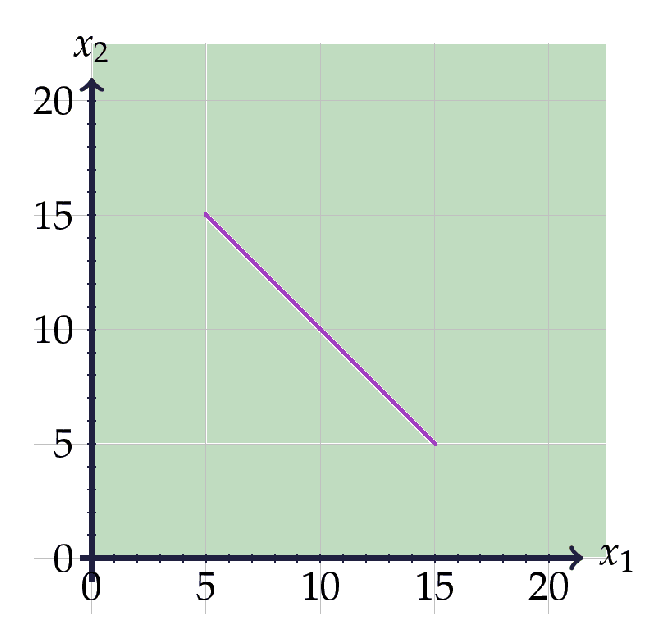
\includegraphics[width=3in]{Figures/excore.eps}\label{fig:coreex1}
                \caption{Core of the 2-player game of example \ref{ex:simplecore1}}
                \end{center}
            \end{figure}


            \begin{example}\label{ex:simplecorealpha}
                In this example, we want to analyse games under conditions which core can be empty. Consider a game $G = (N, v)$,  where $N = {1,2,3}$ and $v(\{i\}) = 0$, $v(\{Ci\}) = \alpha for |C| = 2$ and $v(\{N\}) = 1$. The $(x_1,x_2,x_3)$ distribution vector according to equation \ref{eq:core}, is in $core$ if $x_i \geq 0$ which implies each player will get more than 0 which they would when working alone and $\forall i, \forall j, x_i + x_j \geq \alpha $ which implied any pair of players will get more than $\alpha$ which they would earn if they worked in pair without the third player and finally $\sum_{i \in N} x_i = 1$ which implied all the gain is distributed among the three players. Based on these three equations we have, $\forall i \in N 0 \leqslant 1 - \alpha$ and $\sum_{i \in N} x_i = 1$. By summing first equation for all three platers, we conclude $Core (N,v)$ is nonempty iff $\alpha \leqslant \frac{2}{3}$. When alpha is more than $\frac{2}{3}$, the contribution of third player is not good enough to justify the group of three players working together. The third player will increase the revenue with less then $\frac{1}{3}$, and the other two players, both can get better share of revenue if they work together. This is why the group of three players working together when $\alpha > \frac{2}{3}$ is not stable.
            \end{example}

            %\begin{example}\label{ex:simplecore2}
%
%                An example which has closely resembles our community service model is the \emph{Single landowner and landless workers} example.
%                This example was introduced in \cite{GVK369342747} and represents the \emph{landowner} entity which is providing jobs and \emph{landless workers} who cannot do anything by themselves and need to work with a landowner to gain revenue (payoff).
%
%                In this game, land is owned by a single person, the \emph{landowner}. We refer to the other people as \emph{workers}. In this case we have a game there the set of players are the landowner and the $m$ workers, possible actions for coalitions with only workers would be distributing the zero output for all where no member receives any output. The set of actions of a coalition $S$ consisting of the landowner and $k$ workers would be the set of all $S$-allocations of the output $f(k+1)$ among the members of $S$. The preference of each player would be the amount of out she obtains.
%
%                In this game the action $a_{N}$ of the grand coalition in which the landowner obtains all the output $f$(n)
%                is in the core: all coalitions that can produce any output include the landowner, and none of these
%                coalitions has any actions that makes her better off than she is in $a_{N}$.
%
%                For any value of n The core contains actions in which the workers receive some output.
%                The workers need the landowner to produce any output, but the landowner
%                also needs the workers to produce more than $f$(1), so stable actions of the grand coalition exist in which the
%                workers receive some output. Take the landowner to be player 1, and consider the action $a_{N}$ of the grand
%                coalition in which each player $i$ obtains the output $x_{i}$, where $x_{1}+...+x_{n}=f(n)$. Under what conditions
%                on  $(x_{1},..,x_{n})$ is $a_{N}$ in the core? Because of my assumption about the shape of the function $f$, the
%                coalitions most capable of profitably deviating from $a_{N}$ consist of the landowner and every worker but one.
%                Such a coalition can, by itself, produce $f(n-1)$, and it may distribute this output in any way among its members.
%                Thus for a deviation by such a coalition not to be profitable, the sum of $x_{i}$ and any collection of $(n-2)$ other
%                $x'_{i}$s must be at least $f(n-1)$. That is, $(x_{1}+...+x_{n})-x_{i}\geq f(n-1)$ for every $j=2,..,n$. Because
%                $x_{1}+...+x_{n}=f(n)$, we conclude that $x_{i}\leq f(n)-f(n-1)$ for every player $j$ with $J\geq 2$ (i.e. every worker).
%                That is, if $a_{N}$ is in the core then $0\leq x_{j}\leq f(n)-f(n-1)$ for every player $J\geq 2$. In fact, every such action
%                is in the core, as you are asked to verify in the following exercise.
%
%            \end{example}

%          Core of landowner-worker game: Check that no coalition can improve upon any action of the grand
%          coalition in which the output received by every worker is nonnegative and at most $f(n)-f(n-1)$. (Use the fact that
%          the form of $f$ implies that $f(n)-f(k)\geq (n-k)(f(n)-f(n-1))$ for every $k\leq n$.)

%          We conclude that the core of the game is the set of all actions of the grand coalition in which the output $x_{i}$
%          obtained by each worker $i$ satisfies $0\leq x-{1}\leq f(n)-f(n-1)$ and the output obtained by the landowner is the
%          difference between $f(n)$ and the sum of the worker's shares. In economics jargon, $f(n)-f(n-1)$ is a worker's
%          ``marginal product". Thus in any action in the core, each worker obtains at most her marginal product.

%          The worker's shares of output are driven down to at most $f(n)-f(n-1)$ by competition between coalitions consisting
%          of the landowner and workers, in cahoots with the landowner, can deviate and increase their share of output. That is,
%          each worker's share of output is limited by her comrade's attempts to obtain more output.

%          The fact that each worker's share of output is held down by interworker competition suggests that the workers might
%          be better off if they were to agree not to join deviating coalitions \emph{except as a group}. You are  asked to check
%          this idea in the following exercise.

        %\subsection{Cooperative Games in Service Oriented Computing}\label{sec:CWSArchitecture}

        \subsection{Representation and Complexity Issues}\label{sec:CWSArchitecture}

        Shapely value is the unique ``fair'' way to distribute the total surplus generated by the coalition, among all the players.
        The nature of the Shapley value is combinatorial, as all possible orderings to form a
        coalition needs to be considered. This computational complexity can sometimes be
        an advantage as agents cannot benefit from manipulation. For example, it is NP-complete
        to determine whether for a bunch of agents to collude and make their own coalition and guarantee
        an increase in payoff of all participants \cite{conf/aaai/YokooCSOI05}.
        There are some representations that allow us to compute the Shapley value efficiently by reducing the input size of the problem.
        One example is \emph{Induced subgraph games}
        which was introduced by Deng and Papadimitriou \cite{Deng94}. In this representation, players are represented by graph nodes, and
        their valuation function should be the sum of weights of all edges between the node and all its neighbors. It is a succinct representation, using
        an adjacency matrix, which needs only $O(n^2)$ space to store all the input, which is a major improvement from $O(2^n)$ because
        if weights of all the edges in graph are all positive, the Shapley value can be computed in time $O(n^2)$.
        However, this representation is not complete, some games cannot be represented by a induced subgraph game \cite{conf/aaai/YokooCSOI05}.

        Ketchpel introduces the Bilateral Shapley Value (BSV) \cite{conf/aaai/Ketchpel94a} for coalition games with general valaution functions.
        It reduces the combinatorial complexity of the computation of the Shapley value, breaking the community to multiple disjoint set.
        With backtracking and dynamic programming like methods, they merge and store the marginal contribution of disjoint coalitions,
        reducing the overall complexity of the algorithm. However, the solution is still NP-Complete and BSV time and space complexity grows exponentially.

        In order to make cooperative game concepts practical in real world application, we have proposed an approximation multi-layer
        algorithm useful for service orinted computing settings. Our excrements illustrate, these algorithms can provide
        applicable and near optimal solutions for real world applications.


\section{Related Work}\label{sec:BRRelatedWork}

The idea of grouping web services within virtual structures was
fist proposed by Zeng et al. \cite{Zeng:2003:QDW:775152.775211}.
The authors defined web service community as collection of web
services providing the same functionality, but with different
quality metrics. Medjahed and Boubuettaya
\cite{journals/dpd/MedjahedB05} have proposed a framework and a
community builder mechanism which uses semantic analysis,
providing an ontological organization of web services having the
same domain of interest. The community builder would suggest web
services having similar operations to join the same community, or
form their own community in case the semantic analysis cannot find
any community that matches the service types.

        Most of the recent work on communities of services are either
        user-centric and focus on user satisfaction
        \cite{Chun02user-centricperformance} or system-centric and focus
        on the whole system throughput, performance and utilization. There
        are many contributions in distributed, grid, cluster and cloud
        services which are system-centric. However, in real world
        environments and applications, both users and service providers
        are self-interested agents, aiming to maximize their own profit.
        In those environments, both parties (users and services) will
        collaborate as long as they are getting more benefits and payoff.

        In this direction, recently \cite{DBLP:conf/IEEEscc/LimTMB12,
        DBLP:conf/IEEEscc/KhosravifarABT11, 10.1109/TSC.2012.12} proposed mechanisms to help
        users and services maximize their gain. A two-player
        non-cooperative game between web services and community master was
        introduced in \cite{DBLP:conf/IEEEscc/KhosravifarABT11}. In this
        game-theoretic model, the strategies available to a web service
        when facing a new community are requesting to join the community,
        accepting the master's invitation to join the community, or
        refusing the invitation to join. The set of strategies for
        communities are inviting the web service or refusing the web
        service's join request. Based on their capacity, market share and
        reputation, the two players have different set of utilities over
        the strategy profiles of the game. The main limits of this game
        model are: 1) its consideration of only three quality parameters,
        while the other factors are simply ignored; and 2) the
        non-consideration of the web services already residing within the
        community. The game is only between the community master and the
        new web service, and the inputs from all the other members are
        simply ignored. The consideration of those inputs is a significant
        issue as existing web services can lose utility or payoff because
        of the new member, which can results in an unhealthy and unstable
        group. The problem comes from the fact that the existing members
        should collaborate with the new web services, so probably their
        performance as a group can suffer. Existing members may even
        deviate and try to join other communities if they are unsatisfied.
        Those considerations of forming stable and efficient coalitions
        are the main contributions of this research work.

        In \cite{DBLP:conf/IEEEscc/LimTMB12}, a 3-way satisfaction approach
        for selecting web services has been proposed. In this approach,
        the authors proposed a web service selection process that the
        community masters can use. The approach considers the efficiency
        of all the three involved parties, namely users, web services and
        communities. In this work, it is shown how the gains of these
        parties are coupled together using a linear optimization process.
        However, the optimization problem in this solution tends to
        optimize some parameters considering all web services regardless
        of their efficiency and contribution to the community's welfare.
        Moreover, there are no clear thresholds for accepting or rejecting
        new web services. The solution of the optimization problem could,
        for instance, suggest web services already residing within the
        community to increase or decrease their capacity to cover up the
        weakness of other parties in the system. However, a high
        performing web service could deviate anytime it finds itself
        unsatisfied within the community instead of adjusting its service
        parameters.

        In \cite{10.1109/TSC.2012.12}, a cooperative scheme among autonomous
        web services based on coalitional game theory has been introduced. The authors have proposed an algorithm to
        reach individually stable coalition partition for web services in order to
        maximize their efficiency. The communities choose new web services on the promise
        that it would benefit the community without decreasing any other web service's
        income. In their model, the worth of community is evaluated with high emphasis on
        availability metric and considering price and cost values only. The community structure is based on a coordination chain,
        where a web service is assigned as a \emph{primary} web service and the community task destribution
        method, will initially invoke the primary web service and only if the primary web service is unavailable
        will invoke the next backup web services as they are ordered in the coordination chain. However in cooperative models, it is preferred to
        have a real and active cooperative activity engaging all agents to perform the tasks more efficiently. Especially nowadays
        with recent advancement in cloud and hardware infrastructures availability is becoming less of an issue. So the backup web services
        in their model have a very low chance of getting jobs, especially the ones further in chain, which is huge waste of web services
        capabilities.

\section{Conclusive Remarks}


        In this research work, we will use game theory to
        propose a cooperative game model for the aggregation of web
        services within communities. The solution concepts of our
        cooperative game seeks to find efficient ways of forming
        coalitions (teams) of web services so that they can maximize their
        gain and payoff, and distribute the gain in a fair way among all
        the web services. Achieving Fairness when the gain is distributed
        among the community members is the main factor to keep the
        coalition stable as no web service will expect to gain better by
        deviating from the community. In other words, the coalition is made
        efficient if all the members are satisfied. We first propose a
        representation function for communities of web services based on
        their QoS attributes. By using this function, we can evaluate the
        $worth$ of each community of web services. When facing new
        membership requests, a typical community master checks whether the
        new coalition having the old and new set of web services will keep
        the community stable or not. The community master will reject the
        membership requests if it finds out that the new coalition would
        be unstable, preventing $any$ subset of web services from gaining
        significantly more by deviating from the community and joining
        other communities or forming new ones. The computation of
        solutions for cooperative game theory problems is combinatorial in
        nature and proven to be NP-complete \cite{Algorithmic}, making
        this computation impractical in real world applications. However,
        using the concepts of coalition stability, we propose
        approximation algorithms running in polynomial time providing web
        services and community masters with applicable and near-optimal
        decision making mechanisms.


%%%%%%%%%%%%%%%%%%%%%%%%%%%%%%%%%%%%%%%%%%%%%%%%%%%%%%%%%%%%%%%%%%%%%%%%%%%%%%%
%% Chapter 3 : Probabilistic Social Commitments.
%%%%%%%%%%%%%%%%%%%%%%%%%%%%%%%%%%%%%%%%%%%%%%%%%%%%%%%%%%%%%%%%%%%%%%%%%%%%%%%
\setcounter{chapter}{2}


\chapter{Coalition Formation for Autonomous Web Services}\label{sec:coalitionformationws}

In this chapter, we present our coalition model of agent-based web
services within communities \cite{SCC2013efficient}. We start by describing the general
architecture and considered parameters for web services.
Thereafter, problem modeling and formulation will be introduced in
terms of task distribution and community revenue. Web service
cooperative games in different settings will follow along with
some simulation results.

\section{Preliminaries}\label{s:preliminaries}

In this section, we discuss the parameters and preliminary
concepts that we use in the rest of the proposal.

\subsection{Architecture}

Our system consists of three main types of entities working
together:

\emph{1) Web services} are rational entities that aim to maximize
their utilities by providing high quality services to end users.
They aim to maximize their individual income by receiving enough
requests from end users. In order to increase their revenue, web
services seek for more tasks if they have the capacity and
throughput to do so. Web services can join communities to have
better efficiency by collaborating with others, to have access to
higher market share, and to have opportunity of receiving a bigger
task pool from end users. Throughout this proposal, in our
equations, we refer to web services as $ws$ and to the set of web
services hosted by a given community as $C$. To simplify the
notation, sometimes we simply write $ws$ instead of $ws \in C$ to
go through the elements $ws$ of the set $C$.

\emph{2) Master Web Services} or the community coordinators, are representatives of the
communities of web services and responsible for their management.
Communities receive requests from users and aim to host a healthy
set of web services to perform the required tasks. They seek to
maximize user satisfaction by having tasks accomplished according
to the desired QoS. In fact, higher user satisfaction will bring
more user requests and increase the market share and revenue of
the community.

\emph{3) Users} generate requests and try to find the best
available services. User satisfaction is abstracted as function of
quantity and quality of tasks accomplished by a given service.
Higher user satisfaction leads to higher trust of the community by users hence directing more requests towards that service provider.

\subsection{Web Service Parameters}\label{ws_parameters}

Web services come with different quality of service parameters.
These parameters with a short description are listed in Table
\ref{qosws}.

\begin{table}[!t]
\centering
\caption{List of web service QoS parameters.}
\begin{tabular}{|c|c||c|c|}
\hline
\textbf{Parameter} & \textbf{Definition} \\
\hline\hline
$Availability$ & Probability of being available during \\
&a time frame \\
$Reliability$ & Probability of successfully handling \\
&requests during a timeframe\\
$Successability$ & Rate of successfully handled requests \\
$Throughput$ & Average rate of handling requests \\
$Latency$ & The average latency of services\\
$Capacity$ & Amount of resources available\\
$Cost$ & Mean service fee \\
$Regulatory$ & Compliance with standards, law and rules\\
$Security$ & Quality of confidentiality \\
&and non-repudiation\\
\hline
\end{tabular}
\label{qosws}
\end{table}


We adopted a real world dataset \cite{DBLP:conf/smc/Al-MasriM09a}
which has aggregated and normalized each of these parameters to a
real value between 0 and 1. Since requests are not shared among
web services and are distributed among all of them inside a
community, each one of them comes with a given QoS denoted by
$(QoS_{ws})$. We assume that $(QoS_{ws})$ is obtained by a certain
aggregation function of the parameters considered in Table
\ref{qosws}. We use this quality output later in evaluating the
community \emph{worth} or \emph{payoff} function.

\subsection{Web Service Communities}\label{webservice-communities}

Figure 3 represents our revised architecture of web service
communities where tasks are to be distributed among the members
that are interested in forming stable coalitions. As discussed in
Chapter 2, communities are essentially virtual platforms
aggregating web services having similar and complementary
functionalities and communicate with other entities such as UDDI
registries and users using particular protocols. Web services join
communities to increase their utility by having larger market
share and task pool. Community coordinators or master web services
are responsible for community development, managing membership
requests from web services and distributing user tasks among the
community members. Community coordinators try to attract quality
web services and keep the community as stable and productive as
possible to gain better reputation and user satisfaction, which
results in having higher revenue.

\begin{figure*}[!t]
\centerline{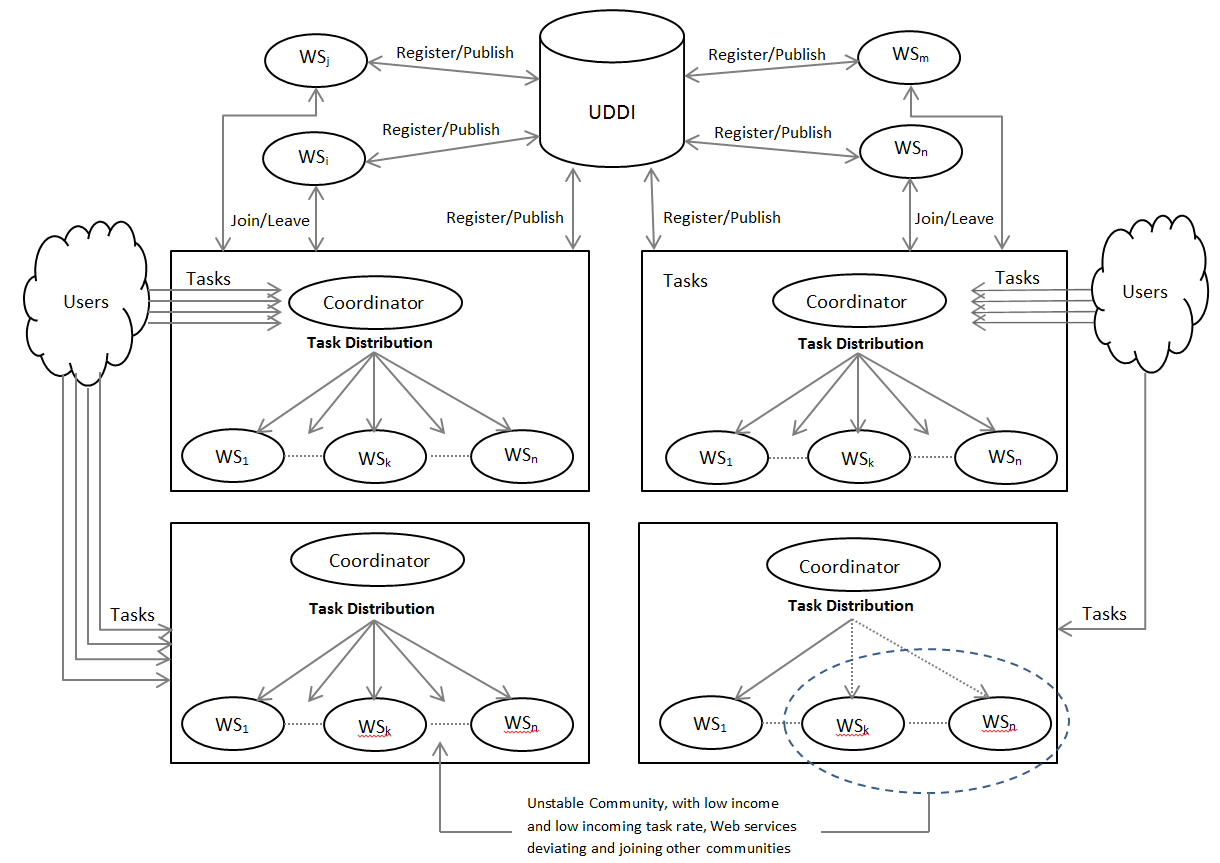
\includegraphics[width=15cm]{Figures/archss.eps}}
\caption{Architecture of Web Service communities}
\label{fig_community}
\end{figure*}


\section{Problem Formulation and Modeling}\label{s:model}

In this section, we present  web services and community coordinator's interactions, the task distribution process and revenue models in web service communities.

\subsection{Task Distribution}

As mentioned in Section \ref{s:preliminaries}, communities
are robust service providers with well established market share
and reputation. By maintaining their reputation and performance,
they attract  end users which choose them as service providers to
perform their tasks. The community master is characterized by a
request rate $(R_C)$ from users. Each web service comes with a
given QoS ($QoS_{ws}$) from which the throughput $Th_{ws}$ is
excluded. Throughput is the average rate of tasks a web service
can perform per time unit. Its exclusion from $QoS_{ws}$ allows us
to build our analysis on the particular value of $Th_{ws}$. Thus,
web services perform tasks with an average output quality of
$QoS_{ws}$ and a throughput rate of $Th_{ws}$.

The community master uses a slightly modified \emph{weighted fair queuing} method to distribute tasks among its members. The goal is to allocate incoming tasks to web services with a rate matching the throughput value of $Th_{ws}$. In \emph{weighted fair queuing} method \emph{all} the input flow is multiplexed along different paths, however in our case if the input rate $(R_C)$ of the community is more than the summation of throughput values of the web services in the community, some of the input tasks will be queued and served with delay. Thus, the amount of tasks performed by community is $\sum_{ws \in C}{(Th_{ws})}$ when $\sum_{ws}{Th_{ws}} \leq R_{C}$. However, when the input rate $(R_C)$ of the community is less than the summation of throughput values of the web services in the community,
%the community has more web services having more total throughput value than community's request rate
$(R_C)$ the \emph{weighted fair queuing} algorithm assigns a weighted task rate of $R_C \times \frac{Th_{ws}}{\sum_{ws}{Th_{ws}}}$ for each web service ($ws$) and the total rate of tasks being performed is $R_C$, the community's receiving request rate.

While distributing tasks, the community master can verify the performance, throughput and quality of service of   tasks being performed by web services. It can recognize if web services are capable of doing the amount of tasks they advertised. If for any reason there is a decline in quality metrics or throughput, the  community master will announce the new parameters and community masters and members can consider those values as benchmark for future performance calculations.
Web services that got their quality declined are penalized, and in this way, players have incentive to reveal their real capabilities to profit best from the community and to avoid being penalized. In addition, the system should be dynamic enough to detect and react to web services quality metrics variation as over time web service metrics may  degrade or improve, a change that the community should adjust to.
% Therefore its easy for the system to encourage players to be in some sense incentive compatible in the way that they would profit best by truthfully revealing their capabilities. Also it is important to be dynamic enough to consider web services which may have their quality metrics degraded or even improved over time for any reason and be able to adjust the community with new parameters.


\subsection{Community Revenue}

The communities and web services earn revenue by performing tasks.
The total gain is function of quality ($QoS_{ws}$) and throughput
($Th_{ws}$) of tasks being performed. We have adopted a linear equal weight average over
the QoS parameters excluding the
$Throughput$ and $Cost$ parameters. A community has the option to
weigh specific QoS parameters depending on the expectations of
their clients.

The maximum potential output of a community $(PO(C))$  is an aggregation of number of tasks, times their quality, for each web service member of the community:

\begin{equation}
PO(C) = \sum_{ws \in C}{(T_{ws} \times QoS_{ws})}
\end{equation}

If the summation of throughput values ($Th_{ws}$) of community members exceeds the input task rate of the community ($R_C$) the community cannot perform at its maximum potential. It denotes the case when the community has more web services than it needs to perform the input task load. The actual output has to be normalized to the amount of tasks being performed.

\begin{equation}\label{out_c}
Out(C) = \left\{
  \begin{array}{l l}
    PO(C) & \quad \text{if $\sum_{ws}{Th_{ws}} \leq R_{C}$}\\
    PO(C) \times \frac{R_{C}}{\sum_{ws}{Th_{ws}}} & \quad \text{if $\sum_{ws}{Th_{ws}} > R_{C}$}
  \end{array} \right.
\end{equation}

The revenue function of the web service community is a linear function of $Out(C)$ with a positive constant multiplier.

\subsection{Case Study}

In this section, we analyze three numerical examples and discuss the motivation of web services and community interactions and the strategies they can adopt and the revenue they can earn adopting these different strategies.


%%%%%%%%%%%%%%%%%%%%%%%%% EXAMPLE 1 %%%%%%%%%%%%%%%%%%%%%%%%%%%%%%%%%%%%
\begin{table}[!t]
\renewcommand{\arraystretch}{1.3}
% if using array.sty, it might be a good idea to tweak the value of
% \extrarowheight as needed to properly center the text within the cells
\caption{Case Study: Example 1}
\label{example_1}
\centering
\begin{tabular}{c c c c}
\hline
$WS$ & $QoS_{ws}$ & $Th_{ws}$ & $Th_{ws} \times QoS_{ws}$\\
\hline
1 & 0.8 & 4 & 3.2\\
2 & 0.8 & 5 & 4.0\\
3 & 0.8 & 3 & 2.4\\
\hline
\end{tabular}
\end{table}

\begin{table}[!t]
\renewcommand{\arraystretch}{1.3}
% if using array.sty, it might be a good idea to tweak the value of
% \extrarowheight as needed to properly center the text within the cells
% \caption{Three web services}
\label{example_1_2}
\centering
\begin{tabular}{c c || c c}
\hline
Community & Worth & Community & Worth\\
\hline
$\left\{1\right\}$ & 3.2 & $\left\{1,2\right\}$ & 7.2\\
$\left\{2\right\}$ & 4.0 & $\left\{1,3\right\}$ & 5.6\\
$\left\{3\right\}$ & 2.4 & $\left\{2,3\right\}$ & 6.4\\
$\left\{1,2,3\right\}$ & 8.0\\
\hline
Community $R_C$: 10\\
\hline
\end{tabular}
\end{table}
%%%%%%%%%%%%%%%%%%%%%%%%% EXAMPLE 1 %%%%%%%%%%%%%%%%%%%%%%%%%%%%%%%%%%%%

%%%%%%%%%%%%%%%%%%%%%%%%% EXAMPLE 2 %%%%%%%%%%%%%%%%%%%%%%%%%%%%%%%%%%%%
\begin{table}[!t]
\renewcommand{\arraystretch}{1.3}
% if using array.sty, it might be a good idea to tweak the value of
% \extrarowheight as needed to properly center the text within the cells
\caption{Case Study: Example 2}
\label{example_2}
\centering
\begin{tabular}{c c c c}
\hline
$WS$ & $QoS_{ws}$ & $Th_{ws}$ & $Th_{ws} \times QoS_{ws}$\\
\hline
1 & 0.8 & 5 & 4.0\\
2 & 0.7 & 6 & 4.2\\
3 & 0.7 & 4 & 2.8\\
\hline
\end{tabular}
\end{table}

\begin{table}[!t]
\renewcommand{\arraystretch}{1.3}
% if using array.sty, it might be a good idea to tweak the value of
% \extrarowheight as needed to properly center the text within the cells
% \caption{Three web services}
\label{example_2_2}
\centering
\begin{tabular}{c c || c c}
\hline
Community & Worth & Community & Worth\\
\hline
$\left\{1\right\}$ & 4.0 & $\left\{1,2\right\}$ & 7.4\\
$\left\{2\right\}$ & 4.2 & $\left\{1,3\right\}$ & 6.8\\
$\left\{3\right\}$ & 2.8 & $\left\{2,3\right\}$ & 7.0\\
$\left\{1,2,3\right\}$ & 7.3\\
\hline
Community $R_C$: 10\\
\hline
\end{tabular}
\end{table}
%%%%%%%%%%%%%%%%%%%%%%%%% EXAMPLE 2 %%%%%%%%%%%%%%, %%%%%%%%%%%%%%%%%%%%%%

In the first example,  we present the case of a community with
$R_C =10 $, and three web services, each having different
$QoS_{ws}$ and $Th_{ws}$ values as listed in Table
\ref{example_1}. The worth of a community is calculated based on
$Out(C)$ equation (\ref{out_c}) which is the amount of output
being generated by the community. The first table  lists the web
services with their aggregated $QoS_{ws}$ parameters, their task
input rate while working alone, and also their  throughput value
$Th_{ws}$. The second table shows all the possible communities and
their respective worth. The obtained values suggest that
communities having more web services have better gain and output.
However each community needs to  distribute the gain between web
services. Sometimes it is impossible to share the gain between all
web services in a way that no subset of them would individually
gain more if they form their own group. In this example, the value
community of ${ws_1}$ and ${ws_2}$ is 7.2, With ${ws_3}$ joining
the community the worth increases to 8.0. However there is no way
to distribute the value among web services to have  ${ws_1}$ and
${ws_2}$  earning 7.2, and ${ws_3}$ earning at least 2.4, the gain
they could earn before joining the community. This fact makes the
group unstable. In the second  example, shown in Table
\ref{example_2}, we even have situations where a web service
(${ws_3}$) joining a community ($\left\{ws_1,ws_2\right\}$)
decreases the value of community. The reason is, the community is
already full and all tasks are almost being distributed and new
community with bad quality can degrade the average quality of
tasks being done by the community. In both examples, the request
of joining of web service ${ws_3}$ should be rejected by the
community.

%%%%%%%%%%%%%%%%%%%%%%%%% EXAMPLE 3 %%%%%%%%%%%%%%%%%%%%%%%%%%%%%%%%%%%%
\begin{table}[!t]
\renewcommand{\arraystretch}{1.3}
% if using array.sty, it might be a good idea to tweak the value of
% \extrarowheight as needed to properly center the text within the cells
\caption{Case Study: Example 3}
\label{example_3}
\centering
\begin{tabular}{c c c c}
\hline
$WS$ & $QoS_{ws}$ & $Th_{ws}$ & $\text{\emph{Input Task Rate}}$\\
\hline
1 & 0.8 & 10 & 5\\
2 & 0.8 & 20 & 5\\
3 & 0.8 & 30 & 5\\
\hline
\end{tabular}
\end{table}

\begin{table}[!t]
\renewcommand{\arraystretch}{1.3}
% if using array.sty, it might be a good idea to tweak the value of
% \extrarowheight as needed to properly center the text within the cells
% \caption{Three web services}
\label{example_3_2}
\centering
\begin{tabular}{c c || c c}
\hline
Community & Worth & Community & Worth\\
\hline
$\left\{C_{ms_1}\right\}$ & 0 & $\left\{C_{ms_2}\right\}$ & 0\\
$\left\{C_{ms_1}, ws_1\right\}$ & 8 & $\left\{C_{ms_2}, ws_1\right\}$ & 8\\
$\left\{C_{ms_1}, ws_2\right\}$ & 16 & $\left\{C_{ms_2}, ws_2\right\}$ & 16\\
$\left\{C_{ms_1}, ws_3\right\}$ & 16 & $\left\{C_{ms_2}, ws_3\right\}$ & 24\\
$\left\{C_{ms_1}, ws_1, ws_2\right\}$ & 16 & $\left\{C_{ms_2}, ws_1, ws_2\right\}$ & 24\\
$\left\{C_{ms_1}, ws_1, ws_3\right\}$ & 16 & $\left\{C_{ms_2}, ws_1, ws_3\right\}$ & 32\\
$\left\{C_{ms_1}, ws_2, ws_3\right\}$ & 16 & $\left\{C_{ms_2}, ws_2, ws_3\right\}$ & 32\\
$\left\{C_{ms_1}, ws_1, ws_2, ws_3\right\}$ & 16 & $\left\{C_{ms_2}, ws_1, ws_2, ws_3\right\}$ & 32\\
$\left\{C_{ms_1}, C_{ms_2}, ...\right\}$ & 0 & $\left\{ws_1\right\}$ & 6.8\\
$\left\{ws_2\right\}$ & 4.2 & $\left\{ws_3\right\}$ & 6.8\\
\hline
Community $R_{C_1}$: 20 \\ Community $R_{C_2}$: 40\\
\hline
\end{tabular}
\end{table}
%%%%%%%%%%%%%%%%%%%%%%%%% EXAMPLE 3 %%%%%%%%%%%%%%%%%%%%%%%%%%%%%%%%%%%%

In Example 3, we consider the case of having different communities with different market share, ${R_C}$ values. Web services also have a small share of market independently, providing them with a small task pull. In these kind of scenarios, the solution considers individual maximization of payoff and also the total worth of all communities which represents the \emph{social welfare}. In this example the most efficient partition of web services is earned by having two coalitions of $\left\{C_{master_1}, ws_2\right\}$ and $\left\{C_{master_2}, ws_1, ws_3\right\}$, which yields a total value of $32 + 16 = 48$. In these types of scenarios, the goal is to reach stability, adopting a distributed approach where all players have the power of choice on the decision of whether or not they join a coalition. The communities usually start the game having some established members, encountering new web services, the communities may exchange web services and new web services would join them having at least one player gaining utility, without hurting any other participant. In this example if we initially having two coalitions of $\left\{C_{master_1}, ws_2\right\}$ and $\left\{C_{master_2}, ws_1\right\}$ and a ${ws_3}$ as new web service, ${ws_3}$ joining ${C_{master_1}}$ would hurt at least itself or $ws_2$, however ${ws_3}$ joining ${C_{master_2}}$ would not hurt any participants and ${ws_3}$ would earn more within the community and the community will have enough web services performing the incoming tasks from users.

The first two examples illustrate the fact that a community cannot simply increase its revenue by adding more web services. The web services and even community owners are autonomous agents and would deviate and be displeased about the community if new members cause a drop in their profit. The job of the community master is to attract as many quality web services it can and keep them satisfied; hence the group stability is guaranteed.
The third example highlights another type of problem we would like to address, which is how to form best possible groups of communities, and allocate web services among communities in a way which would maximize payoff for of our agents and members already residing in the communities.
In next section, we provide collaborative game theory based algorithms for our autonomous agents, to tackle these problems and find applicable and efficient strategies for communities and web services to maximize their profit.

 \section{Web Service Cooperative Games}\label{s:game_solution}

In this section, we present different web service community models
and focus on the problem of how both web services and community
masters as rational entities would adopt strategies to maximize
their payoff.

\subsection {Web Services and One Community}

In this scenario, we assume the existence of a typical community
managed by its master, and web services need to join it to be able
to get requests from the master. The community master is
characterized by a requests rate $(R_{C})$ from users. Each web
service comes with a given QoS ($QoS_{ws}$). The worth of a community
$v(C)$ is set to Out(C) based on equation \ref{out_c}.

As mentioned in previous section, the worth and output of a
community  is a function of the
throughput and provided QoS of its web service members. If the throughput rate is more than
the master's input request rate, it means the web services inside
the community are capable of serving more requests than the
demand. Considering this factor, the valuation function is
designed to balance the output performance so that it matches the
exact throughput rate and QoS the web service can provide within
the particular community.
%** In the case where the limited tasks are distributed among web services uniformly, the value of coalition would be the proportion of the average QoS times their throughput to rate of available requests. **

In this first scenario, we only consider one grand coalition and
analyze the system from the point of view of one single master web
service and a collection of web services. The master web service
decides which members can join
%or should leave%
the community and distributes the requests and income among its
community members (see Figure \ref{fig_sim1}).

\begin{figure}[!t]
\centering
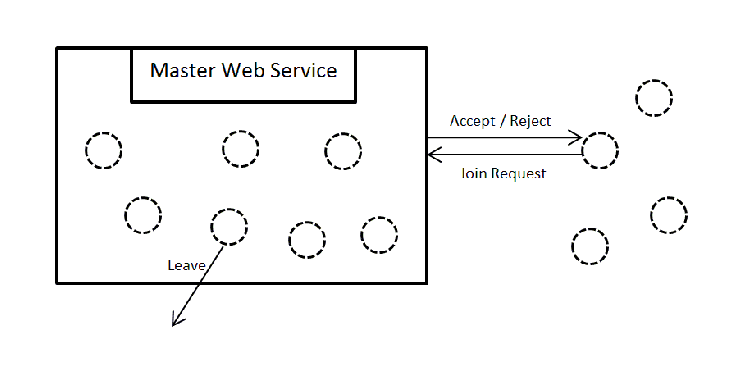
\includegraphics[width=3in]{Figures/s1.eps}`
\caption{Web Services and A Grand Community}
\label{fig_sim1}
\end{figure}

The membership decision is made based on throughput and \emph{QoS}
of the considered web service. The goal is to have quality web
services in the community so it stays stable and no other web
services would have incentives to deviate and leave the coalition
$C$. Therefore, a basic method would be to check the core of the
coalition $C$ considering all the current community members (all
web services already residing within the community) and the new
web service. This algorithm uses the \emph{Shapley value}
distribution method as described in Equation \ref{eq:shapley} to
distribute the gain of $v(C)$ among all the members and then
checks if the \emph{Shapley value} payoff vector for this
community having the characteristic function $v(C)$ is in the
\emph{core}. In the \emph{Shapley value} payoff vector, the payoff
for each web service $ws_i$ is calculated based on its marginal
contribution $v(C \cup {i}) - v(C)$ over all the possible
different permutations in which the coalition can be formed, which
makes the payoff distribution fair. Because of going through all
the possible permutations of subsets of $N$, the nature of the
\emph{Shapley value} is combinatorial, which makes it impractical
to use as the size of our coalitions grows. However, it is proven
that in convex games, the \emph{Shapley value} lies in the core
\cite{DBLP:conf/ijcai/GrecoMPS11, myerson1991game}. Thus, if the
\emph{Core} is non-empty, the payoff vector is a member of the
\emph{Core}. The following proposition is important to make our
algorithm tractable.
% so in our algorithm we check the core membership of this payoff vector.

%\ref{eq:convex}.

%\newtheorem{theorem}{Proposition}
%\begin{theorem}[Einstein-Podolsky-Rosenberg]
\begin{theorem}\label{proposition1}
A game with a characteristic function $v$
is convex if and only if for all $S$, $T$, and $i$ where $S
\subseteq T \subseteq N \backslash \left\{i\right\}, \forall i \in
N$,
%For $\forall S \subseteq T \subseteq N \backslash \left\{i\right\}, \forall i \in N$ we have:
\begin{equation}\label{eq:convex_snow}
v(S \cup \left\{i\right\}) - v(S) \leq v (T \cup \left\{i\right\}) - v(T)
\end{equation}
\end{theorem}

%\begin{Proposition}\label{proposition} A game with a characteristic function $v$
%is convex if and only if for all $S$, $T$, and $i$ where $S
%\subseteq T \subseteq N \backslash \left\{i\right\}, \forall i \in
%N$,
%For $\forall S \subseteq T \subseteq N \backslash \left\{i\right\}, \forall i \in N$ we have:
%\begin{equation}\label{eq:convex_snow}
%v(S \cup \left\{i\right\}) - v(S) \leq v (T \cup \left\{i\right\}) - v(T)
%\end{equation}
%\end{Proposition}

\begin{proof}
We first prove the ``only if'' direction:
%\\$~~~~$\textbf{1}. ``only if'' direction:\\
\\$~~~~$\ \textbf{1}. ``only if'' direction:\\
%\setlength{\abovedisplayshortskip}{2pt}
Assume:\\
\vspace{-0.5cm}
\begin{gather*}\label{convexsnowproof}
v(S \cup \left\{i\right\}) - v(S) \leq v (T \cup \left\{i\right\})
- v(T)
\\
\rightarrow v(S \cup \left\{i\right\}) + v(T) \leq v (T \cup \left\{i\right\}) + v(S)
\end{gather*}

Considering $S \subseteq T$:
\setlength{\abovedisplayshortskip}{2pt}
\begin{gather*}
T \cup \left\{i\right\} = (S \cup \left\{i\right\}) \cup T
\\
S = (S \cup \left\{i\right\}) \cap T
\end{gather*}

By setting $A = S \cup \left\{i\right\}$ and $B = T$ we have:
\setlength{\abovedisplayshortskip}{2pt}
\begin{gather*}
v(S \cup \left\{i\right\}) + v(T) \leq v (T \cup \left\{i\right\}) + v(S)
\\
\rightarrow v(S \cup \left\{i\right\}) + v(T) \leq
\\
v((S \cup \left\{i\right\}) \cup T) + v((S \cup \left\{i\right\}) \cap T)
\\
\rightarrow v(A) + v(B) \leq v(A \cup B) + v(A \cap B)
\end{gather*}
Consequently, the game is convex.

\textbf{2}. ``if'' direction:\\
Assume the game is convex. Thus, for all $A, B \subset N$, we
have: \setlength{\abovedisplayshortskip}{2pt}
\begin{gather*}
v(A) - v(A \cap B) \leq v(A \cup B) - v(B)
\end{gather*}

By setting $S \cup \left\{i\right\} = A$ and $T = B$ where $S \subseteq T$:
\setlength{\abovedisplayshortskip}{2pt}
\begin{gather*}
v(S \cup \left\{i\right\}) - v((S \cup \left\{i\right\}) \cap T) \leq v(T \cup (S \cup \left\{i\right\})) - v(T)
\\
\rightarrow v(S \cup \left\{i\right\}) - v(S) \leq v(T \cup \left\{i\right\}) - v(T)
\end{gather*}

\end{proof}

Thus, in order to keep the characteristic function convex, new web
services should have more marginal contribution as the coalition
size grows.

Our algorithm works as follows. Given an  established community
with a master and some member web services, a web service would send a \emph{join request} to join  the
community. Ideally, the \emph{core}
or \emph{$\epsilon$-core} stability of the group having this new
member should be analyzed. As the normal core membership algorithm is computationally
intractable, we exploit Proposition \ref{proposition1} and Equation
\ref{eq:convex_snow} to check the convexity of our game having
characteristic function where the new member is added. In the
equation, let $C$  be our community members before
having the new web service join the community. Let  ${i}$ be the new web
service, and then verify the equation for $S$, setting $ S = T /
W1 $ where $W1$ is the set of all possible subsets of the set $N$
having the size $1$. We can relax the equation a bit by adding a
constant $\epsilon$ to the left side of the equation. We call this
method \emph{Depth-1 Convex-Checker} algorithm. If the equation is
satisfied for all $W1$, we let the new web service join our
community, since the web service will contribute positively enough
to make our new community stable. Since only subsets of size $1$
are checked, the following Proposition holds.

\begin{theorem}\label{complexity1}
\emph{The run time complexity of Depth-1 Convex-Checker algorithm is
$O(n)$.}
\end{theorem}

By this result, we obtain a significant reduction from $O(2^n)$,
which is the complexity of checking all possible subsets of $N$.
In our second method, we use the same algorithm, but this time we
set $W2$ to be the set of all possible subsets of size two and one
of the community $C$. We call this method \emph{Depth-2
Convex-Checker} and its run time complexity is still
linear:

\begin{theorem}\label{complexity2}
\emph{The run time complexity of Depth-2 Convex-Checker algorithm is
$O(n^2)$.}
\end{theorem}

It is possible to develop an algorithm that continues the
verification of this condition against subsets of size $3$,
$4$, etc. until the algorithm gets interrupted.

\subsection {Web Services and Many Communities}

In this scenario, we consider multiple communities managed by
multiple master web services, each of which is providing
independent request pools (see Figure \ref{fig_sim2}). Identical
to the first scenario, master web services form coalitions with
web services. We use coalition structure formation methods to
partition web services into non-empty disjoint coalition
structures. As mentioned in Section \ref{sec:coalition}, the used
algorithms in \cite{Sandholm:1999:CSG:317145.317152,DBLP:conf/ijcai/GrecoMPS11,DBLP:conf/ijcai/RahwanMJ11} try to
solve key fundamental problems of what coalitions to form, and how
to divide the payoffs among the collaborators.

\begin{figure}[!t]
\centering
\includegraphics[width=3in]{Figures/s2.eps}
\caption{Web Services and Many Communities}
\label{fig_sim2}
\end{figure}

In coalition-formation games, formation of the coalitions is the
most important aspect. The solutions focus on maximizing the
social welfare. For any coalition structure $\pi$, let
$v_{cs}(\pi)$ denote the total worth $\sum_{C \in \pi}{v(C)}$,
which represents the \emph{social welfare}. The solution concepts
in this area deal with finding the maximum value for the social
welfare over all the possible coalition structures $\pi$. There
are $centralized$ algorithms for this end, but these approaches
are generally NP-complete. The reason is that the number of all
possible partitions of the set $N$ grows exponentially with the
number of players in $N$, and the centralized algorithms need to
iterate through all these partitions.
%These algorithms \cite{DBLP:conf/ijcai/GrecoMPS11, DBLP:conf/ijcai/RahwanMJ11, RePEc:wpa:wuwpga:0110001} are centralized algorithms, where all the complexity. However these algorithms are more intractable than Core stable solutions and practical with some constraints in practice\cite{RePEc:wpa:wuwpga:0110001}.
In our model, we propose using a distributed algorithm where each
community master and web service can be a decision maker and
decide for its own good. The aim is to find less complex and
distributed algorithms for forming web services coalitions
\cite{DBLP:journals/igtr/AptW09,Dieckmann02dynamiccoalition,ray2007game}.
The distributed merge-and-split algorithm in
\cite{DBLP:journals/igtr/AptW09} suits our application very well.
It keeps splitting and merging coalitions to partitions which are
preferred by all the players inside those coalitions.

This merge-and-split algorithm is designed to be adaptable to
different applications. One major ingredient to use such an
algorithm is a preference relation or well-defined orders proper
for comparing collections of different coalition partitions of the
same set of players. Having two partition sets of players, namely
$P = {P_1,...,P_k}$ and $Q = {Q_1,...Q_l}$, one example would be
to use the social welfare comparison $\sum^k_{i=1}v(P_i) >
\sum^l_{j=1}v(Q_j)$. For our scenario, we use \emph{Pareto order}
comparison, which is an individual-value order appropriate for our
self-interest web services. In the Pareto order, an allocation or
partition $P$ is preferred over another $Q$ if at least one player
improves its payoff in the new allocation and all the other
players still maintain their payoff ($p_i \geq q_i$ with at least
one element $p_i > q_i$).

The valuation function $v(C)$ for this scenario is the same as
\emph{``Web Services and One Community''} scenario. However, in
order to prevent master web services joining the same community,
we set $v(C) = 0$ when $C$ has either none, or more than one
master web service as member.

In this scenario, as new web services are discovered and get ready
to join communities, our algorithm keeps merging and splitting
partitions based on the preference function. The decision to merge
or split is based on the fact that all players must benefit. The
new web services will merge with communities if $all$ the players
are able to improve their individual payoff, and some web services
may split from old communities, if splitting does not decrease the
payoff of \emph{any} web service of the community. According to
\cite{DBLP:journals/corr/abs-cs-0605132}, this sequence of merging
and splitting will converge to a final partition, where web
services cannot improve their payoff. More details of this
algorithm and analysis of generic solutions on coalition formation
games are described in \cite{DBLP:journals/igtr/AptW09}.

\subsection{Taxation, Subsiding and Community Stability}\label{s:tax}

We discussed $core$ as one of the prominent solution concepts in
cooperative games. Working together, completing tasks and
generating revenue, agents need to distribute the gain in a way no
agents would gain more by forming their own group. However, in
most cases, the core of a game is empty, so we introduced the
\emph{$\epsilon$-core} concept, where agents would only earn a
minimal amount of $\epsilon$ by deviating from the coalition.
Stability is an attractive property for communities. In addition,
communities would benefit by having slightly more web services
than the exact number of web services needed to satisfy the task
rate cap. This is because there is always a possibility that the
web services may leave the community or they may under perform and
degrade the quality values they were initially performing with.

The solution we propose for communities to ensure stability is
applying a tax $\epsilon$, which is an amount of cost for those
web services that decide to change communities (let us say from
$C$ to $C'$), which would make deviation a costly act. However,
this would require all the community coordinators to agree on a
same amount of taxation, being governed by some external entities;
otherwise, web services would join communities charging the lowest
amount of tax. Before deciding to change the community, each web
service $i$ has to be sure that the gain $g_i(C \rightarrow C')$
calculated in Equation \ref{eq:gainsh} based on the Shapley values
of $i$ in the previous and new communities and the tax $\epsilon$
is positive, which means, what the web service would gain in $C'$
is greater than what it gains in $C$ and the tax it would pay if
moving all together:


\begin{equation}\label{eq:gainsh}
g_i(C \rightarrow C') = \phi_i(C',v) - \phi_i(C,v) - \epsilon
\end{equation}


Another viable solution we introduce to our scenario is to
stabilize the game using external subsidies. The reason a game is
not stable is that the community is not making enough revenue to
allocate enough gain to the players. A community coordinator can
subside its community with a constant coefficient value of
$\lambda$.
%
%Rewarding a community with high number of quality participants
%with $\lambda v(C)$, where $\lambda \leq 1$.
%
Obviously, with a big value for $\lambda$, it is always possible
to stabilize the community. However, this can be a costly act for
the community coordinators, so they are interested in the minimum
subside value of $\lambda$ making the community stable. This can
be achieved by solving the following linear program:
%
  \begin{alignat*}{3}
    \min~   & \lambda  \\
    \text{s.t. } & \lambda v(C) > v(C') & ~& \text{ for all } C' \subset C
  \end{alignat*}


%When a new web service $i$, wants to join the community, the
%valuation function of the community members and the new web
%service is subsided by the community coordinator in order to
%incentivize formation of this community and is set to:
%\begin{equation}\label{eq:taxv}
%v'(C \cup \{i\}) = \lambda \times v(C \cup \{i\})
%\end{equation}
%In equation \ref{eq:taxv} the value of $v'$ is
%replaced with the valuation function for the new forming coalition
%$C \cup \{i\}$.
Subsiding or taxing in order to reduce the
bargaining power of sub coalitions are called $taxation$
\cite{eps346856} methods. We evaluate the effectiveness of these
two methods experimentally through extensive implementations in
the next section.



%Thus, another way to garantee \emph{$\epsilon$-core} stability can be achieved by some surplus payments from community coordinators. These concepts of applying cost in coallition values in order to reduce their bargaining power are called $taxtation$ methods\cite{eps346856}.

%The \emph{$\epsilon$-core} concept, in its definition, considers the willing to join or deviate from agent's point of view. It claims agents for any reason will be not willing to deviate to gain less than $\epsilon$ amount of profit. Communities can agree on However, in our case, the community master is willing to keep web services in communities too. There are several reasons for this, one reason is there is always possibility that agents may leave the community or they may under perform from the quality values they were initially performing with. To this end, our communities will reward and valuate web services in the community


\section{Experimental Results and Analysis}\label{s:resutls}


In this section, we discuss the experiments we performed for our
scenarios to validate the applicability and performance of our
proposed methods in realistic environments.
An XML SOAP based messaging system was implemented. We created a pool of web services and populated most of
their \emph{QoS} parameters from a real world web service dataset
\cite{DBLP:conf/smc/Al-MasriM09a}\footnote[1]{The implemented
environment includes the QWS dataset by Eyhab Al-Masri and Qusay
H. Mahmoud freely available at:
http://www.uoguelph.ca/\textasciitilde{}qmahmoud/qws/.}. To test
our methods, we formed around 10,000 random coalitions consisting
of 3 to 160 web services. In average, the communities were populated by 60 web
services. We implemented the
scenarios using Java and executed the experiments on an Intel Xeon
X3450 machine with 6GBs of memory.

One of the key criteria reflecting the performance of web service
coalitions is the user satisfaction. User satisfaction can be
measured in terms of quality and quantity of requests (or tasks)
successfully answered by the communities. We initiated the
communities with few web services, then let rejecting and
accepting random web services go for a short number of iterations.
After that, we started the request distribution for the communities
and let them allocate requests among member web services.
Thereafter, we measured the average output performance of tasks in
communities following different methods.

\begin{figure}[!t]
\centering
%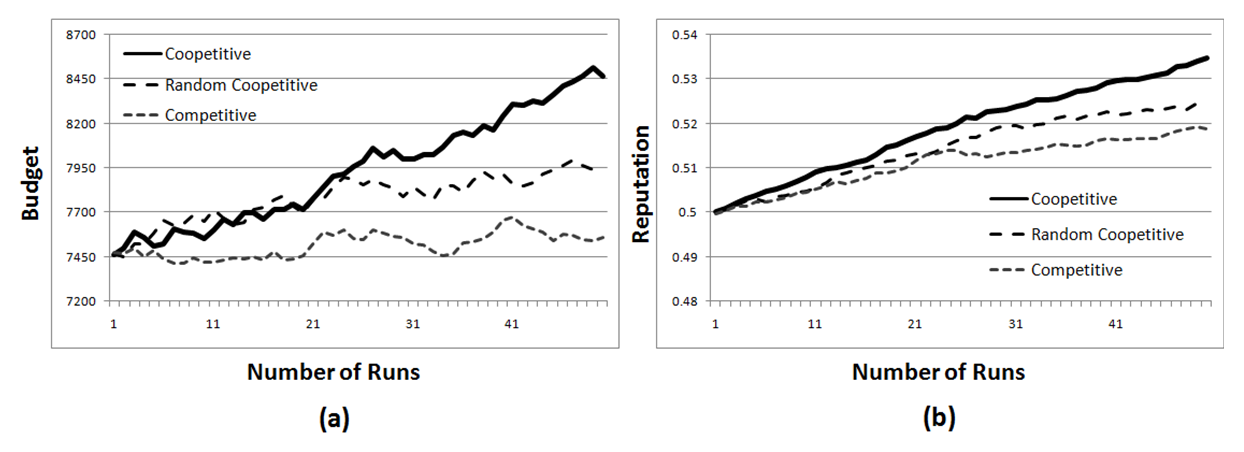
\includegraphics[scale=0.6]{graph1Final+.eps}
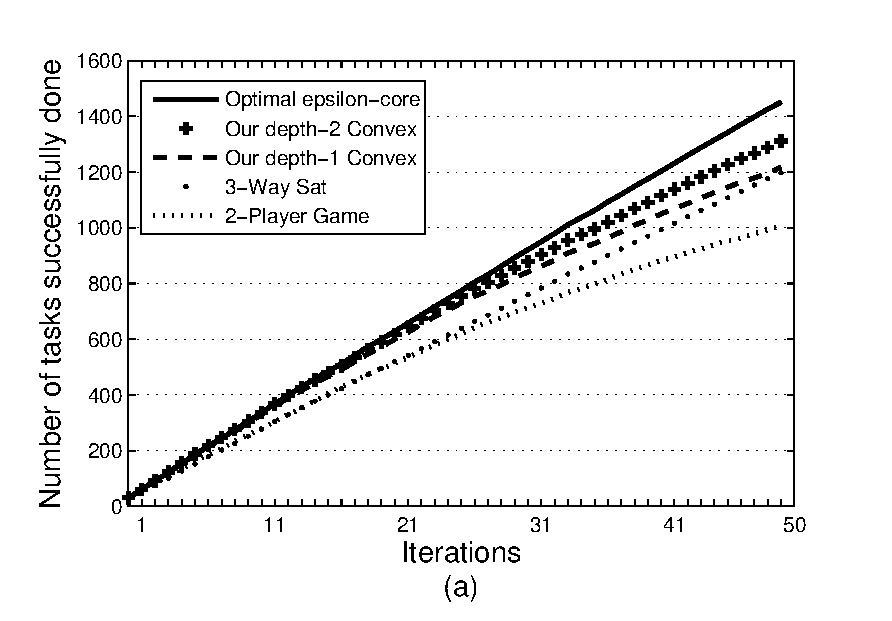
\includegraphics[width=2.8in]{Figures/task_done_opt.eps}
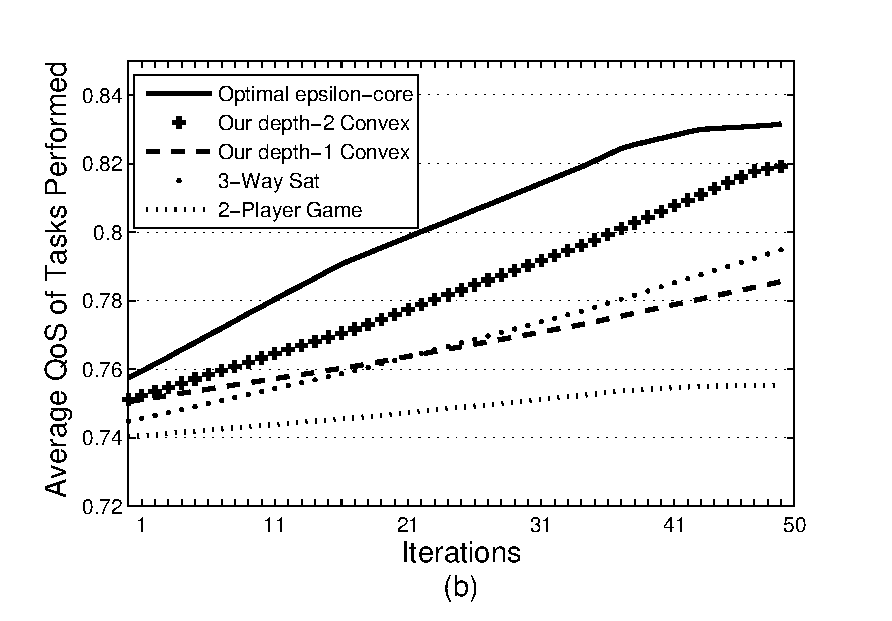
\includegraphics[width=2.8in]{Figures/task_qos_opt.eps}
\caption{Part (a): Cumulative number of requests successfully
done. Part (b): Average QoS of requests performed.}
\label{performanceall}
\end{figure}

Figure \ref{performanceall} depicts the results of optimal
\emph{$\epsilon$-core}, \emph{Depth-1 Convex-Checker},
\emph{Depth-2 Convex-Checker}, \emph{3-Way Satisfaction}
\cite{DBLP:conf/IEEEscc/LimTMB12}, and \emph{2 Player
Non-Cooperative} \cite{DBLP:conf/IEEEscc/KhosravifarABT11} methods
in \emph{one grand community with many web services} scenario.

For the \emph{optimal core} method we have used the well known \emph{$\epsilon$-core} method as the
taxtation method to relax the core condition to help communities, attract web services.
We have assigned $\epsilon$ to 15\% of total community worth, $\epsilon = 0.15 \times v(C)$, which allows
subsets of the coalition to gain maximum 15\% of $v(C)$. In the
\emph{optimal $\epsilon$-core} method, we capped the coalition
size to 25 web services, since the method is computationally
intractable as number of web services increase and anything more than that would make it
impractical to run in our simulations. In the other methods, there
were no cap on size of the community and we had communities of
size 60 web services at some points. In this scenario our community receives 30 tasks on average per iteration, from users. The community, after the task distribution process on each iteration, will reevaluate QoS metrics of its members and can check for new membership requests. Web services may join or leave the community between iterations. The results show that our
\emph{depth-2 convex checker} method is performing better compared
to the other methods and its performance is close to optimal
\emph{$\epsilon$-core} method. Our \emph{depth-1 convex checker}
and the \emph{3-Way Satisfaction} method, are also performing well.

\begin{figure}[!t]
\centering
%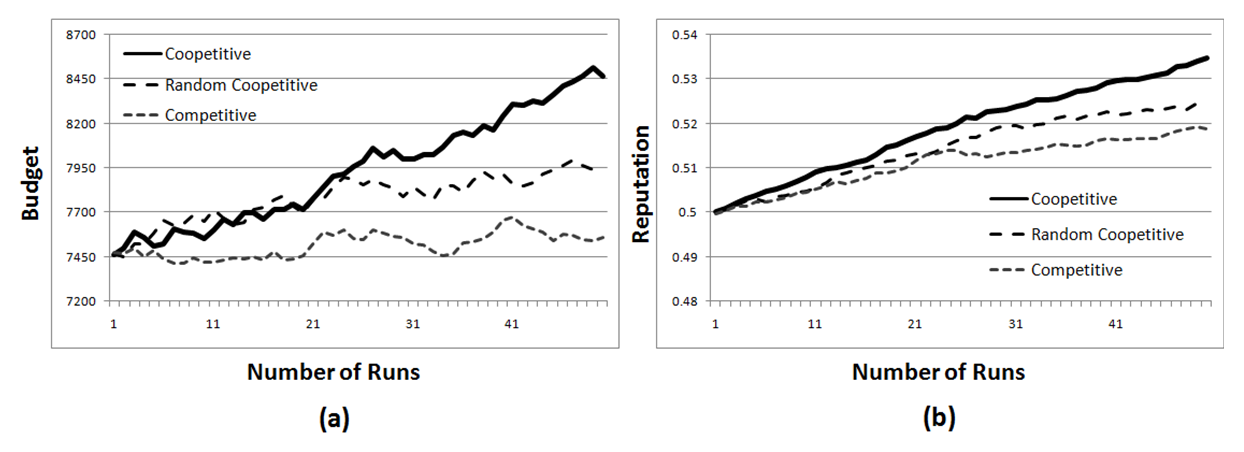
\includegraphics[scale=0.6]{graph1Final+.eps}
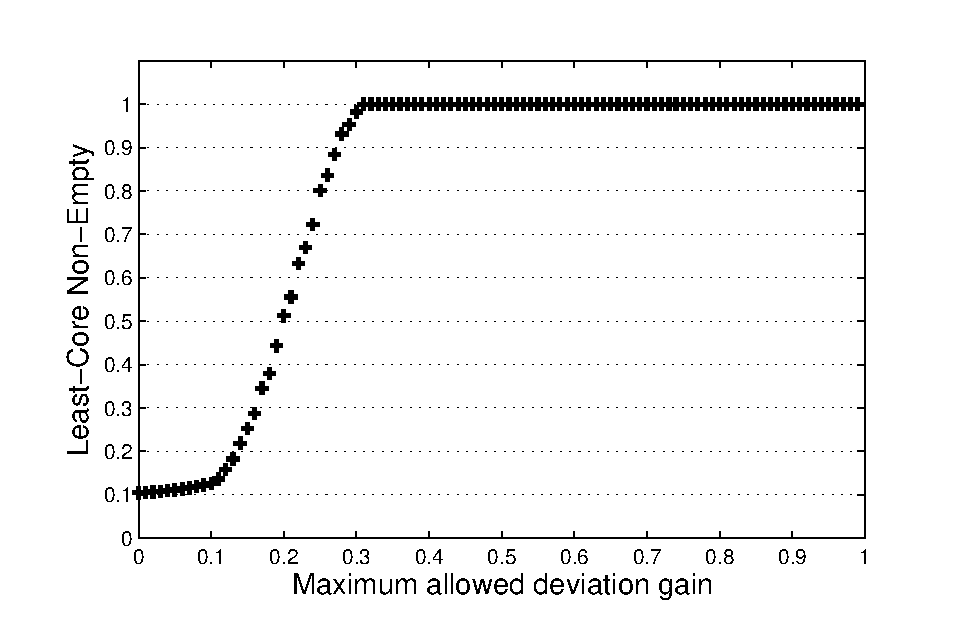
\includegraphics[width=3in]{Figures/least_core.eps}
\caption{Analysis of \emph{$\epsilon$-core} set non-emptiness, for different values of $\epsilon$} \label{f_leastcore}
\end{figure}

As mentioned in Section \ref{s:preliminaries}, the concept of
\emph{core}, assumes no coalition of players can gain anything by
deviating, which is a fairly strong requirement, and that is why
the notion of \emph{$\epsilon$-core} was introduced. Least-Core
$e(G)$ of a game $G$, is the minimum amount of $\epsilon$ so that
the core is not empty. We evaluated the non-emptiness of \emph{$\epsilon$-core} set using the
valuation function and a set of web services. We picked random
number of web services from the dataset and formed around 10,000
random coalitions consisting of 3 to 26 web services. We choose 26
as the maximum number of members in our coalition since it
is computationally very complex for larger coalitions to verify whether
\emph{$\epsilon$-core} set is empty or not. Also instead of considering $\epsilon$ amount of constant deviation in \emph{$\epsilon$-core} definition (Equation \ref{eq:core2}), we similarly defined \emph{relative $\epsilon$-core} concept where no coalition would benefit more than \emph{$\epsilon$ $\times$ v(C)} by deviating. We set $\epsilon$ between 0 and 1 and verify the \emph{relative $\epsilon$-core} set non-emptiness. The results in Figure
\ref{f_leastcore} illustrates that almost 10\% of our random web
service coalitions have non-empty \emph{core} solution and
\emph{$\epsilon$-core} solution is \emph{always} non-empty when we
let agents gain only 30\% more of $v(C)$ by deviating.

One of the properties of coalition structure formation algorithms
in our second scenario is that they partition web services with low
throughput rate so that they usually join coalitions with less
request rate. Since the characteristic function $v(C)$ and the
fair Shapely payoff vector is proportional to web services'
contribution, the web services with small contribution will get
paid much less in communities having web services with high
throughput. On the other hand, according to the valuation function
$v(C)$, web services with high throughput will not contribute well
to communities with low amount of user requests (low market
share). The strong web services are likely to deviate from weak
coalitions, joining a stronger one, which makes the initial
coalition unstable.


\begin{figure}[!t]
\centering
%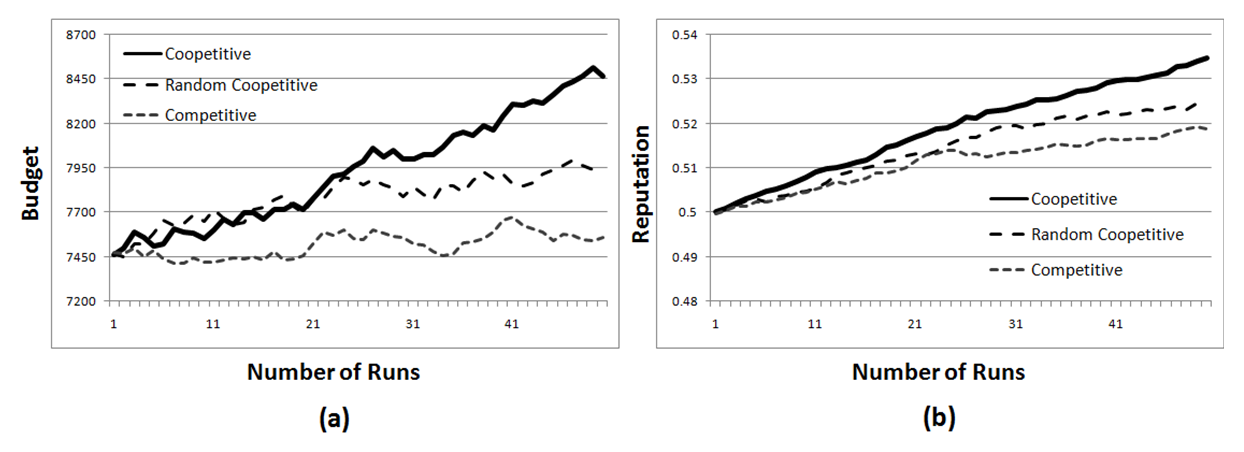
\includegraphics[scale=0.6]{graph1Final+.eps}
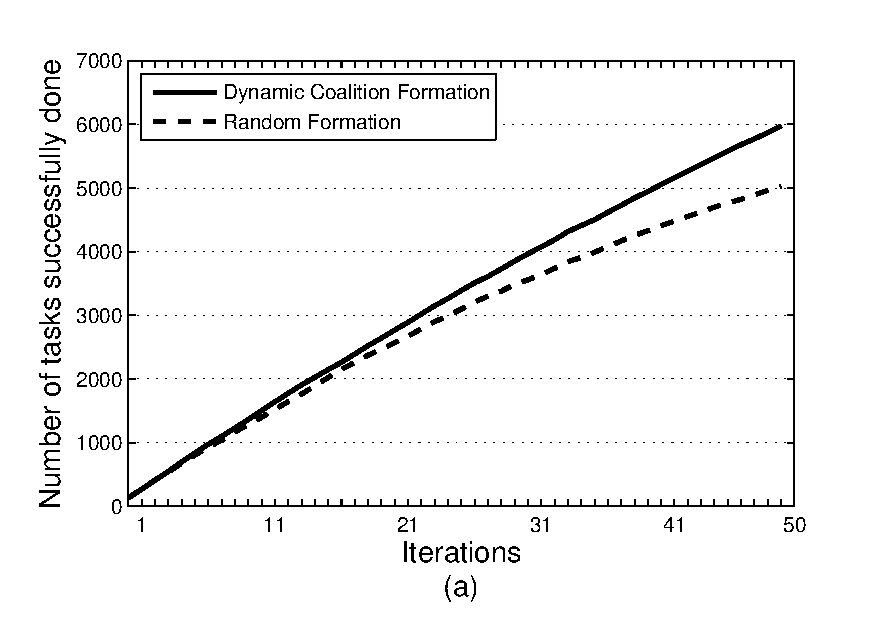
\includegraphics[width=3in]{Figures/s2_task_done.eps}
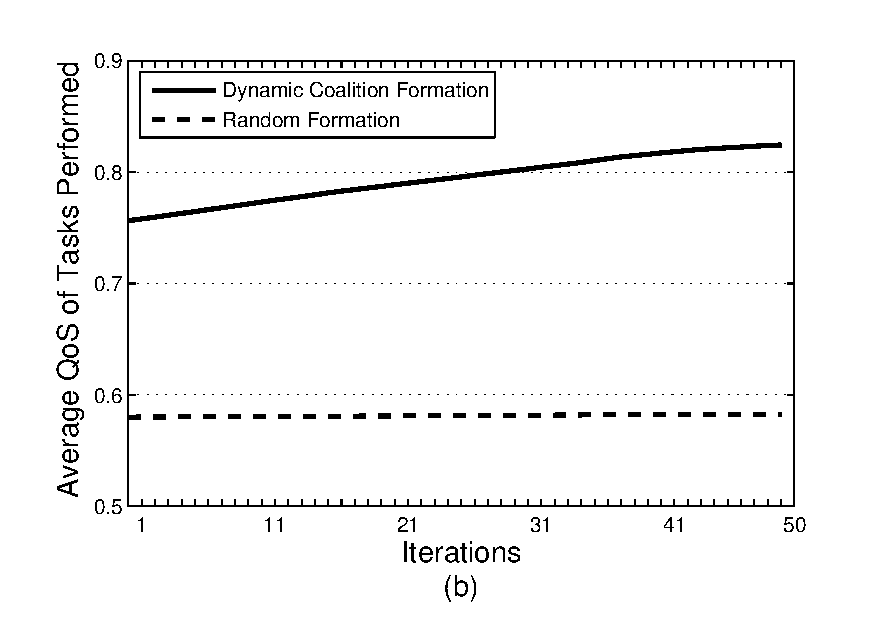
\includegraphics[width=3in]{Figures/s2_task_qos.eps}
\caption{Part (a): Cumulative number of tasks succesfully done. Part
(b): Average QoS of tasks performed.} \label{performancemany}
\end{figure}

In Figure \ref{performancemany}, we compare our \emph{Web Services
and many Communities} scenario with a method which ignores QoS
parameters and forms coalitions by allowing web services to join
only if they have enough requests for themselves. In other words,
web services can join a community when the request rate is less
than the throughput of all the member web services. We name this
method \emph{Random Formation} and use it as a benchmark for our
QoS-aware coalition formation process. In this scenario, each user individually generates randomly
between 0 to 10 number of tasks per iteration, then the users target a community and direct their requests to the chosen community. As the results illustrate,
our method forms better coalitions of web services improving
performance and satisfaction for both web services and coalitions.


\begin{figure*}%[!t]
\centering
%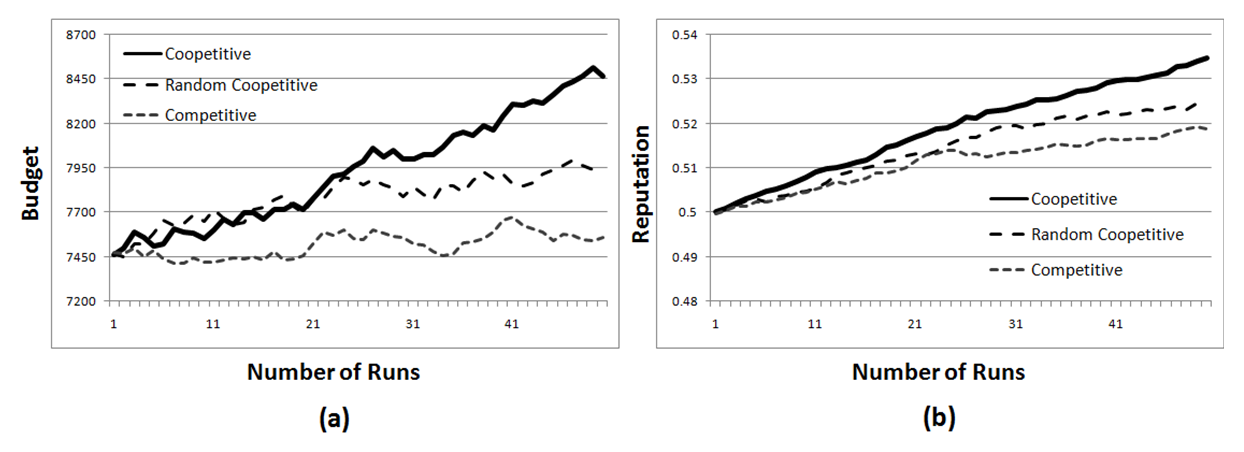
\includegraphics[scale=0.6]{graph1Final+.eps}
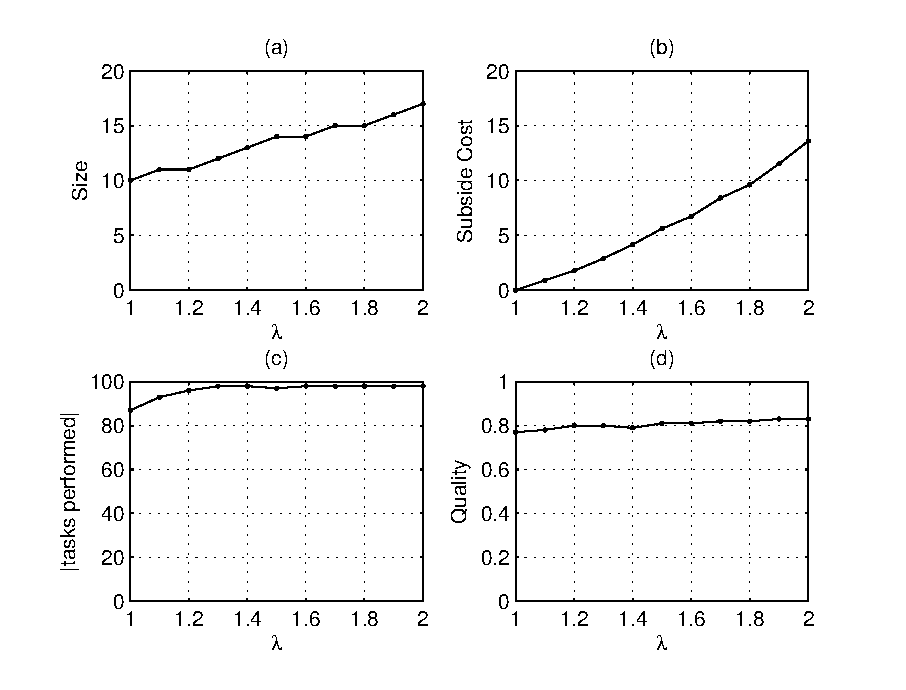
\includegraphics[width=3in]{Figures/taxtation.eps}
\caption{Analysis of community subsiding coefficient $\lambda$ on
average community size (a), cost (b), number of tasks performed
(c), and average quality of service of tasks performed (d).}
\label{f_taxtation}
\end{figure*}

As mentioned in Section \ref{s:tax}, a solution to help the
community stabilize is to subside the community by a relative
coefficient ($\lambda$) so the value of $\lambda v(C)$ is divided
among the community members. We have analyzed the effect of
subsiding and the cost it incurs to our web service communities.
Figure \ref{f_taxtation} shows the results. In this experiment, we
have set a community with input task rate $R_C$ of 100 and having
web services throughput rate $Th_{ws}$ values from a normal
distribution with average 10 tasks per iteration and standard
deviation 2. Part (a) shows the community size increases in a
linear fashion as ($\lambda$) increases. However, the cost (Part
(b)) is having a slight exponential growth rate since, not only
($\lambda$) increases, but also the size of the community is
increasing slowly. Therefore, subsiding can be costly for larger
number of $\lambda$ values. Part (c) depicts the number of tasks
done by the community per iteration. It is obvious that with
$\lambda$ value of 1.3, which is 30\% of the community valuation,
the number of tasks done almost reaches the input task rate cap of
100 tasks per iteration. The average quality of tasks also has a
slight increase since the community will be able to afford better
and more web services to join the community (Part (d)). These
results show the effectiveness of our subsiding method and its
impact on the QoS. In fact, using more than 30\% of the community
valuation as subsidy is not very effective and is costly to
perform.

\begin{figure*}%[!t]In the previous experiment, we considered the scenario where all
web services are stable, will not leave the group, and will
fulfill their promised QoS for a good period of time. However, in
real world scenarios of web services, this is not always the case.
This is the reason why the community coordinator would be interested in paying
web services in order to keep the group reliable from the end
user's point of view.
\centerline{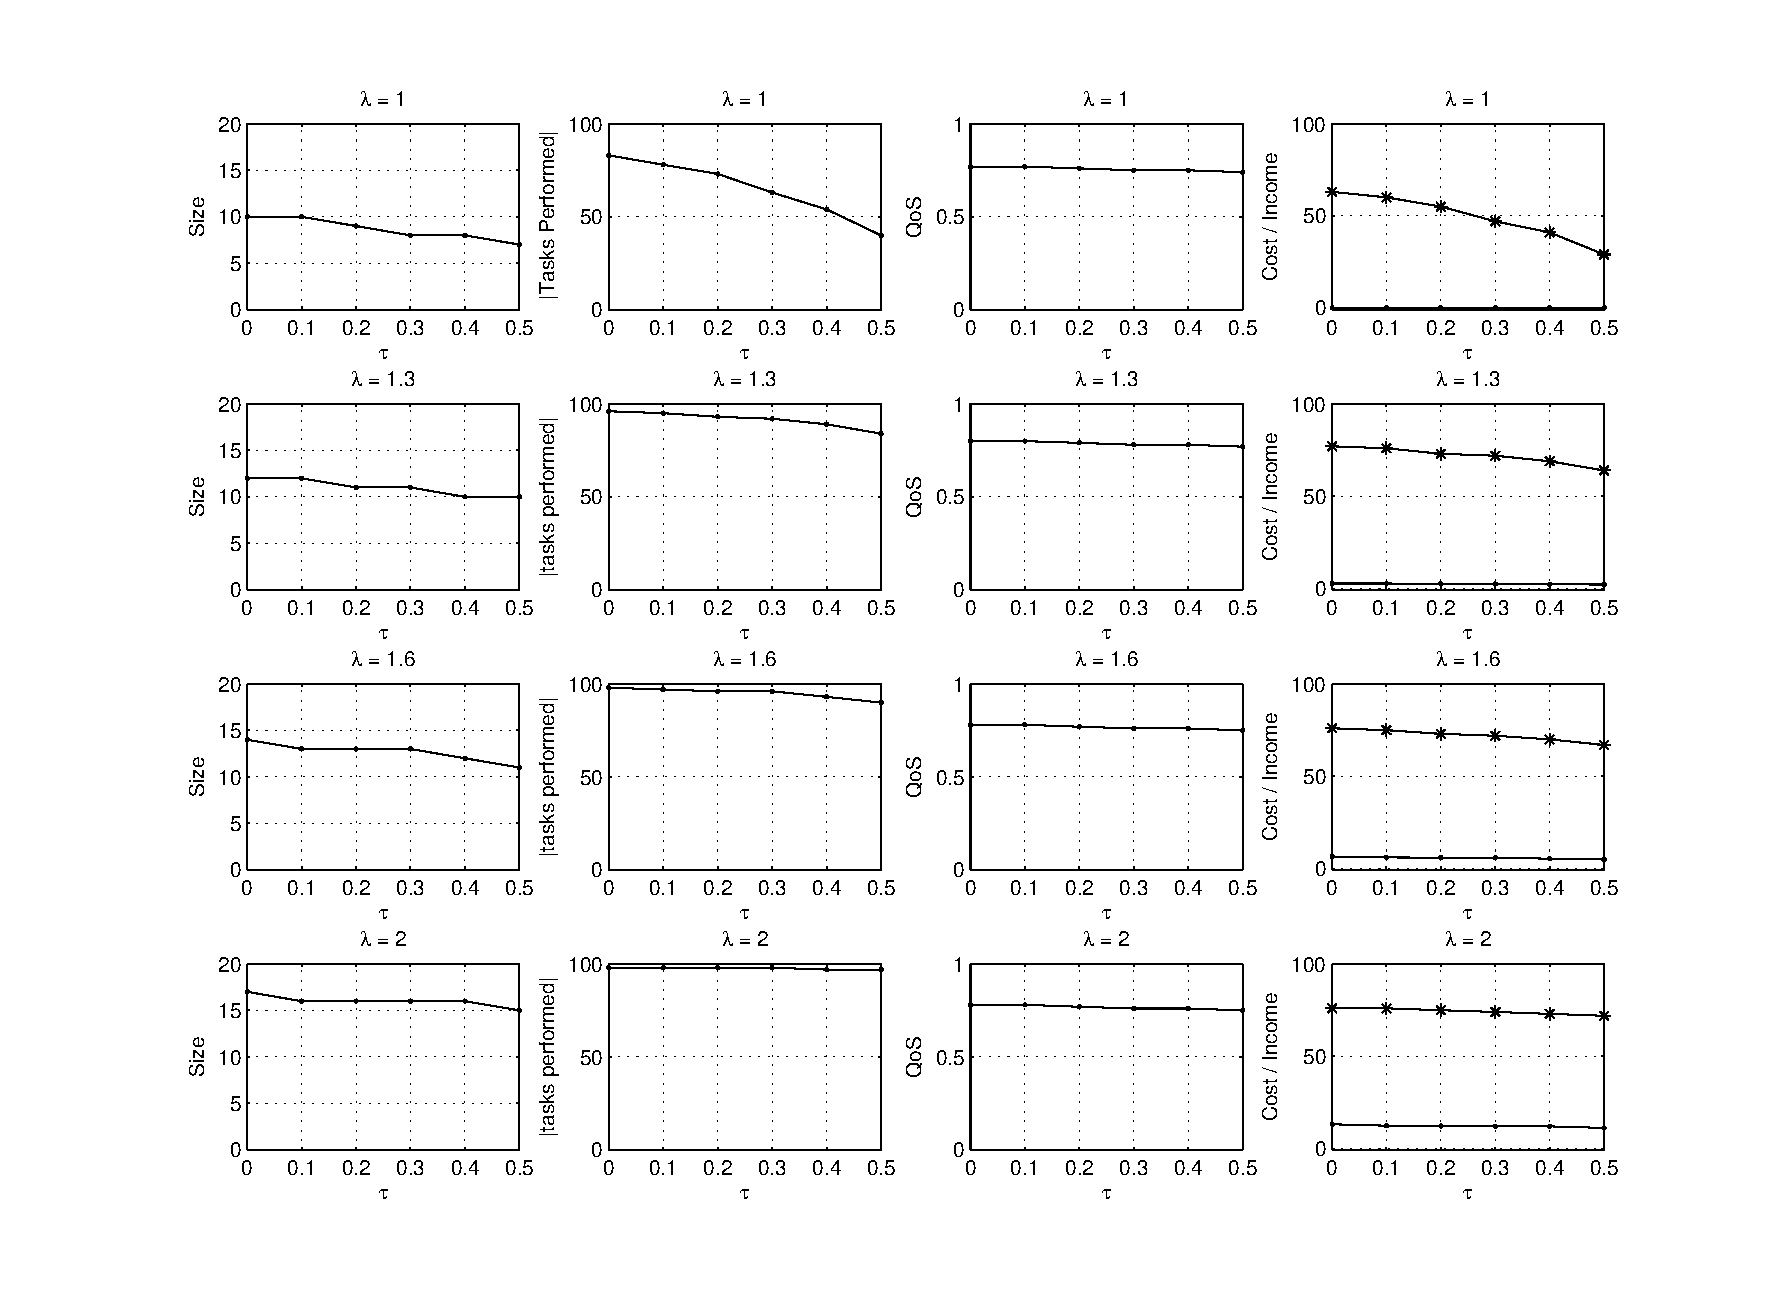
\includegraphics[width=6.8in]{Figures/tax_dyn.eps}}
\caption{Analysis of community subsiding coefficient $\lambda$
having web service different stability levels of $\tau$ on average
community size, number of tasks performed, average quality of
service, and average cost/income of communities.}
\label{fig_dynamic_taxtation}
\end{figure*}


In our next scenario, we have introduced the
new instability variable $\tau$ ranging from 0 to 1, 0 meaning web
services having no instability issues and will perform as they
claimed until the end of the experiment, and 1 meaning very
unstable web services, which will stop functioning on the first
iteration of the community distributing tasks. Figure
\ref{fig_dynamic_taxtation} illustrates the results of our
experiment having web services with average instability values of
0 to 0.5 and having relative subside value $\lambda$ of 1, 1.3,
1.6, and 2. The \emph{Cost/Income} charts on the right column show
that having subside value of 1.3 incurs the least cost and
increases the community income significantly. Subsiding values of
1.6 and 2 yield high cost to the community and only slightly
increase the community revenue. Moreover, the role of subsiding is
much more obvious when we have unstable web services. In scenarios
where web services are 100\% stable, the subsiding cost will
hardly be compensated by the community revenue.

\begin{figure*}%[!t]
\centering
%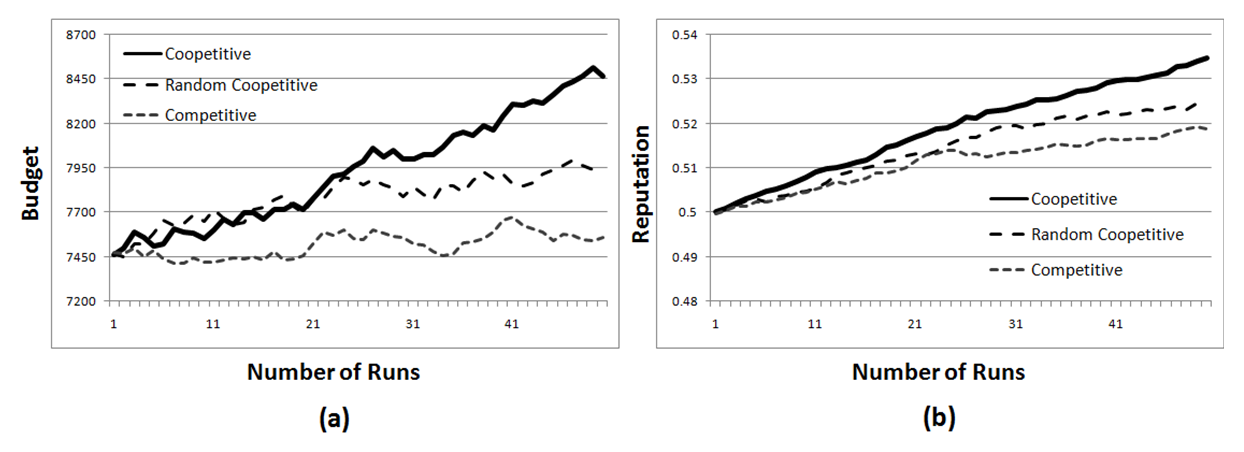
\includegraphics[scale=0.6]{graph1Final+.eps}
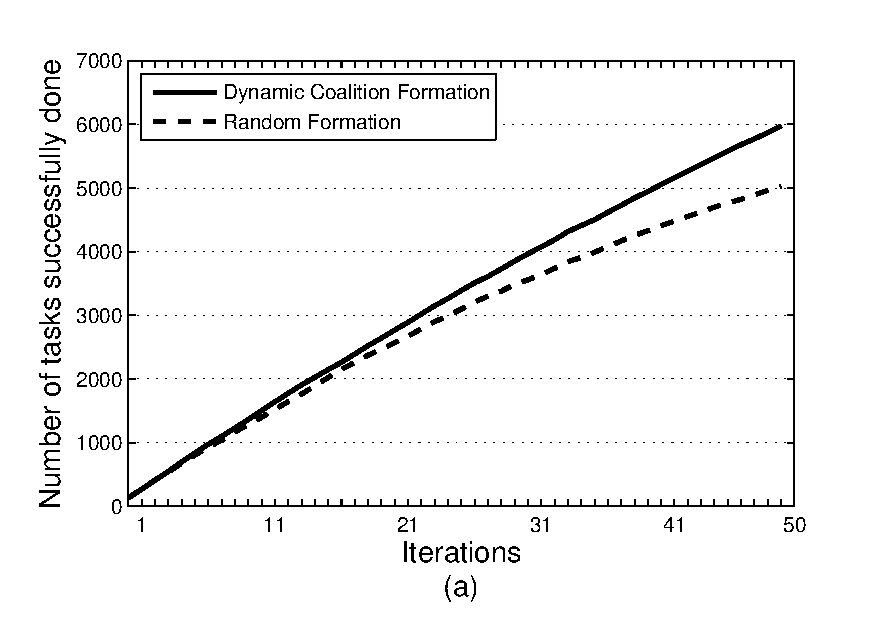
\includegraphics[width=2.5in]{Figures/s2_task_done.eps}
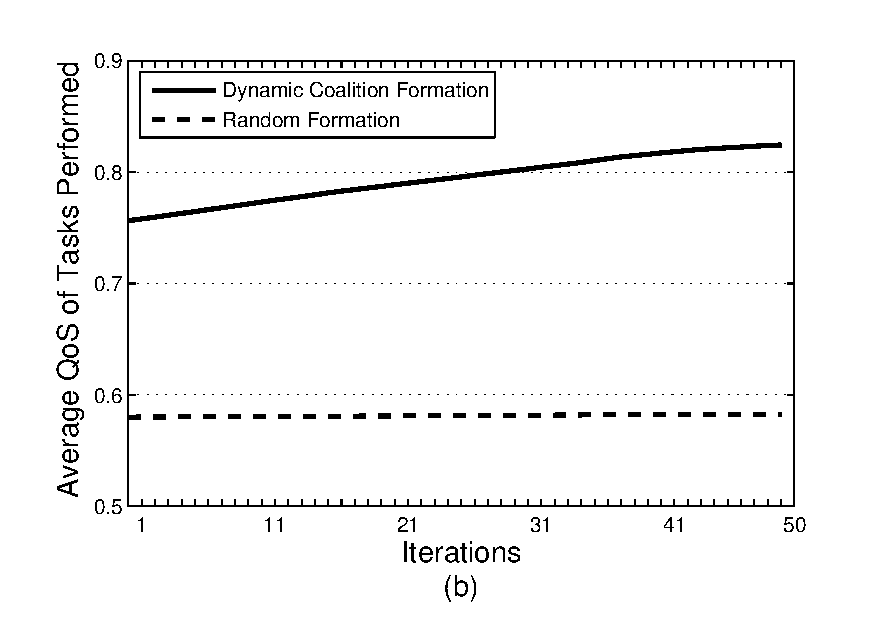
\includegraphics[width=2.5in]{Figures/s2_task_qos.eps}
\caption{Part (a): Cumulative number of tasks successfully done.
Part (b): Average QoS of tasks performed.} \label{performancemany}
\end{figure*}


In Figure \ref{performancemany}, we consider \emph{Web Services
and many Communities} scenario and we compare our dynamic
coalition formation solution with a method which ignores QoS
parameters and forms communities by allowing web services to join
only if they have enough requests for themselves. In other words,
web services can join a community when the request rate is less
than the throughput of all the member web services. We name this
method \emph{Random Formation} and use it as a benchmark for our
QoS-aware community formation process. In this scenario, each user
individually generates randomly between 0 to 10 number of tasks
per iteration, then the users target a community and direct their
requests to the chosen community. As the results illustrate, our
method forms better communities of web services improving
performance and satisfaction for both web services and
communities.

\begin{figure*}%[!t]
\centering
%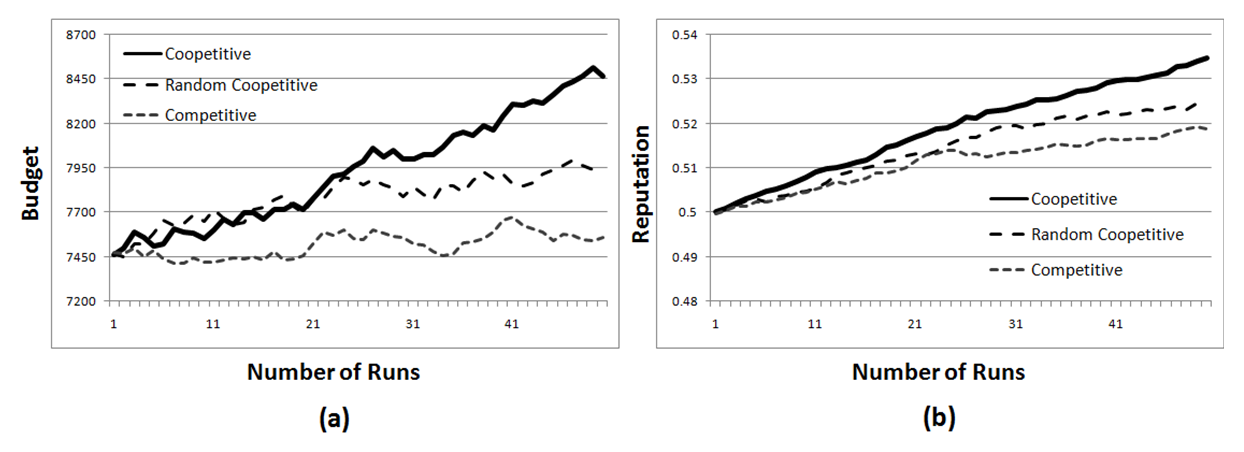
\includegraphics[scale=0.6]{graph1Final+.eps}
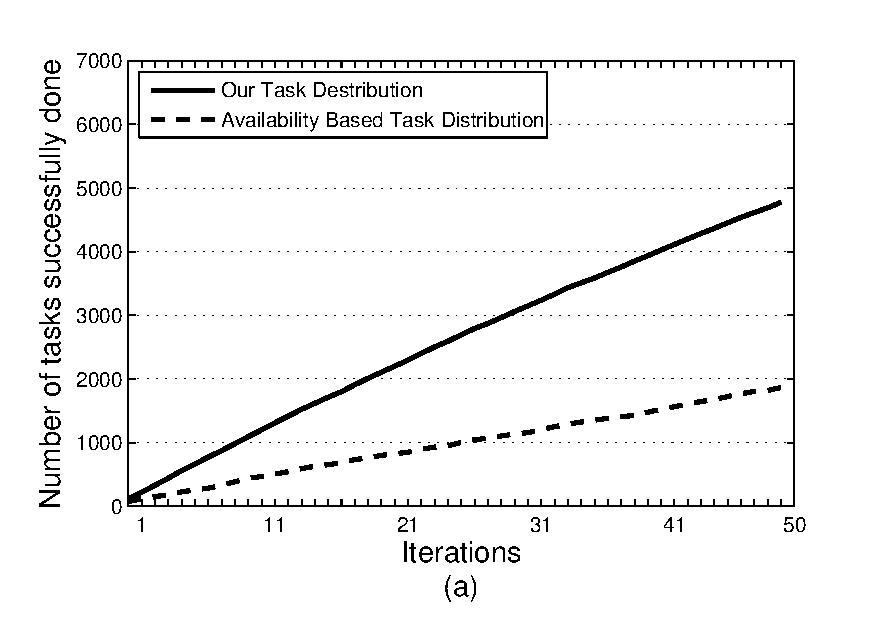
\includegraphics[width=1.9in]{Figures/avg_task_ws_done.eps}
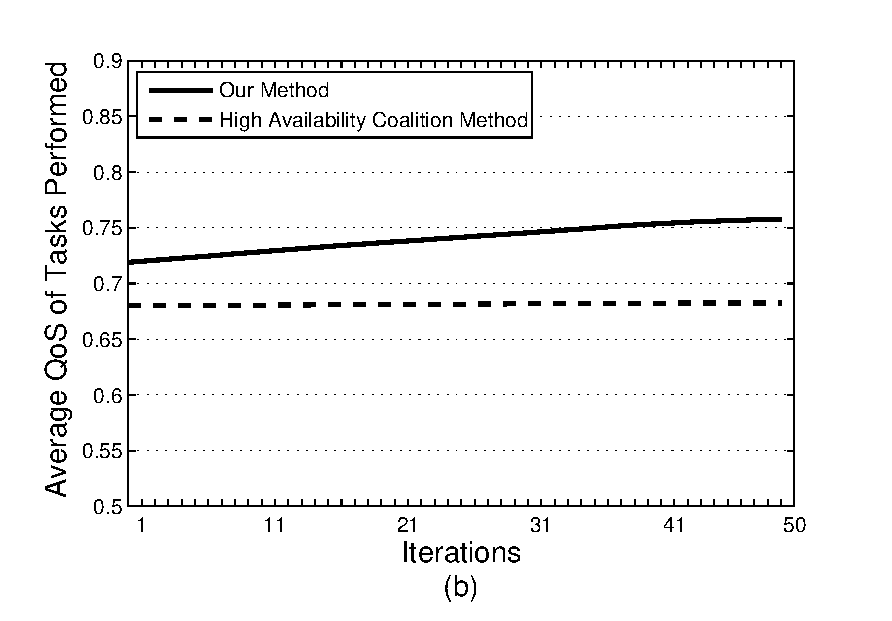
\includegraphics[width=1.9in]{Figures/avg_qos_ws_done.eps}
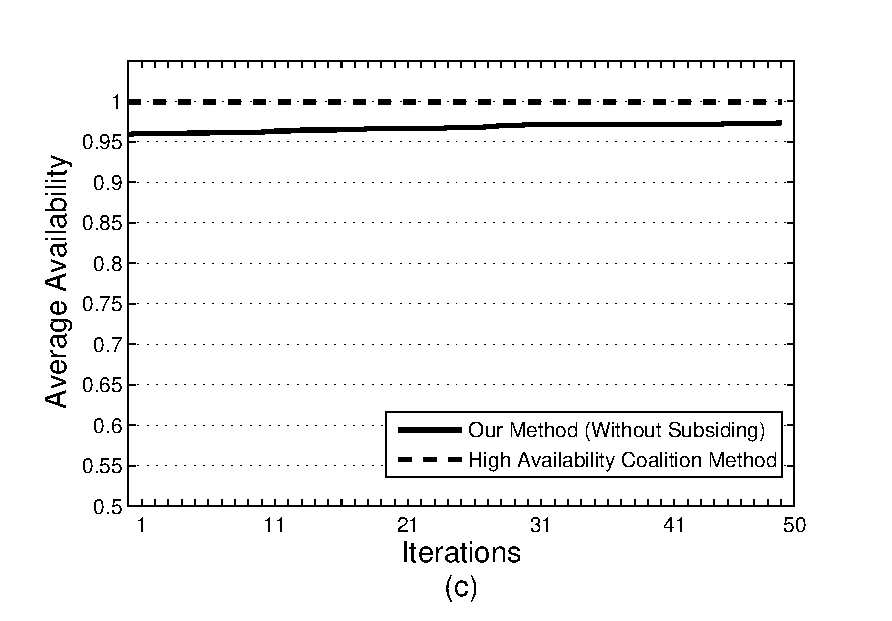
\includegraphics[width=1.9in]{Figures/avg_avail_ws_done.eps}
\caption{A comparison between our community model and the High
Availability Coalition model from \cite{10.1109/TSC.2012.12}. Part
(a): Cumulative number of tasks successfully done. Part (b):
Average QoS of tasks performed. Part (c): Average community
service availability} \label{fig_avail_method}
\end{figure*}

Finally, in our last experiment, we compare our model with the
solution proposed in \cite{10.1109/TSC.2012.12}, which we call
\emph{High Availability Coalition} model. In this method, the
community valuation function focuses on the community availability
as main consideration. The community formation model used in this
method is very different from ours, but we have been very careful
to make the experiment environment as fair and similar to ours as
possible. We limited our maximum community size to 5 in order to
have communities with almost the same size as in
\cite{10.1109/TSC.2012.12}. In the High Availability Coalition
model, the authors have used web services as backups rather than
active collaborative players, and those web services only get a
task when the first web service in an ordered chain fails to
perform that task. %However, with recent advancement in cloud and
%hardware infrastructures, availability is less of an issue for web
%services, and web services are highly available.
Part(a) of Figure \ref{fig_avail_method} shows that with our
method, the number of tasks successfully done is higher with a
rate of three times more than the High Availability Coalition
model thanks to the cooperative behavior of web services and the
task distribution process of our algorithm. This result shows that
using web services as backups, and not as real collaborative
players results in a considerable waste of web services capability
since services have very low chance of getting jobs and its the
primary web service (the first in the coordination chain) which
does most of the work. As shown in Part (b), the average quality
of service of tasks performed using our solution is also higher
since our method considers all quality of service metrics used. Part(c) shows the availability of
communities from the end user's point of view. The High
Availability Coalition model has almost 100\% uptime since web
services are used as backups, so the chance of job failing is
getting reduced significantly as community members increase. In
our method, we have more chance of failure for each web service.
However, with some subsidies and by hiring a few more web
services, the chance of failure of web services in our communities
can be lowered.

\subsection{Coopetitive Behavior}\label{sb:resutlscoop}


%%%%%%%%%%%%%%%%%%%%%%%%%%%%%%%%%%%%%%
\section{Summary}\label{sec:conclusion-cha3}

In this section, we proposed a cooperative game theory-based model for the aggregation of web services within communities. The goal of our services is to maximize efficiency by collaborating and forming stable coalitions. Our method considers stability and fairness for all web services within a community and offers an applicable mechanism for membership requests and selection of web services. The ultimate goal is to increase revenue by improving user satisfaction, which comes from the ability to perform more
tasks with high quality. Simulation results show that our, polynomial in complexity, approximation algorithms provide web services and community owners with applicable and near-optimal
decision making mechanisms. 

As future work in this area, we would like to perform more analytical and theoretical analysis on the convexity condition and also minimal $\epsilon$ values in \emph{$\epsilon$-core} solution concepts based on the characteristic function in web service applications. From web service perspective, the work can be extended to consider web service compositions where a group of web services having different set of skills cooperate to perform composite tasks. Also bargaining theory from cooperating game theory concepts can be used to help web services resolve the instability and unfairness issues by side payments.

In this chapter, we assumed our web services and communities have compelte knowledge of all the other web services and their parameters. In next section we propose distributed decision making model which can perform in scenarios where information is incomplete.


%%%%%%%%%%%%%%%%%%%%%%%%%%%%%%%%%%%%%%%%%%%%%%%%%%%%%%%%%%%%%%%%%%%%%%%%%%%%%%%
%% Chapter 4: On the Interaction between Probabilistic Knowledge and Probabilistic Commitment.
%%%%%%%%%%%%%%%%%%%%%%%%%%%%%%%%%%%%%%%%%%%%%%%%%%%%%%%%%%%%%%%%%%%%%%%%%%%%%%%
\setcounter{chapter}{3}

\chapter{Distributed Decision Making for Dynamic Formation of Web Services Communities}\label{cha:PCTLKC}


\section{Introduction}

Given the dynamic and unpredictable nature of the Internet, delivering high quality services is a critical and challenging issue. One practical solution towards delivering such quality services is utilizing intelligent decision making agents. These agents aim at maximizing their gain by exploring the best ways to provide services that satisfy end users \cite{Zeng:2003:QDW:775152.775211, 10.1109/ARES.2008.7, Demirkan2013412, journals/tsc/ZhengZYB13, Josang:2007:STR:1225318.1225716}. However, agent-based web services are functionally limited in the sense that they cannot handle a large number of requests at the same time without compromising the quality of service provided. Recent developments have attempted to shift web services from simple models, consisting of individual components, to models made up of autonomous and group-based components that share common goals. In group-based models, interaction, composition, and cooperation are the key challenges that directly impact the group's overall performance in achieving common goals \cite{ICWS2011-1, SCC2011-1, journals/mags/BaldoniBM10, journals/jcss/CasadoYT13}. To that end, we see the emergence of web service \emph{communities}, which consist of grouping services with similar functionalities but distinct nonfunctional properties \cite{Zeng:2003:QDW:775152.775211, 10.1109/ARES.2008.7, Paik:2005:TSS:2229263.2230038, Medjahed05adynamic}. A community of web services runs continuous performance assessment functions that regulate web services' interactions and manage their composition and cooperation.

Web Services communities have the advantages of facilitating web service discovery and providing better quality of service compared to individual services. Communities act as abstract web services, communicating with external entities via the same standard protocols that a normal web service employs. The difference is that communities regulate the service process via sophisticated internal communication protocols, thereby providing services based on the combined efforts of a number of web services. The downside to communities is the complexity of management involved in finding and inviting adequate individual services and managing the overall quality of the combined work of several services.
% because although they have similar functionality, they have different attitudes.
When interacting with a community of web services, users send their requests to the coordinator of the community, which plays the role of community representative or access point. The community coordinator is responsible of receiving tasks and delivering services. Moreover, as community representative, it verifies the credentials of new web services before accepting them into the community and kicks services that could harm the value of the community.

\textbf{Challenges and Problem Statement.} In recent work, communities of web services have been proposed in order to facilitate discovery of web services, improve the Quality of Service (QoS), and help individual services find better market share and opportunities \cite{Zeng:2003:QDW:775152.775211, 10.1109/ARES.2008.7, Paik:2005:TSS:2229263.2230038, Medjahed05adynamic}. However,  two important challenges are to be addressed: 1) choice of the best web services during community development from the community perspective; and 2) choice of the best community to join from the web service perspective. The advocated solutions  \cite{10.1109/ARES.2008.7, conf/webist/MaamarLBTS07, journals/soca/XuYLZB11, 10.1109/TSC.2012.12, managing-hela-jalel, DBLP:conf/IEEEscc/KhosravifarABT11, DBLP:conf/IEEEscc/LimTMB12} have attempted to address these challenges. However, those solutions have two main limits:
\begin{enumerate}
	\item The solutions consider the architecture of centralized management for communities where most of the decisions are made by the centralized coordinator. The problem is that in real world scenarios, decisions made by independent service providers are highly distributed.
	\item The solutions either propose complex algorithms \cite{10.1109/TSC.2012.12, DBLP:conf/IEEEscc/LimTMB12, journal-community-formation} to find the optimal strategy to follow, or oversimplify the problem by eliminating important parameters and using approximation techniques to make the algorithms tractable \cite{10.1109/TSC.2012.12}.
\end{enumerate}
These approximation methods sometimes negatively influence the outcome because simplifying the constraints may cause important aspects of the problem to be ignored. For instance, instead of calculating the gain distribution using the adequate, but complex shapely-value method, the authors is \cite{10.1109/TSC.2012.12} propose a simple egalitarian way of distributing gain, which completely ignores the gain generated from collaborative work of sub-communities. Other categories of related work, for instance \cite{10.1109/TSC.2012.12, DBLP:conf/IEEEscc/KhosravifarABT11, DBLP:journals/ijebr/MaamarSTBB09}, restrict the decision process within the community coordinator, so other members of the community are not effectively involved.
%And some other work which do not focus on rationality on web services or communities involved [refrences].
In \cite{journal-community-formation}, we proposed a cooperative game-theory-based model for aggregating web services in communities. A centralized decision maker in communities, based on a complete knowledge of available web service quality metrics and performance, has been used to form optimal and stable communities that maximize individual and group income. However, centrality and complete information are strong assumptions, which are not very compatible with real business scenarios.

\textbf{Contributions.} In this chapter, we introduce DDM, a Distributed Decision Making model for community formation that regulates web service agents’ decision making process in terms of cooperating and deciding which group to join and which service to invite for joining. Unlike existing work on community formation, our decision model is extracted from a data model in the form of information obtained from a large number of web services regarding their single and cooperative utilities as well as environmental parameters such as demand, service quality, etc. The generated decision tree improves agents' understanding of the environment and how to select actions that lead towards maximizing their utilities. The advantage of this approach is that the tree, which is initially created from the past data, reflects a comprehensive vision about agents' attitudes in terms of their action selection based on their past experiences. Moreover, the tree is getting continuously updated based on both new received feedback and the outcome of chosen actions. This continuous update makes the approach adapted to any change in the environment.
%The training model deploys a logistic regression algorithm to build a hypothesis function that can thoroughly address the aforementioned research problems.
The decision model provides web services with enough information which helps those services efficiently decide and predict the outcome of their different possible collaborations. This model works in a distributed manner in which services are self-sufficient in their decision making and do not rely on a centralized decision making process. Our findings show that communities of web services can efficiently find the appropriate web service to invite for cooperation as well as allowing a single web service to find the best communities to join. The proposed model can be seen as a recommneder system that suggests beneficial actions for both communities and single services. Communities can consider the decision model and analyze the characteristics of different individual web services and make prudent decisions when inviting a web service to join or accepting a join inquiry initiated from a web service. In general, DDM equips web services with efficient methods for foreseeing how their choices will impact both their short-term and long-term goals; therefore, opting for the best decision available.

To effectively generate the decision model for web services, we used a real dataset to extract web services' individual characteristics and used them to measure outcomes when these services cooperate with one another. The dataset has been extracted from real-world QoS evaluation results from 142 users on 4,532 Web services during 64 different time slots. Combining the available data based on each web service point of view on different time slots, we acquired 5 different unique features for those 4,532 web services. By engineering and extracting these features, we gathered functional and cooperative features for both individual web services and communities in different time slots. We were able to investigate the path a web service might take to achieve the best utility out of effective interactions with others. All the paths and outcomes are labeled to be utilized in the training model. Using cross validation sets, web services are able to compute the optimal hypothesis function (using logistic regression) that can be used to predict outcomes of cooperative work with other individual web services or communities. Our findings show that web services equipped with DDM have by far better outcomes than the ones that either do not cooperate or randomly find communities to join.

\section{Challenging Issues}\label{s4:preliminaries}
%In this section, we first present the architecture of DDM. We explore the characteristics of intelligent service agents and the features we extract for training. To do this, we first discuss some preliminaries.
In this section, we introduce the challenges behind community formation.

\subsection{The Join Challenge}\label{s:tjc}
It has been showed in \cite{10.1109/ARES.2008.7,10.1109/TSC.2012.12,journal-community-formation} that web services can increase their overall utility by collaborating with other web services within communities. This collaboration provides them with better ways of sharing resources and having higher reputation, greater market share and wider visibility. Web services and communities come with different quality metrics, and the long-term outcome depends on these metrics.

The goal of all parties involved in the community is to maximize their long-term outcome while they are operating as part of the community. Web services need to be equipped with a selection strategy to choose from the different possible collaboration groups they can form as well as an estimation method for evaluating the long-term gain of joining different possible communities. Web services need to experiment with different possible collaborative groups in order to estimate their gain over time. However, with a high number of possible communities, it is not possible to test collaboration with random web services. Even if a linear approximate function for estimating utility based on community web services' parameters is adopted, the exponential \footnote{Bell number: $http://en.wikipedia.org/wiki/Bell\_number$} growth rate of the possible number of partitions of web services into communities would make any brute-force type algorithm for the best community selection strategy intractable and impractical in real-world application settings.

\subsection{Join Consequences}\label{s:jc}
It is worth mentioning that a \emph{join} event takes place as a result of interaction between two parties that are looking to expand their collaborations. All actions are chosen in an attempt to enhance the overall outcome. However, the selected action may result in decreasing the overall utility in the long run.
% long term.
This is the case when a single web service joins a community, but the complex process of task allocation eliminates the visibility of that service, which stays idle within the community. This makes the join action of that service a bad decision. The same event might be beneficial for the community, as it hosts a new web service that can engage in performing a new coming task. But overall, in this particular case, if the new web service stays idle for a long period of time, neither side will benefit from collaborating with the other and the join event will result in negative consequences for at least one side's utility.

The more common scenario is when both parties benefit from the joining of a web service to a community. This joining action is then rational as both the web service and community enhance their utilities. However, the community may not be the best choice for the web service. In other words, the web service could have joined a better community if it had enough and accurate knowledge about the surrounding environment. Since the community does enhance its utility, the web service could stay with that community, which results in a non-optimal increase in web service's utility. In the following section, the proposed model provides solutions that effectively address the aforementioned challenges.

\section{The Model Components}\label{s:themodelcomponents}

In this section, we discuss the parameters that we use in the rest of the chapter. Then, we present the task distribution and revenue model of our distributed web services communities.

\subsection{Internal Features}\label{s:if}

With a group of web services having identical or similar functionalities, QoS metrics provide nonfunctional characteristics for optimal candidate selection. Web services quality metrics have been studied and analyzed in various proposals, for instance in in \cite{Ardagna:2007:ASC:1263152.1263531,Menasce:2002:QIW:613357.613758,10.1109/ISSRE.2011.17}. In this chapter, we adopt the most representative QoS properties of those services that highly influence their utility.
%We refer to a typical web service as ws_{i}.

Let $C = \{ws_1,ws_2,..., ws_n\}$ be a community with $n$ web services. We define the following features for the group of web services based on their functional parameters:

\begin{itemize}

  \item \emph{Throughput} is the rate at which a service can process requests. QoS measures can include the maximum throughput or a function that describes how throughput varies with load intensity. Throughput is a positive real number. For a given community $C$, the expected throughput value $(Th_{C})$ can be estimated as the summation of throughput of all the service members $Th_{w}~ (w \in C)$:
	
	\begin{equation}
		 Th_{C} = \sum_{w \in C}{(Th_{w})}
	\end{equation}
	
	\item \emph{Availability} is the percentage of time that a service is operating. It is computed as
the probability that the service operation is accessible. Availability of a web service $A_w$ is a real number in the range $[0, 1]$. For a community $C$, the expected availability $(A_{C})$ considering the members operate in parallel (independently from each other) can be estimated as:
	
	\begin{equation}
		A_{C} = 1-\prod_{w \in C}{(1-A_{w})}
	\end{equation}
	
	\item \emph{Execution Time} is the time a service takes to respond to various types of requests.
	%is the expected delay between the time instant when a request is sent and the time when the result is obtained.
	Execution time is usually measured in milliseconds and can be affected by load intensity, which can be measured in terms of arrival rates (such as requests per second) or number of concurrent requests. This internal feature is a positive integer. For a typical community $C$, the expected execution time $Et_{C}$ can be estimated as the execution time of the bottleneck service which is the service with the slowest execution time $Et_{w}$:
	
	\begin{equation}
		Et_{C} = max_{w \in C}{(Et_{w})}
	\end{equation}
	
	%\item \emph{Data Quality} The ability of a data collection to meet user requirements , defined as the proximity of a value v returned by web service to a value considered as correct. The measure of data quality is considered here as a real number in the range [0, 1], where 1 represents the most desirable score.
\end{itemize}


	We normalize the range of these features so that each feature contributes proportionally to the final utility outcome value. We adopt the \emph{standardization} method consisting of subtracting the \emph{mean} from each feature, then dividing the subtraction result by the \emph{standard deviation}.

%$HI = \overline{HI}$

\subsection{External Features}\label{s:ef}

The quantitative values of quality metrics need some benchmark values to represent their goodness. In fact, without some benchmark values, it would be difficult for web services to identify their performance quality at any specific value of these metrics. Therefore, we introduce two external features for assessing web services' estimate with regard to their standing among other web services.

\begin{itemize}
  \item \emph{External Parameter 1} ($Exp1_i$ where $i$ is a community or a web service) is an estimate of how close the community's or the web service's \emph{execution time} is to the best execution time in the whole system. It is the difference between a community's or a web service's \emph{execution time} metric and the minimum value of execution time of all the other communities or web services. The smaller the value the better the external feature compared to other peers. In other words, small value of $Exp1_i$ means $i$ is among the best communities or services in the system.
	\begin{equation}\label{exp_1:f}
		Exp1_i = Et_{i} - Et_{min}
	\end{equation}
	\item \emph{External Parameter 2} ($Exp2_i$ where $i$ is a community or a web service)  is a comparison of the community's or the web service's rate of performing tasks to the best rate in the system. It is the difference between a community's or a web service's \emph{throughput} metric and the maximum value of throughput in the system. As for $Exp1_i$, the smaller the value the better the external feature.
	\begin{equation}\label{exp_2Lf}
		Exp2_i = Th_{max} - Th_{i}
	\end{equation}
\end{itemize}

\subsection{Task Distribution}

Communities of web services usually employ an implementation of Contract-Net protocol for task distribution, in which services bid on incoming tasks, and receive some of the tasks for which they bid \cite{DBLP:journals/ijebr/MaamarSTBB09,DBLP:conf/aina/ElnaffarMYBT08}. In our model, our community members would try to distribute tasks based on their capabilities and the QoS parameters provided by the web services. We use a slightly modified \emph{weighted fair queuing} method to distribute tasks among community members. The goal is to allocate incoming tasks to web services with a rate matching the throughput value of $Th_{w}$ for each web service $w$. In the \emph{weighted fair queuing} method, the input flow is multiplexed along different paths. However, in our model, if the rate of incoming tasks is less than the community's total throughput $(Th_{C})$, which is the summation of throughput values of the web services in the community, some of the input tasks will be queued and served with a delay.
%Thus, the amount of tasks performed by the community is $\sum_{ws}{Th_{ws}}$ when $\sum_{ws}{Th_{ws}} \leq R_{C}$.
When the incoming task rate is less than the throughput of the community, the \emph{weighted fair queuing} algorithm assigns a weighted task rate of $Itr \times \frac{Th_{w}}{\sum_{w}{Th_{w}}}$ for each web service $w$ within the community, where $Itr$ is the input task rate.

While distributing tasks, the community can verify the performance, throughput and quality of service of tasks being performed by web services. The community can assess if those web services are capable of performing the number of tasks they advertised. If for any reason, there is a decline in the quality metric or throughput, the community can consider the new values as a benchmark for future performance calculations, and penalize the suspicious web services. This way, players will have incentive to truthfully disclose their actual capabilities in order to maximize profit from the community and to avoid being penalized. In addition, the system should be dynamic enough to detect and react to web services' quality metrics variation, as over time, web service metrics may degrade or improve, changes to which the community should adjust.
% Therefore its easy for the system to encourage players to be in some sense incentive compatible in the way that they would profit best by truthfully revealing their capabilities. Also it is important to be dynamic enough to consider web services which may have their quality metrics degraded or even improved over time for any reason and be able to adjust the community with new parameters.

\subsection{Community Revenue}

Communities and web services earn revenue by performing tasks. The total gain is a function of the quality and rate of performing tasks. The utility of a collaborative group of services $U_{C}$ (i.e., the revenue of the community) is a function of internal and external parameters:

\begin{equation}\label{u_c_general}
U_{C} = f(A_{C}, Et_{C}, Exp1_{C}, Exp2_{C}, Th_{C})
\end{equation}
%
where $f$ is increasing in $A_{C}$ and $Th_{C}$ and decreasing in $Et_{C}, Exp1_{C}$ and $Exp2_{C}$. An example of this function is given in Equation \ref{u_c_normal}:

\begin{equation}\label{u_c_normal}
U_{C} = \big((\alpha \times (A_{C} - Et_{C}) - \beta \times (exp1_{C} + exp2_{C})\big) \times Th_{C}
\end{equation}

The $\alpha$ and $\beta$ parameters are internal and external weight coefficients. Small values for execution time and external parameters ensure better performance, which justifies their negative coefficients. The result is then multiplied by the throughput value $Th_{C}$, since communities are performing tasks with $Th_{C}$ rate.

\begin{theorem}
The function given in Equation \ref{u_c_normal} satisfies the properties of $f$.
\end{theorem}

The proof of this theorem is straightforward by simply calculating the partial derivative $\partial f$ with respect to the different variables.


The estimation of the utility can be improved, especially in cases where the input task rate is high and services are experiencing high task loads. The \emph{weighted fair queuing} method of task distribution would distribute tasks based on the individual throughput $(Th_{w})$ value of services within community. In fact, services having higher throughput affect strongly the overall utility of the community because they would take on proportionality more tasks. The improved utility is given as a function of individual internal and external parameters:


\begin{equation}\label{improved_u_c_general}
U_{C} = g_{w\in C}(A_{w}, Et_{w}, Exp1_{w}, Exp2_{w}, Th_{w})
\end{equation}
%
where $g_{w\in C}$ is increasing in $A_{w}$ and $Th_{w}$ and decreasing in $Et_{w}, Exp1_{w}$ and $Exp2_{w}$. An example of this function is given in Equation \ref{u_c_load}:


\begin{equation}\label{u_c_load}
\begin{split}
U_{C} = \sum_{w \in C}&\bigg(\big(\alpha \times (A_{w} - Et_{w}) \\
        & - \beta \times (Exp1_{w} + Exp2_{w})\big) \times Th_{w}\bigg)
\end{split}
\end{equation}

The following theorem holds:

\begin{theorem}
The function given in Equation \ref{u_c_load} satisfies the properties of $g_{w\in C}$.
\end{theorem}


\section{The Decision Making Mechanism}\label{s:model}

In this section, we describe our data extraction process and the methodology used to equip web services and communities with a decision making mechanism. In this methodology, we first present the data extraction and engineering process and then we evaluate the decision making mechanism for web services in community settings. Figure \ref{fig_steps} summarizes the steps performed in DDM from the input data to the generation of decision making profiles for web services and communities. The objective is to use the input data to build a decision tree for each service and community included in the data set, which will be be served as a benchmark for other services and communities in their decision making mechanism. The decision tree is made up by training the real data obtained from operating web services and extracting features related to their performance, either alone or as part of a joint effort with other web services. The ultimate objective is to propose for each web service and community the best joint decision about forming a group that maximizes every one's utility. The DDM's steps are explained in the following sections.

\begin{figure}%[!t]
\centerline{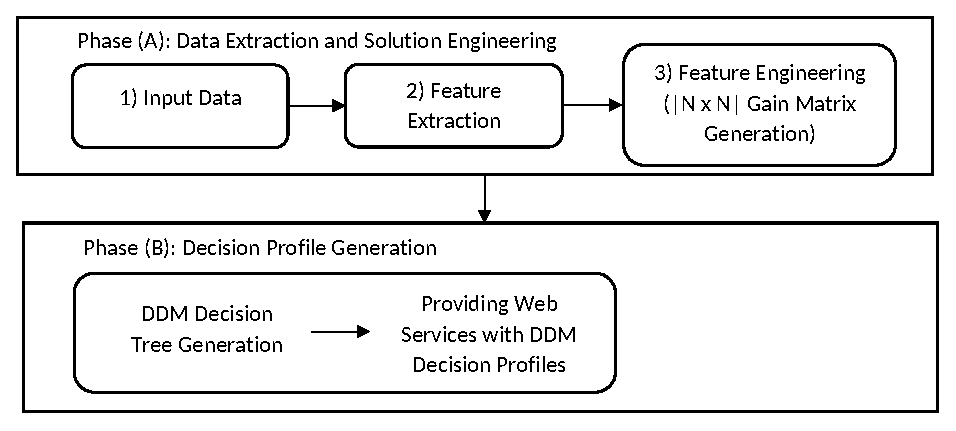
\includegraphics[width=5.25in]{figures/steps.eps}}
\caption{A summary of DDM decision profile generation steps}
\label{fig_steps}
\end{figure}

\subsection{Data Extraction and Solution Engineering}\label{ss:learningdata}

\subsubsection{Input Web Services Data}\label{sss:webservices}

%We used a data set extracted from running web services. In this data set,
Each web service is associated with a number of quality metrics that reflect its non functional parameters. These web services operate in an online environment and are continuously assigned tasks to handle. %To engage in communities, we add the external features that reflect web services' utility as a result of joining other web services to form a community (see Section \ref{s:ef}). %The additional features are %computed based on two assumptions that we adopt for a community to be formed.
We used the web services data set provided in \cite{10.1109/ISSRE.2011.17}. The raw data provides real-world QoS evaluation results from several users on 5,825 web services over 64 different time frames\footnote{http://www.wsdream.net/}. %In this data set, each web service is associated with a number of features that reflect its functionality.
%Our raw data set provides us with 64 different time slots of extracted features for each web service.
Using this data, we built a synthetic data set that contains features of a large number of web services and communities in different time intervals. The goal is to use the data set to train a decision-making model that adopts the trend of joining a community and use the model to predict/find the appropriate community for other web services. %To train our model, we build a decision tree as a benchmark for our decision making mechanism. The decision tree is made up by training the real data obtained from operating web services and extracting features related to their performance, either alone or as part of a joint effort with other web services. The ultimate objective is to propose for each web service and community the best joint decision about forming a group that maximizes every one's utility.

\subsubsection{Feature Extraction}\label{sss:filtereddata}

By processing the data provided for each web service over different time slots, we obtain the three internal quality features introduced in Section \ref{s:if}: \emph{throughput}, \emph{availability} and \emph{execution time} and the two external features discussed in Section \ref{s:ef}.  In fact, web services and communities are represented using feature vectors of these five internal and external features.

%To engage in communities, we add two additional external features that reflect web services estimation of its quality metrics compared to other web services.
%Therefore, we have generated an array of web services with three distinct features.

\begin{figure}%[!t]
\centerline{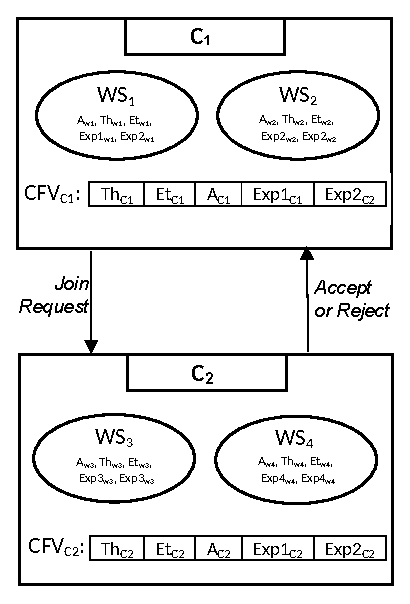
\includegraphics[width=3.15in]{figures/cfvs.eps}}
\caption{Communities with different properties of web services actively looking for other communities to collaborate with}
\label{fig_community}
\end{figure}

%By combining these three internal features to the two external features discussed in Section \ref{s:ef} that reflect the community's estimation of its quality metrics, we generate a set of feature vectors representing the communities of web services for training purposes.


We formulate a \emph{Community Feature Vector (CFV)} as $CFV_{<C>} = [f_1,...f_5]$ having a community of $k$ web services ($C = \{ws_1,...ws_k\}$, $k \geq 1$)\footnote{A web service is considered as a community of one web service.}. The features $f_1$ through $f_5$ represent the \emph{execution time}, \emph{throughput}, \emph{availability} and the \emph{external parameters 1 and 2} respectively. A set of communities, with their feature vectors and utilities evaluated, provides our algorithm with a raw training data set. We call this set of communities the \emph{template vector} $CS$, and the set of feature vectors associated with the \emph{template vector} is referred to as the \emph{community feature vector set (CFVS)}. Figure \ref{fig_community} depicts web services and communities looking to form new groups in order to improve their utility gain.

\subsubsection{Feature Engineering}\label{sss:feng}
Let $CFVS = \{CFV_{<C_1>}, \dots, CFV_{<C_N>}\}$ be the community feature vector set with $N$ communities. Based on the $CFVS$ set, we create an $|N \times N|$ gain matrix $gain^{t}$ for each time slot $t$. Each entry $gain_{n,m}^{t}$ corresponds to a utility gain of community $C_n$ when it joins community $C_m$. This gain is computed as follows: $gain_{n,m}^{t} = U_{C_n \cup C_m}^{t} - U_{C_{n}}^{t}$ where $U_{C_n \cup C_m}^{t}$ and $U_{C_{n}}^{t}$ are the utilities at time $t$ computed using Equation \ref{u_c_load}.  Evaluating the utility gain for all entries of the $gain^t$ matrix is a computationally heavy process when $N$, the size  of the feature vector set, is large. Therefore, this size should be chosen carefully.

\begin{table*}[ht]
\footnotesize
\caption{An example of $gain$ matrix for 3 different communities and their combinations} % title of Table
\centering % used for centering table
{\renewcommand{\arraystretch}{1.2}
\begin{tabular}{c|c c c c c c} % centered columns (4 columns)
\hline\hline %inserts double horizontal lines
 & \textless348\textgreater & \textless1934\textgreater & \textless2117\textgreater & \textless348, 1934\textgreater & \textless1934, 2117\textgreater & \textless348, 1934, 2117\textgreater \\ [0.5ex] % inserts table
%heading
\hline % inserts single horizontal line
\textless348\textgreater & - & 0.282708 & 1.027081 & 0.282708 & 18.027081 & 18.027081 \\
\textless1934\textgreater & -2.637483 & - & 6.969072 & -2.637483 & 5.509583 & 4.387725 \\
\textless2117\textgreater & 5.027081 & 2.969072 & - & 5.509583 & 2.969072 & 5.509583 \\
\textless348, 1934\textgreater & 0.0 & 0.0 & -3.851432 & - & -3.851432 & -3.851432 \\
\textless1934, 2117\textgreater & 2.969072 & 0.0 & 0.0 & 2.969072 & - & 2.969072 \\
\textless348, 1934, 2117\textgreater & 0.0 & 0.0 & 0.0 & 0.0 & 0.0 & - \\ [1ex] % [1ex] adds vertical space
\hline %inserts single line
\end{tabular}
}
\label{table:nonlin} % is used to refer this table in the text
\end{table*}

%Now, we let our set of communities in the $CFVS$ set, within $|T|$ time frame iterations, choose the the best communities to join.
Each community is provided with the corresponding row of data from the $gain^t$ matrix. Basically, $C_i$ is provided with the data in row $i$ of this matrix, which reports all the possible utility values $C_i$ can gain by joining different communities. By ordering the utility gain values of the row, each community is equipped with an ordered set of preferences over other communities it can join. We define $\geq_{i}^t$ as the preference order of community $i$ at time $t$.

Let $C_1 \geq_{i}^t C_2 \geq_{i}^t ~\dots~ C_{i-1} \geq_{i}^t C_{i+1} \geq_{i}^t ~\dots~ C_n$ be an ordered sequence of preferences for community $C_i$ at time $t$. Based on this sequence, we define $K^t(C_i, k)$ as a set of the $k$ most preferred communities of community $i$ at time $t$.
%\subsubsection{feature vector generation}\label{sss:fvg}
\begin{equation}\label{h_t_pref_top}
\begin{split}				
K^t(C_i, 0) = &\emptyset \\
K^t(C_i, k) = &\Big\{C_x | C_x \geq_{i}^t C_y ~\forall C_y \in CS ~\wedge~ C_x \neq C_y ~\wedge~ C_y \notin K^t(C_i, k-1) \Big\}				
\end{split}
\end{equation}
Based on $K^t(C_i, k)$, we define a set of communities $C_j$ for $C_i$ which are the $k$ most preferred communities for $C_i$ and $C_i$ belongs to the $k$ most preferred communities of $C_j$. This basically yields the preference in both sides.
\begin{equation}\label{l_t_top_both}
\begin{split}	
L^t(C_i,k) = \Big\{C_j | C_j \in K^t(C_i, k)~ \wedge~ C_i \in K^t(C_j, k)\Big\}
\end{split}
\end{equation}

Table \ref{table:nonlin} illustrates an example of a $gain$ matrix for 3 different communities and their combinations. Each row shows the gain the community can achieve by collaborating with other 5 communities. In this example, for community $\textless 348 \textgreater$ we have: \\
$K(\textless 348 \textgreater, 1) = \{\textless1934, 2117\textgreater\}$ and \\
$K(\textless 348 \textgreater, 2) = \{\textless1934, 2117\textgreater, \textless1934\textgreater\}$ \\
Since $\textless 348 \textgreater$ is the best preferred community of $\textless 1934, 2117 \textgreater$ and vice versa, therefore $L(\textless 348 \textgreater, 1)$ is not empty and contains the community $\textless1934, 2117\textgreater$.

Using the $gain$ matrix and the mentioned preference ordering relations, we are able to build a decision tree where the list of possible communities to join and their expected utilities are set.
% as well as the joined events that took place in different time slots.
In addition to the best choice, web services have access to other ordered choices and can look for the second best or third best if their first try is rejected by the target community. This aspect is analyzed in more detail in the following section, in which we launch experiments and investigate the effectiveness of the use of a decision tree with different decision layers in joining other communities and enhancing the overall utility.

\subsection{Decision Profile Generation}\label{ss:learningmodel}

Our goal is to create a decision making profile for each community in the
$CFVS$ set. We are creating an environment where the communities can experience the
outcomes of different strategies. The result will be a decision tree of the
feasible and utility-increasing moves over time. The root of the decision tree
represents a community in the $CFVS$ set, and the other nodes represent
the communities resulting from the parent node's action of joining them along with their feature values and
expected utility.


We let communities pick the best communities maximizing their utilities over different time frames. At time $t = 1$, we let each community in the $CFVS$ set choose the best community, which is a single community in the set $\{C_j\} = K^t(C_i, 1)$. If community $C_j$ also ranks $C_i$ to be the highest preferred community to join, meaning the set $L^t(C_i, k=1)$ is not empty, they would join each other. Having set $k = 1$ is a very strict and hardly satisfiable condition. In order to relax the requirement, we increase the value of $k$ by a rate $r$ proportional to time slot $t$: $k = 1 + |r \times t|$. On early steps of the training process, web services and communities are more strict, but as time goes on, we let them choose second and then third best options too. However, increasing $k$  increases the time complexity as well.

When communities $C_i$ and $C_j$ are in each other's top $k$ preference set, the new combined community, i.e., $C_i \cup C_j$ is added to the list of possible communities that can join others at time $t+1$. Moreover, for each community $C_i$ in our initial $CFVS$ set, we maintain a tree with the community $C_i$ as its root. Its children are all the communities that $C_i$ decided to join. As the scenario progresses over time, the merged communities may decide to join other communities. When communities $C_i$ and $C_j$ decide to join each other and create community $C_k$, the new community $C_k$ will be added as a child to both $C_i$ and $C_j$ nodes. At the end of the process, each community is utilized with a tree representing all possible combinations of communities it can join. Algorithm \ref{algo:dectree} illustrates the DDM tree creation procedure as pseudo-code.

\begin{algorithm}
\DontPrintSemicolon
\KwIn{$\langle r, gain^t_{n,n}, CFVS \rangle$ learning rate $r$, $|N \times N \times T|$ gain matrix, community feature vector}
\KwOut{A set of \emph{root} nodes of the decision trees}
$k \gets 1$\;
$nodes[N] \gets$ initialize $N$ tree nodes representing each community in CFVS\;
\For{$t \gets 1$ \textbf{to} $T$} {
	$k \gets 1 + round (r \times t)$\;
  \For{all $C_i \in CFVS$} {
	  \For{all $C_j \in L^t(C_i, k)$} {
      % The "l" before the If makes it so it does not expand to a second line
      \If{$C_i \in L^t(C_j, k)$}{
        $C_k \gets C_i \cup C_j$\;
				add $C_k$ to $CFVS$ set\;
				initiate $node_k$, representing $C_k$\;
				$nodes_i.addChild (node_k)$\;
				$nodes_j.addChild (node_k)$\;
      }
%      \Else{
%        $j \gets j + 1$\;
%      }			
		}
  }
%  $i \gets i + 1$\;
}
\Return{nodes}\;
\caption{{\sc DDM Decision Tree Algorithm}}
\label{algo:dectree}
\end{algorithm}

Having created $|n|$ trees, one per community, our communities are utilized with the different possible paths they can take to maximize their utilities. Using a distance function\footnote{See Section \ref{s:experiments} for an example of this function.}, communities and web services outside the training set can find the community that closely resembles their parameters within the $CFVS$ set. Those new communities can use the trees of the closest communities in the training set to have an estimation of the outcome of all possible joining actions they can take. By so doing, new communities can request to join the best communities which will maximize their gain. Such a request is most likely to be accepted as the decision considers the preferences and utility gain of the other side as well.

As a real scenario example from the used data set, Figure \ref{fig_tree} depicts a snapshot from a decision tree created by the DDM algorithm for a particular singleton community $C_{1273}$. This tree shows the different communities that $C_{1273}$ has experienced with during the training process. Each line shows the web services list within a community, the community's feature vector and the last value on each line is the overall gained  utility of the community.


\begin{figure}%[!t]
\centerline{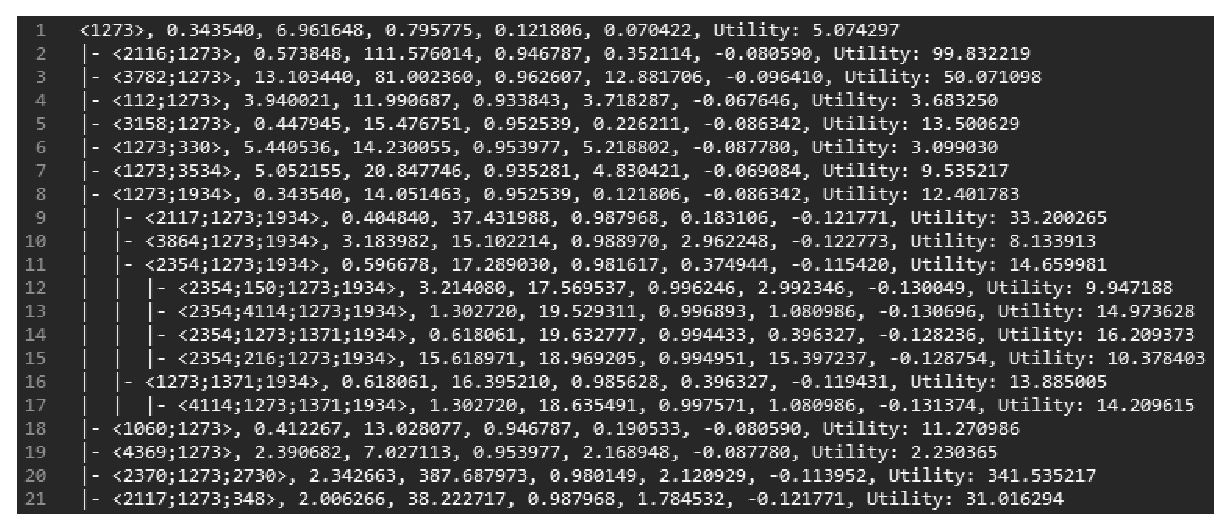
\includegraphics[width=6.25in]{figures/tree1.eps}}
\caption{A partial view of a decision tree created by DDM}
\label{fig_tree}
\end{figure}

\textbf{Complexity.} Here we analyze the computational complexity of the DDM decision tree creation algorithm on each time iteration $t$. Computing top $k$ preferred communities for $C_i$ in $K^t(C_i, k)$ requires $O(n.log(n))$ sort time. The size of $K^t(C_i, k)$ is $k$, and for each of those $k$ communities, we need to check against their $k$ top preferred communities, which needs $O(k^2)$. Line 5 iterates through $n$ communities, Line 6 takes $O(n.log(n))$ to compute and iterates $k$ times, and considering we already have the list sorted, Line 7 can reuse the sorted preferences. Thus, Line 7 takes $O(k)$ time to check if $C_i$ is member of $K^t(C_i, k)$. Multiplying these iterations, the order of complexity of the algorithm with regard to $n$ and $k$ for each time slot is: $O(k^2 \times n^2.log(n))$. Since the whole algorithm runs $T$ times, the overall complexity is $O(T \times k^2 \times n^2.log(n))$.

\section{Experiments}\label{s:experiments}
We implemented DDM in Java\footnote{Source code of implementation and data is available at: $https://github.com/Marooned202/DDM$}. We recall that we have extracted the set of features for 4532 web services in 64 different time slots through a data set provided in \cite{10.1109/ISSRE.2011.17}. By randomly choosing 86 web services out of this data set for each run, and selecting a subset of all possible combinations of sizes 2, 3, and 4 of these 86 web services, we have been able to create 10,000 communities and evaluated the feature vectors and utilities they can have in the 64 time slots. This provides us with the initial training feature set of size $|CFVS| = 10,000$ communities. Based on Equation \ref{u_c_load}, the utilities of these communities are estimated, and then the $gain$ matrix of size $|10,000 \times~ 10,000|$ of all possible ways of merging these 10,000 communities is generated\footnote {The template vector and $gain$ matrix generated are available at $https://github.com/Marooned202/DDM/tree/master/wsds/data/run$}. Based on the $gain$ matrix, each community has an ordered preference among other communities in the set.

We let communities and web services adopt their strategies based on our $DDM$ decision making mechanism. Based on the decisions adopted, each community will generate a decision tree profile. We let DDM run four times with different $r$ rates of 0.05, 0.07, 0.10 and 0.20. With the slow rate of $r = 0.05$, we increase $k$ in Equation \ref{u_c_normal} for every 20 time frames, which will happen only three times in our 64-step experiment. In the case of $r = 0.20$, $k$ increases much faster, at a rate of once every 5 time frames, which increases the complexity of the $L^t(C_i,k)$ search for each community in the $CFVS$ set.

Table \ref{table:valueandgain} depicts the average utility gain value of the communities in each of the four runs. The utility gain is the increase of utility the communities gain by cooperating and joining other communities. The utility gain ratio is the ratio of their final utility over initial utility. Comparing the different search rates, we can see that increasing the value of $r$ from $0.05$ to $0.10$ results in a significant performance boost. However, higher rates of $r$ ($r > 0.10$) are not increasing the chance of finding better collaborative groups for our communities while unnecessarily increasing the search complexity.

\begin{table}[ht]
\caption{Utility gain of web services after making collaborative groups based on DDM algorithm with different $r$ rates} % title of Table
\centering % used for centering table
{\renewcommand{\arraystretch}{1.2}
\begin{tabular}{c|c|c} % centered columns (4 columns)
\hline\hline %inserts double horizontal lines
Search Rate $r$ & Utility Gain Value & Utility Gain Ratio \\ [0.5ex] % inserts table
%heading
\hline % inserts single horizontal line
r=0.20 & 176.1499 & 6.9690 \\
r=0.10 & 174.6541 & 6.9182 \\
r=0.07 & 159.9462 & 6.2834 \\
r=0.05 & 136.0768 & 5.1032 \\ [1ex] % [1ex] adds vertical space
\hline %inserts single line
\end{tabular}
}
\label{table:valueandgain} % is used to refer this table in the text
\end{table}


%\begin{figure}%[!t]
%\centering
%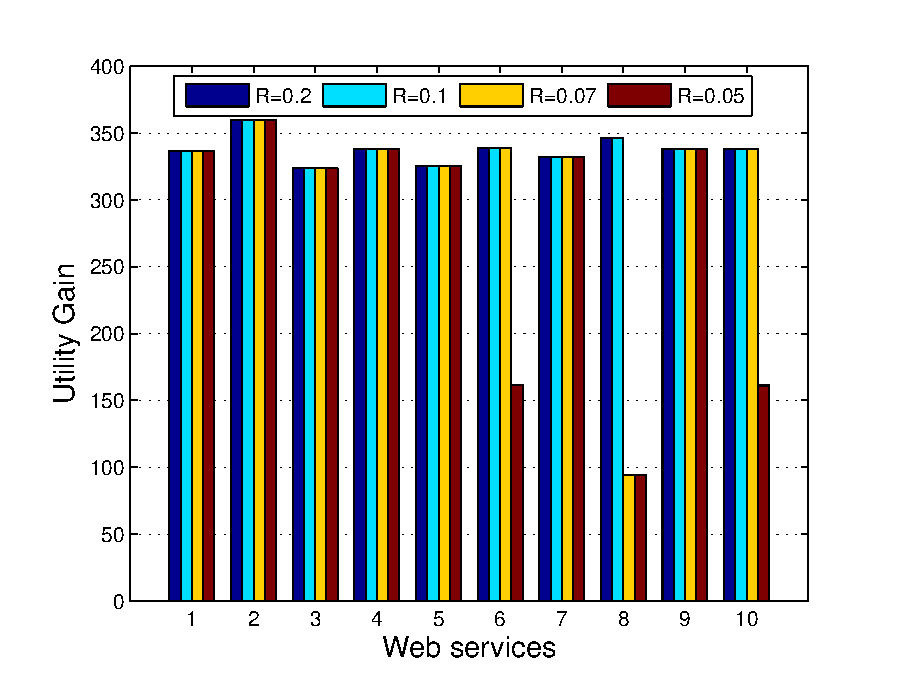
\includegraphics[width=3.5in]{figures/utility_gain_r.eps}
%\caption{DDM Utility Gain Value}
%\label{utility_gain_value}
%\end{figure}
%
%\begin{figure}%[!t]
%\centering
%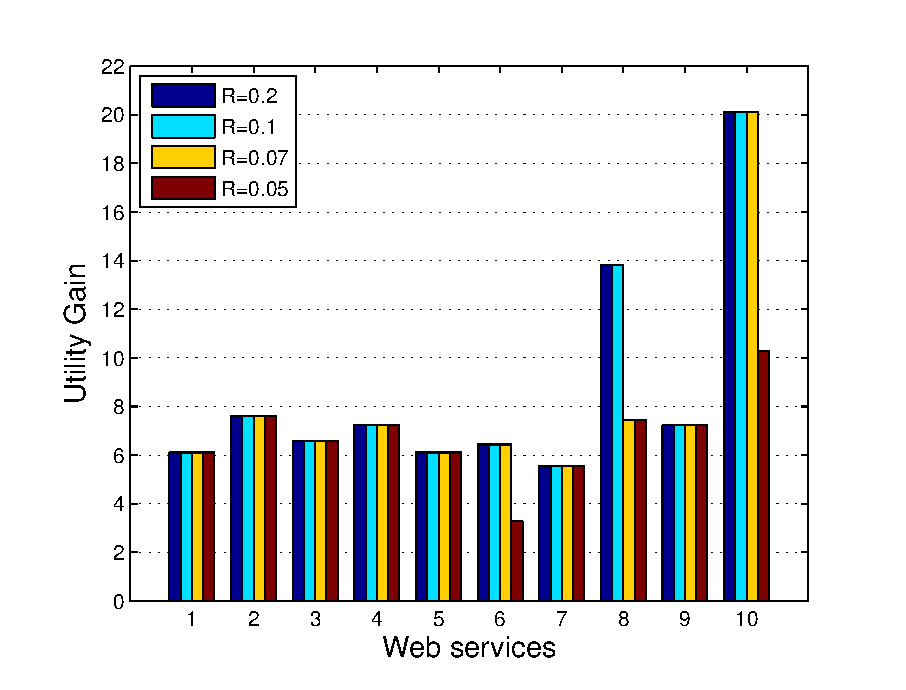
\includegraphics[width=3.5in]{figures/utility_ratio_r.eps}
%\caption{DDM Utility Gain Ratio}
%\label{utility_gain_ratio}
%\end{figure}


The closest related work \cite{10.1109/TSC.2012.12,
DBLP:conf/IEEEscc/LimTMB12, DBLP:conf/IEEEscc/KhosravifarABT11} and our
previous work \cite{journal-community-formation} regarding the community formation problem have considered a centralized approach where a community manager has complete information of all the web services and their quality
metric and parameters. Those proposals run complex algorithms through all the space of
solutions in order to find the optimal answer. However, in this research work, we
have considered an unexplored and more realistic situation where information is incomplete and a decision
profile is generated based on a smaller set of web services. Our solution helps
communities and web services select actions that lead towards
maximizing their utilities. Therefore, considering the different settings,
we cannot experimentally compare our work with the mentioned related work.


To compare our work against a benchmark, we utilize the same communities and web services with a simple rational decision making mechanism in which a community will choose to join another one if it increases its utility by any amount, without aiming to be optimal. We call this method the {\textit{rational} method. We have chosen 10 random web services and compared the results with web services which adopted our DDM model. Figure \ref{utility_gain_mlisa_and_rational} shows the comparison of the end result of utility gain values. In 18 out of 40 tries, \emph{rational} agents were not able to improve their utility at all because the communities they chose rejected their request, most likely because they would not have increased the utility of the other communities if they had joined them. The results show that a long-term strategic decision mechanism is needed to satisfy all the services within communities. Figure \ref{utility_gain_mlisa_and_rational_ratio} shows the same results in terms of ratio of utility gain.

\begin{figure}%[!t]
\centering
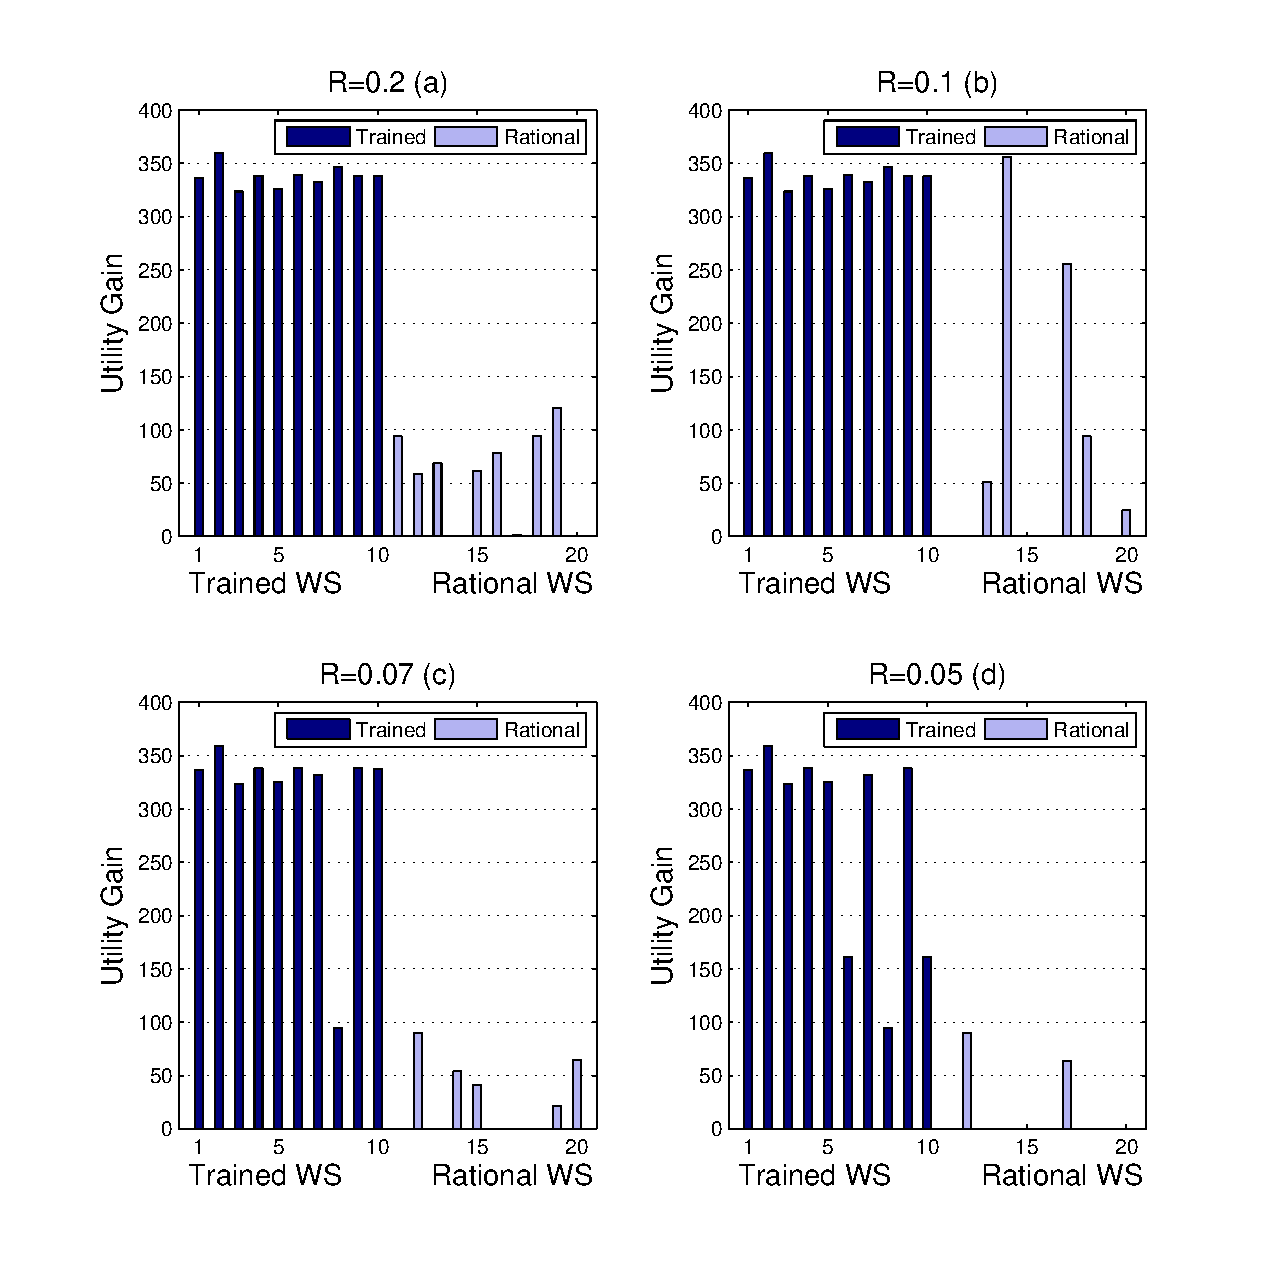
\includegraphics[width=5in]{figures/utility_gain.eps}
\caption{DDM against Rational: utility gain }
\label{utility_gain_mlisa_and_rational}
\end{figure}

\begin{figure}%[!t]
\centering
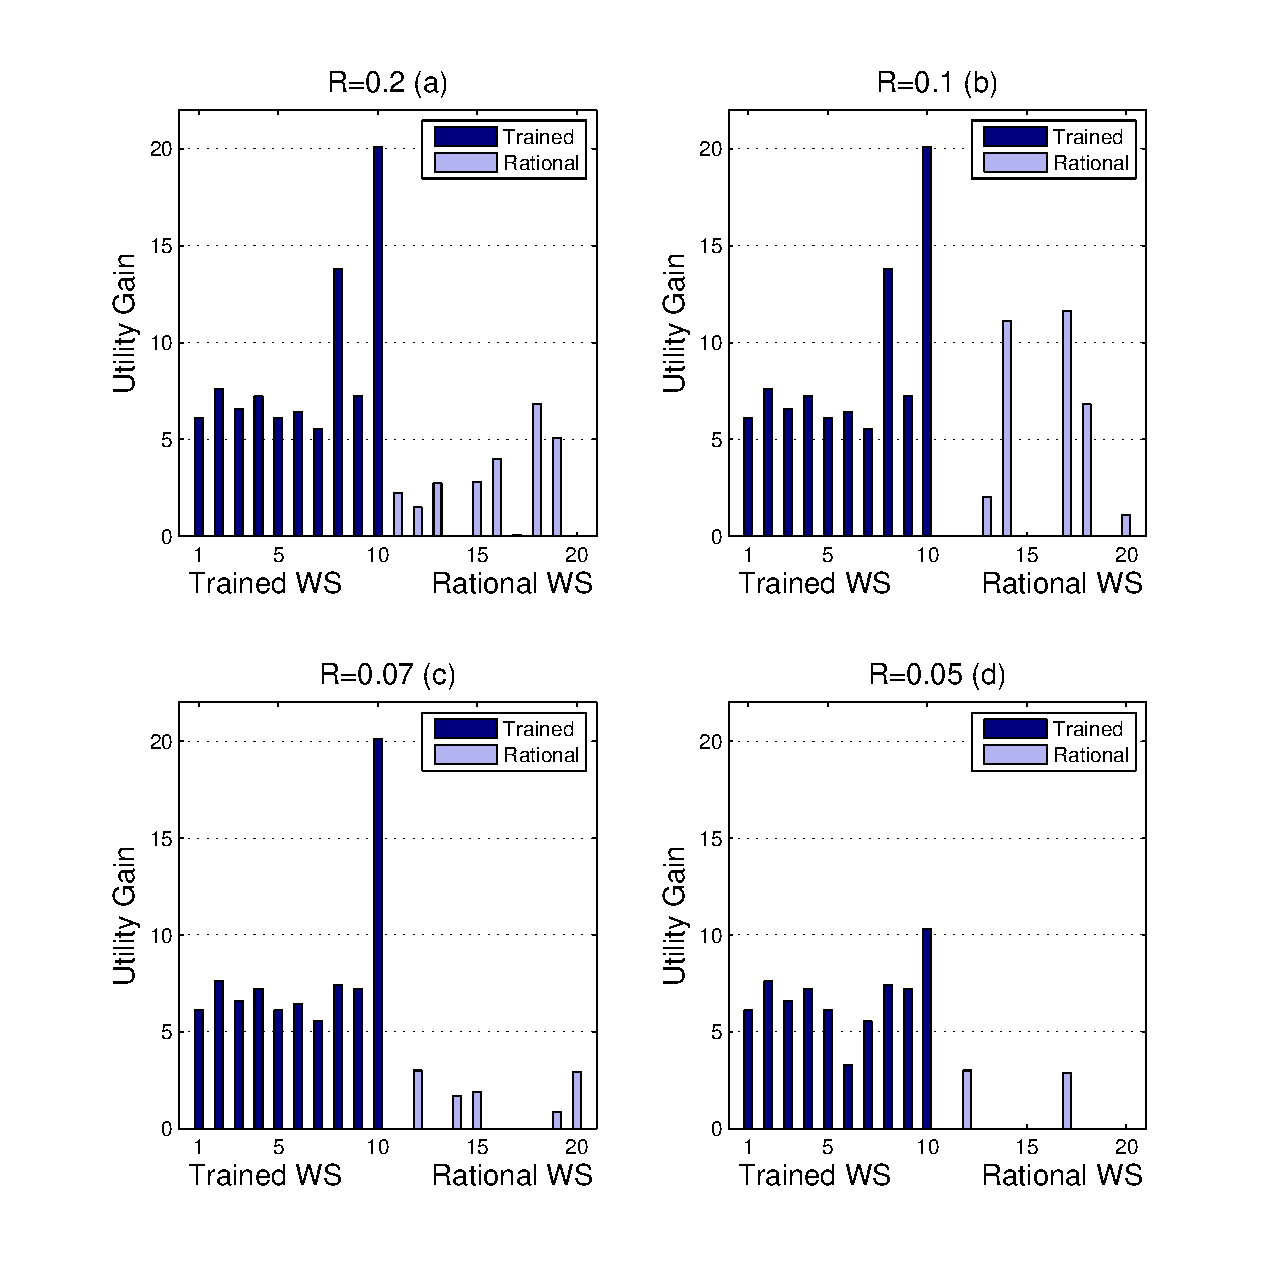
\includegraphics[width=5in]{figures/utility_ratio.eps}
\caption{DDM against Rational: ratio of utility gain}
\label{utility_gain_mlisa_and_rational_ratio}
\end{figure}

Now, we evaluate the performance of the decision profiles generated based on our data set for other communities.% which are not included in the decision tree creation process.
We create 1,000 communities from the web services in the data set that were not involved in the training process of our decision model. We define a distance function that measures the difference between basic features of communities, which measures the similarity among communities.

\begin{equation}\label{distance_c}
\begin{split}
distance (C_1, C_2) & = |Th_{C_1} - Th_{C_2}| \\
                    & + |A_{C_1} - A_{C_2}| + |Et_{C_1} - Et_{C_2}|
\end{split}
\end{equation}

Now, each community tries to find the closest community within the trained $CFVS$ set. Following its decision profile, the community can get a good estimate of the possible strategic decisions it can adopt. Basically, the trained profiles benefit the new communities in two ways. First, they provide the communities with a set of viable communities to join. Second, they provide an estimation of long-term utility gain for each available decision. In this experiment, we let communities follow the best decision within the decision tree provided to them.


In order to evaluate the performance of the mechanism, we used \emph{Receiver Operating Characteristic (ROC) curve}, which is a graphical plot illustrating the true negative rate against the false positive rate at various threshold settings in classifier systems. In order to classify our communities' selection strategies correctly, for each community, we evaluated the training process by replacing the community in the set with the closest one, from which it gets the strategy profile. If the actions are the same and the same utility levels are gained, we classify the decision as correct. Otherwise, it is classified as a wrong decision. \emph{AUC}, the area under the \emph{ROC curve}, is equal to the probability that a classifier will rank a randomly chosen positive instance higher than a randomly chosen negative one, and the higher the number the better the solution, which reflects better performance.  Figure \ref{roc5} illustrates the \emph{ROC curve} evaluation of the DDM decision making mechanism. As benchmark, we compare our method with two other methods: the \emph{rational} method and the \emph{greedy} method. The \emph{greedy} method only looks up the available list of communities and simply joins the community that maximizes its utility without considering any long-term strategy or other communities' acceptance scenarios. It is a greedy algorithm that focuses on choosing a locally optimal choice.

\begin{itemize}
  \item {\bf Rational Method:} Communities would send a join request to any available community, which will increase the utility. The other community would accept the join offer if its own utility gain is positive as well.
	\item {\bf Greedy Method:} Communities do a linear search among all the available communities and send a join request to the community which results in maximum utility. The other community would accept the join offer if its own utility gain is positive and the utility gain does not need to be the maximum for the community receiving the join request.
\end{itemize}

Figure \ref{roc5} compares the results for all the methods. The \emph{rational} and \emph{greedy} methods have very high failure rates compared to our method. Table \ref{fail_rate} illustrates the number of communities that failed to find the optimal collaboration group. The results support the need for a long-term training model in a successful decision making process.

\begin{figure}%[!t]
\centering
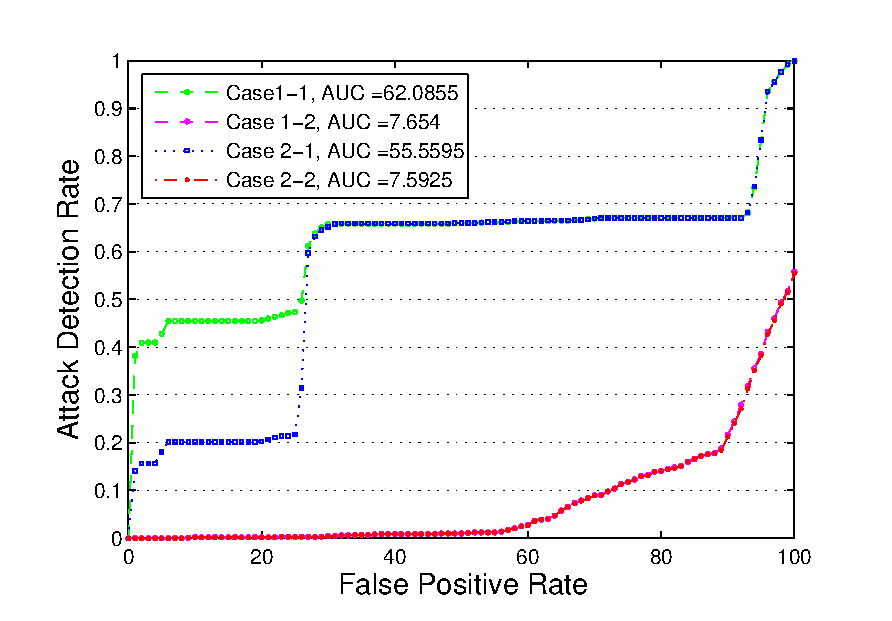
\includegraphics[width=4in]{figures/roc.eps}
\caption{RoC Curve}
\label{roc5}
\end{figure}

\begin{table}[ht]
\caption{Number of communities that misses the optimal decision, out of 1,000 communities} % title of Table
\centering % used for centering table
\begin{tabular}{|c|c|} % centered columns (4 columns)
\hline %inserts double horizontal lines
 Method&Miss \\ [0.5ex] % inserts table
%heading
\hline % inserts single horizontal line
 DDM r=0.05& 375 \\ % inserting body of the table
 DDM r=0.07& 137 \\
 DDM r=0.10& 6 \\
 DDM r=0.20& 6 \\
Rational Method& 717 \\
Greedy Method& 828 \\ [1ex] % [1ex] adds vertical space
\hline %inserts single line
\end{tabular}
\label{fail_rate} % is used to refer this table in the text
\end{table}


Now, we evaluate the system-specific results from users' and communities' perspectives. By distributing tasks among the communities over the 64 time frames, we evaluate the revenue for each community. Figure \ref{stats1} shows the overall revenue gain of communities using our method. Figure \ref{stats2} shows the momentarily revenue gain for each community in each time slot compared to the previous time. These results show that the run with the higher learning rate of $r=0.20$ starts discovering better communities to join much earlier. The runs with slow rates seem to find some communities to join initially, but then they slow down until later, when they start discovering new communities to join.


\begin{figure}%[!t]
\centering
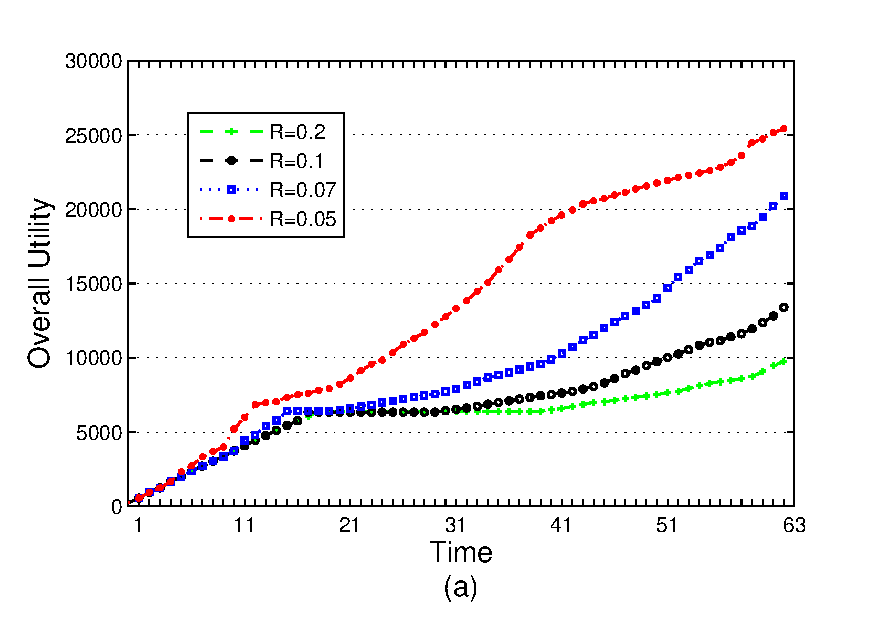
\includegraphics[width=4in]{figures/stats1.eps}
\caption{Overall utility of all the communities}
\label{stats1}
\end{figure}


\begin{figure}%[!t]
\centering
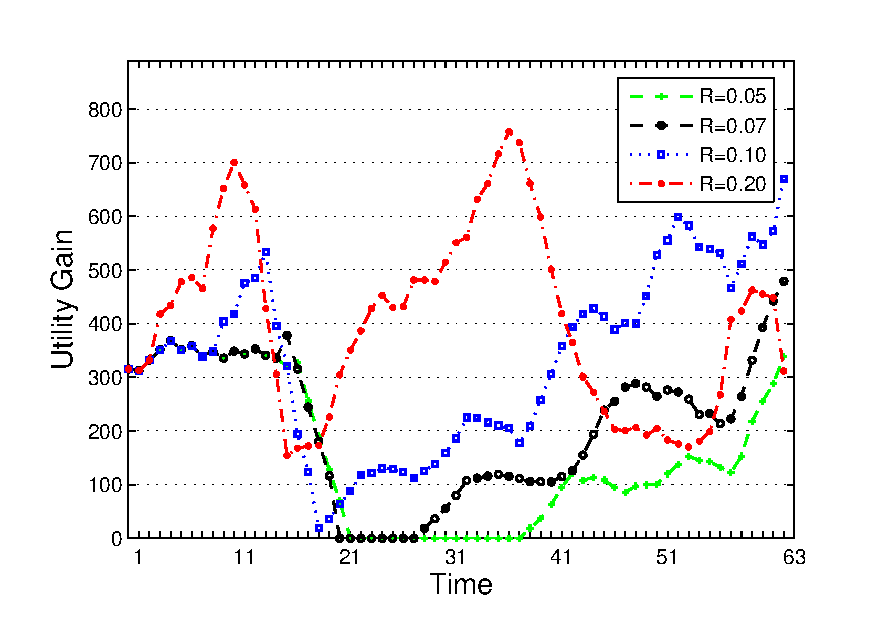
\includegraphics[width=4in]{figures/stats2.eps}
\caption{Utility gain over time}
\label{stats2}
\end{figure}

Figure \ref{stats3} depicts the average community size over time, which essentially represents the number of new communities being formed. The results show once again the communities using DDM with higher search rates grow faster in size, implying that the communities find appropriate web services to join with faster.

\begin{figure}%[!t]
\centering
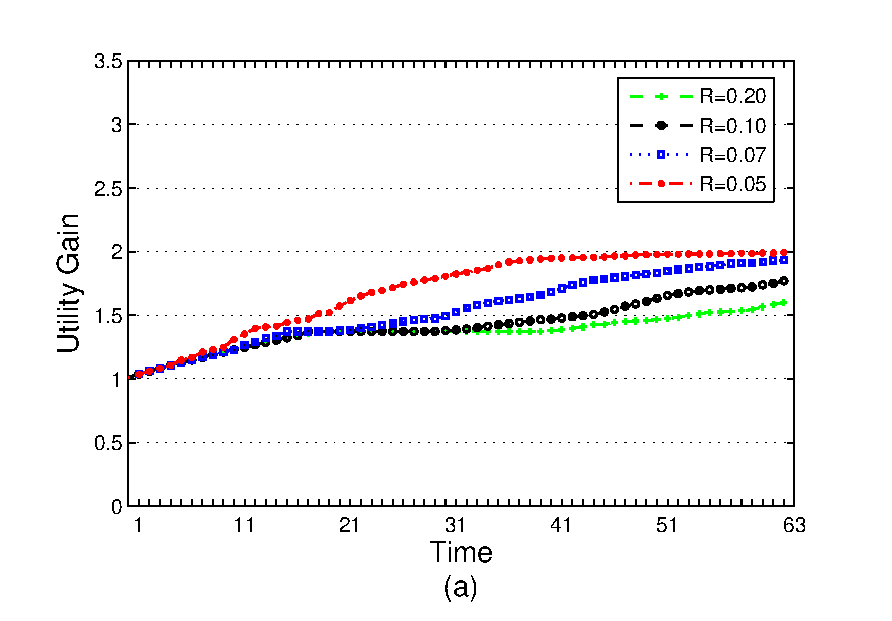
\includegraphics[width=4in]{figures/stats3.eps}
\caption{Average community size}
\label{stats3}
\end{figure}



%\section{Related Work}\label{s:related_work}
%
%Most of the recent work on communities of services are either
%user-centric and focus on user satisfaction
%\cite{Chun02user-centricperformance} or system-centric and focus
%on the whole system throughput, performance and utilization. There
%are many contributions in distributed, grid, cluster and cloud
%services which are system-centric. However, in real world
%environments and applications, both users and service providers
%are self-interested agents, aiming to maximize their own profit.
%In those environments, both parties (users and services) will
%collaborate as long as they are getting more benefits and payoff.
%
%In this direction, recently \cite{DBLP:conf/IEEEscc/LimTMB12,
%DBLP:conf/IEEEscc/KhosravifarABT11, 10.1109/TSC.2012.12} proposed
%mechanisms to help users and services maximize their gain. A
%two-player non-cooperative game between web services and community
%master was introduced in
%\cite{DBLP:conf/IEEEscc/KhosravifarABT11}. In this game-theoretic
%model, the strategies available to a web service when facing a new
%community are requesting to join the community, accepting the
%master's invitation to join the community, or refusing the
%invitation to join. The set of strategies for communities are
%inviting the web service or refusing the web service's join
%request. Based on their capacity, market share and reputation, the
%two players have different sets of utilities over the strategy
%profiles of the game. The main limits of this game model are: 1)
%its consideration of only three quality parameters, while the
%other factors are simply ignored; and 2) the non-consideration of
%the web services already residing within the community. The game
%is only between the community master and the new web service, and
%the inputs from all the other members and their influence on the
%master's decision are simply ignored. The consideration of those
%inputs and this influence factor is a significant issue as
%existing web services can lose utility or payoff because of the
%new member, which can result in an unhealthy and unstable group.
%The problem comes from the fact that the existing members should
%collaborate with the new web services, so probably their
%performance as a group can suffer. Existing members may even
%deviate and try to join other communities if they are unsatisfied.
%Those considerations of forming stable and efficient coalitions
%are the main contributions of our thesis.
%
%In \cite{DBLP:conf/IEEEscc/LimTMB12}, a 3-way satisfaction approach
%for selecting web services has been proposed. In this approach,
%the authors proposed a web service selection process that the
%community masters can use. The approach considers the efficiency
%of all the three involved parties, namely users, web services and
%communities. In this work, it is shown how the gains of these
%parties are coupled together using a linear optimization process.
%However, the optimization problem in this solution tends to
%optimize some parameters considering all web services regardless
%of their efficiency and contribution to the community's welfare.
%Moreover, there are no clear thresholds for accepting or rejecting
%new web services. The solution of the optimization problem could,
%for instance, suggest web services already residing within the
%community to increase or decrease their capacity to cover up the
%weakness of other parties in the system. However, a high
%performing web service could deviate anytime it finds itself
%unsatisfied within the community instead of adjusting its service
%parameters.
%
%In \cite{10.1109/TSC.2012.12}, a cooperative scheme among
%autonomous web services based on coalition game theory has been
%introduced. The authors have proposed an interesting algorithm to
%reach individually stable coalition partition for web services in
%order to maximize their efficiency. The communities choose new web
%services on the promise that it would benefit the community
%without decreasing any other web service's income. In the proposed
%model, the worth of community is evaluated with high emphasis on
%the availability metric and considering price and cost values
%only. The community structure is based on a coordination chain,
%where a web service is considered as a \emph{primary} web service
%and the community task-distribution method initially invokes the
%primary web service and only if the primary web service is
%unavailable, the method invokes the next backup web services as
%they are ordered in the coordination chain. We believe that this
%coordination chain limits the cooperation power as it introduces a
%sort of hierarchy. However, in pure and open cooperative models,
%such as the one we propose in this paper, active cooperation
%activities engaging simultaneously many agents so that they can
%perform the tasks more efficiently are being used. Moreover, if
%the availability is high, which is the case nowadays with the
%recent advancements in cloud infrastructures and hardware technologies, the
%backup web services will end-up having a very low chance of
%getting jobs, especially the ones further in the chain. This will
%results in a considerable waste of web services capabilities.
%
%All the proposed frameworks share a common aspect, which is providing the solution based on assumption of having complete information of all services and performing evaluations based on a large number of input each time they want to adopt a strategic decision making process.
%So basically, these solutions generally suffer from high complexity, which makes decision making very hard, even impossible in some cases in a real-time fashion, or they simplify important aspects to make it practical in the real world, thereby hurting the decision making performance. We address this issue by introducing DDM a framework that operates based on a trained model that regulates web service agents' decision making process in terms of cooperating with one another. After being trained, web services get to compute expectations as utilities they would gain while cooperating with communities of different characteristics. Therefore, web services and communities can make prudent decisions when inviting a web service to join or accepting a join inquiry initiated from a web service. In general, DDM equips web services with efficient methods for foreseeing how their choices will impact their long-term and short-term goals; therefore, opting for best decision available. \\
%
%\noindent \textbf{Web Services Communities}
%
%Here we introduce the related research work regarding the engineering and formation of communities of web services. In \cite{DBLP:journals/internet/BenatallahSD03}, Benatallah et al. defined communities of web services as \emph{Service Containers} that aggregate substitutable web services having the same set of operations and providing common functionalities. They abstracted \emph{Service Containers} as web services that are created, advertised, discovered and invoked just as elementary web services. The \emph{Container} is considered as a manager that is responsible for web service selection upon receiving a request on run-time. The authors have proposed a scoring technique based on non-functional requirements of the request and web service capabilities to dynamically chose the web service to perform the requested task. A similar concept was proposed by Maamar et al. in \cite{DBLP:journals/ijebr/MaamarSTBB09}. The authors introduced web services communities as a collection of web services with a common functionality but different QoS properties. A community manager, upon receiving a request, delegates the request to one of its current members. The choice is based on the performance history and quality metrics of each web service. The authors have proposed an efficient global web service selection algorithm in order to approach quality constraints and preferences for composite services which requires aggregation of different types of services to satisfy the user. In the same line of research, Benslimane et al. \cite{Liris-2770} have proposed a multi-layer approach grouping similar web services into communities and having an interface implemented as an abstract web service for accessing the community. The considered layers are: composite, management and community. The interactions among those layers and the bindings are performed by a generic driver called Open Software Connectivity (OSC). However, unlike our work, these proposals only tackle the problem of internal community management from the task execution perspective, but not the problem of community formation and the one of dynamically selecting which community to join and which web service to invite. Moreover, the web services selection process is done centrally by the community manager, while we address the problem more realistically from the distributed angle.
%
%In \cite{managing-hela-jalel}, Limam and Akaichi have proposed web
%service communities with centralized access across distributed web
%services. They have proposed a framework for web service
%management, query resolution among communities and a query caching
%mechanism executed by the manager to improve the performance of
%query resolution process among many distributed communities. The
%key idea is to cache previous computed results for answering
%future queries. Maamar et al. initially in \cite{conf/webist/MaamarLBTS07} and
%then comprehensively in \cite{DBLP:journals/ijebr/MaamarSTBB09}
%proposed an architecture utilizing \emph{Contract-Net} protocol
%for engineering task distribution within communities of web
%services. The protocol is centrally executed by the community
%manager. This architecture has been further extended in
%\cite{CSTintercommunity, conf/IEEEscc/BenharrefSBB11,
%conf/IEEEscc/KhosravifarBMMT10, conf/aina/LimTM11}. Two types of
%roles have been distinguished for community members: masters and
%slaves. Master web services are community managers that lead
%communities and are responsible for membership management. They
%can invite and convince slave web services to join the community,
%and attract new slave web services to their communities by
%awarding them better payoff. Moreover, they can eject some slave
%members from the community to improve its overall reputation if
%these members are misbehaving or cannot provide the promised QoS.
%In \cite{Medjahed05adynamic}, Medjahed and Bouguettaya have
%developed a community as a ``cluster'' that groups Web services
%based on a specific area of interest. All web services in a given
%community share the same functionality. These communities are
%created by \emph{third party community providers} which use the
%\emph{community ontology} as a template and define a set of
%operations that all web services within a community should
%provide. Using semantic analysis on web service operations, web
%services either find and join a community with similar
%functionality or create a new operation description for a new
%community. The authors have described the concept of
%\emph{community agents} associated to \emph{community providers}.
%A community agent is responsible, among other things, of the
%registration of services with the community. An example of a
%community that provides health care services to senior citizens
%has been used. In this example, a governmental entity is needed to
%check the health care standards used by the members before
%authorizing them to be part of the community. Such a central
%entity is represented by the community agent. Thus, community
%agents are playing the role of community managers. In a close work
%\cite{Zeng:2003:QDW:775152.775211}, Zeng et al. have described a
%global planning selection algorithm and a delegation algorithm to
%be run when a request to execute an operation is received by the
%community. This needs a central entity to run those algorithms.
%Such entity plays the same role as the community coordinator or
%manager. All these proposals have in common the consideration
%of the central entity for community management, which includes the hiring and firing of the community members, while our approach is fully distributed. Moreover, the stability of the community has not been investigated. Another major difference with our work is that the decision making process is only one way and unilateral from the community manager perspective. In our contribution, both participants, namely communities and web services, participate in the decision making process and a joining decision is made only if it is the best option for both players.


%%%%%%%%%%%%%%%%%%%%%%%%%%%%%%%%%%%%%%%%%%%%%%%%%%%%%%%%%%%%%%%
\section{Summary}\label{sec:conclusion-cha4}

In this research work, we proposed a training model for the problem of membership management of communities of web services. Using the traning model we created a decision making profile for each community and web service involved which provides them with a set of feasible and utility increasing moves. This utilized our web services with efficient methods of foreseeing how their choices of actions would impact their long-term and short-term goals, therefore they opted for best decision available. The ultimate goal is to choose the best decision when it comes to communities formation, among many possible short-term rational and utility increasing choices. The experimental results show that our algorithms provide web services and community owners, in real-world-like environments, with applicable and near-perfect decision making mechanisms. The results of experiments using real data samples support the need for a long-term training model in a successful decision making process.

%Our plan for future work is to advance learning process on the training set that we provided in our work. SVN machine learning algorithm are suitable in classification of our training data set, to better classify correct or wrong decisions based on long-term utility gains, as data set outputs. This can further facilitate the process of finding optimal cooperators in regards to enhancing web services' overall performance as service providers.

In next chapter, we analyse the internal community behaviour of web services, and propose a model for competing and cooperating agents within the communities of web services.



%%%%%%%%%%%%%%%%%%%%%%%%%%%%%%%%%%%%%%%%%%%%%%%%%%%%%%%%%%%%%%%%%%%%%%%%%%%%%%%
%% Chapter 5 : Probabilistic Group Social Commitments.
%%%%%%%%%%%%%%%%%%%%%%%%%%%%%%%%%%%%%%%%%%%%%%%%%%%%%%%%%%%%%%%%%%%%%%%%%%%%%%%
\setcounter{chapter}{4}

\chapter{Distributed Decision Making for Dynamic Formation of Web Services Communities}\label{cha:PCTLKC}


\section{Introduction}

Over the past years, online services have become an important part of many scalable business applications. The increasing reliance on online service providers has significantly influenced the way web services are engineered. Given the dynamic and unpredictable nature of the Internet, delivering high quality services is still a critical and challenging issue. One practical solution towards delivering such quality services is utilizing intelligent decision making agents. These agents aim at maximizing their gain by exploring the best ways to provide services that satisfy end users \cite{Zeng:2003:QDW:775152.775211, 10.1109/ARES.2008.7, Demirkan2013412, journals/tsc/ZhengZYB13, Josang:2007:STR:1225318.1225716}. However, agent-based web services are functionally limited in the sense that they cannot handle a large number of requests at the same time without compromising the quality of service provided. Recent developments have attempted to shift web services from simple models, consisting of individual components, to models made up of autonomous and group-based components that share common goals. In group-based models, interaction, composition, and cooperation are the key challenges that directly impact the group's overall performance in achieving common goals \cite{ICWS2011-1, SCC2011-1, journals/mags/BaldoniBM10, journals/jcss/CasadoYT13}. To that end, we see the emergence of web service \emph{communities}, which consist of grouping services with similar functionalities but distinct nonfunctional properties \cite{Zeng:2003:QDW:775152.775211, 10.1109/ARES.2008.7, Paik:2005:TSS:2229263.2230038, Medjahed05adynamic}. A community of web services runs continuous performance assessment functions that regulate web services' interactions and manage their composition and cooperation.

Web Service communities have the advantages of facilitating web service discovery and providing better quality of service compared to individual services. Communities act as abstract web services, communicating with external entities via the same standard protocols that a normal web service employs. The difference is that communities regulate the service process via sophisticated internal communication protocols, thereby providing services based on the combined efforts of a number of web services. The downside to communities is the complexity of management involved in finding and inviting adequate individual services and managing the overall quality of the combined work of several services.
% because although they have similar functionality, they have different attitudes.
When interacting with a community of web services, users send their requests to the coordinator of the community, which plays the role of community representative or access point. The community coordinator is responsible of receiving tasks and delivering services. Moreover, as community representative, it verifies the credentials of new web services before accepting them into the community and kicks services that could harm the value of the community.

\textbf{Challenges and Problem Statement.} In recent work, communities of web services have been proposed in order to facilitate discovery of web services, improve the Quality of Service (QoS), and help individual services find better market share and opportunities \cite{Zeng:2003:QDW:775152.775211, 10.1109/ARES.2008.7, Paik:2005:TSS:2229263.2230038, Medjahed05adynamic}. However,  two important challenges are to be addressed: 1) choice of the best web services during community development from the community perspective; and 2) choice of the best community to join from the web service perspective. The advocated solutions  \cite{10.1109/ARES.2008.7, conf/webist/MaamarLBTS07, journals/soca/XuYLZB11, 10.1109/TSC.2012.12, managing-hela-jalel, DBLP:conf/IEEEscc/KhosravifarABT11, DBLP:conf/IEEEscc/LimTMB12} have attempted to address these challenges. However, those solutions have two main limits:
\begin{enumerate}
	\item The solutions consider the architecture of centralized management for communities where most of the decisions are made by the centralized coordinator. The problem is that in real world scenarios, decisions made by independent service providers are highly distributed.
	\item The solutions either propose complex algorithms \cite{10.1109/TSC.2012.12, DBLP:conf/IEEEscc/LimTMB12, journal-community-formation} to find the optimal strategy to follow, or oversimplify the problem by eliminating important parameters and using approximation techniques to make the algorithms tractable \cite{10.1109/TSC.2012.12}.
\end{enumerate}
These approximation methods sometimes negatively influence the outcome because simplifying the constraints may cause important aspects of the problem to be ignored. For instance, instead of calculating the gain distribution using the adequate, but complex shapely-value method, the authors is \cite{10.1109/TSC.2012.12} propose a simple egalitarian way of distributing gain, which completely ignores the gain generated from collaborative work of sub-communities. Other categories of related work, for instance \cite{10.1109/TSC.2012.12, DBLP:conf/IEEEscc/KhosravifarABT11, DBLP:journals/ijebr/MaamarSTBB09}, restrict the decision process within the community coordinator, so other members of the community are not effectively involved.
%And some other work which do not focus on rationality on web services or communities involved [refrences].
In \cite{journal-community-formation}, we proposed a cooperative game-theory-based model for aggregating web services in communities. A centralized decision maker in communities, based on a complete knowledge of available web service quality metrics and performance, has been used to form optimal and stable communities that maximize individual and group income. However, centrality and complete information are strong assumptions, which are not very compatible with real business scenarios.

\textbf{Contributions.} In this paper, we introduce DDM, a Distributed Decision Making model for community formation that regulates web service agents’ decision making process in terms of cooperating and deciding which group to join and which service to invite for joining. Unlike existing work on community formation, our decision model is extracted from a data model in the form of information obtained from a large number of web services regarding their single and cooperative utilities as well as environmental parameters such as demand, service quality, etc. The generated decision tree improves agents' understanding of the environment and how to select actions that lead towards maximizing their utilities. The advantage of this approach is that the tree, which is initially created from the past data, reflects a comprehensive vision about agents' attitudes in terms of their action selection based on their past experiences. Moreover, the tree is getting continuously updated based on both new received feedback and the outcome of chosen actions. This continuous update makes the approach adapted to any change in the environment.
%The training model deploys a logistic regression algorithm to build a hypothesis function that can thoroughly address the aforementioned research problems.
The decision model provides web services with enough information which helps those services efficiently decide and predict the outcome of their different possible collaborations. This model works in a distributed manner in which services are self-sufficient in their decision making and do not rely on a centralized decision making process. Our findings show that communities of web services can efficiently find the appropriate web service to invite for cooperation as well as allowing a single web service to find the best communities to join. The proposed model can be seen as a recommneder system that suggests beneficial actions for both communities and single services. Communities can consider the decision model and analyze the characteristics of different individual web services and make prudent decisions when inviting a web service to join or accepting a join inquiry initiated from a web service. In general, DDM equips web services with efficient methods for foreseeing how their choices will impact both their short-term and long-term goals; therefore, opting for the best decision available.

To effectively generate the decision model for web services, we used a real dataset to extract web services' individual characteristics and used them to measure outcomes when these services cooperate with one another. The dataset has been extracted from real-world QoS evaluation results from 142 users on 4,532 Web services during 64 different time slots. Combining the available data based on each web service point of view on different time slots, we acquired 5 different unique features for those 4,532 web services. By engineering and extracting these features, we gathered functional and cooperative features for both individual web services and communities in different time slots. We were able to investigate the path a web service might take to achieve the best utility out of effective interactions with others. All the paths and outcomes are labeled to be utilized in the training model. Using cross validation sets, web services are able to compute the optimal hypothesis function (using logistic regression) that can be used to predict outcomes of cooperative work with other individual web services or communities. Our findings show that web services equipped with DDM have by far better outcomes than the ones that either do not cooperate or randomly find communities to join.

\section{Preliminaries and Challenging Issues}\label{s4:preliminaries}
%In this section, we first present the architecture of DDM. We explore the characteristics of intelligent service agents and the features we extract for training. To do this, we first discuss some preliminaries.
In this section, we discuss the preliminary concepts of communities of web services and introduce the challenges behind community formation.

\subsection{Web Services}\label{s:ws}

In the recent years, online services have become a standard part of daily life around the globe. Many modern applications rely on web services from different providers. For instance, many mobile and tablet applications that have limited storage and processing power are merely aggregating information from different online services. Examples are vast, including weather forecasting, ticket selling, shopping apps, local maps and location services.

The World Wide Web Consortium (W3C) defines web services as ``software systems designed to support interoperable machine-to-machine interaction over a network. It has an interface described in a machine-processable format (specifically WSDL). Other systems interact with the web service in a manner prescribed by its description using SOAP messages, typically conveyed using HTTP with XML serialization in conjunction with other Web-related standards''. When developers declare a new web service, it will be
discovered based on its description, which fully discloses its functionalities. Developers also have to declare a public interface and a readable documentation to help other developers when integrating different services \cite{w3cwsdl}. Nowadays, web API, standards that do not require XML-based web service protocols like SOAP and WSDL are also emerging. They are called RESTful (representational state transfer) services, which are moving towards simpler communication protocols.
%They are not restricted
%to XML formats, recently JSON, a human readable and simpler format
%is becoming popular among online service providers.

We are not going to delve into the engineering details of online web service implementation and its protocols in this paper. We are interested in web services from a business model perspective. Service providers usually charge end users for services they provide. For example, Google has listed pricing and plans for a wide range of services they provide on their web service console page\footnote{$https://code.google.com/apis/console$}.

As in other proposals \cite{journals/mags/BaldoniBM10,10.1109/TSC.2012.12,DBLP:conf/IEEEscc/KhosravifarABT11}, in this paper, we abstract web services as rational agents\footnote{The term rational is used here in the sense that web services are utility maximizers.} that provide services to end users. They aim to maximize their individual income  by receiving enough requests from end users. In order to increase their revenues, web services seek for more tasks if they have the capacity and throughput to do so. Web services can join communities to enhance efficiency by collaborating with others, to have access to broad market share, and for the opportunity to receive a bigger task pool from end users.
Furthermore, the high reliance on web services has resulted in increased quality expectations from end users. Communities of web services can provide higher availability, performance, reliability, and recovery for end users.

\subsection{Web Service Communities}\label{s:wsc}

The community of web services is essentially a virtual group of web services having similar functionalities \cite{DBLP:journals/ijebr/MaamarSTBB09}. Communities aggregate web services and communicate with other entities such as UDDI registries and users, using identical protocols to those used by single web services. Web services join communities to increase utility by having a larger market share and task pool. The community coordinator is responsible for securing the community, managing membership requests from web services and distributing user tasks among the community members. The coordinator tries to attract quality web services to join and keep the community as stable and productive as possible to gain better reputation and user satisfaction, which increases the community's market share. How web services reside within communities and how communities of web services are engineered is described comprehensively in \cite{DBLP:journals/ijebr/MaamarSTBB09}.

\subsection{The Join Challenge}\label{s:tjc}
It has been showed in \cite{10.1109/ARES.2008.7,10.1109/TSC.2012.12,journal-community-formation} that web services can increase their overall utility by collaborating with other web services within communities. This collaboration provides them with better ways of sharing resources and having higher reputation, greater market share and wider visibility. Web services and communities come with different quality metrics, and the long-term outcome depends on these metrics.

The goal of all parties involved in the community is to maximize their long-term outcome while they are operating as part of the community. Web services need to be equipped with a selection strategy to choose from the different possible collaboration groups they can form as well as an estimation method for evaluating the long-term gain of joining different possible communities. Web services need to experiment with different possible collaborative groups in order to estimate their gain over time. However, with a high number of possible communities, it is not possible to test collaboration with random web services. Even if a linear approximate function for estimating utility based on community web services' parameters is adopted, the exponential \footnote{Bell number: $http://en.wikipedia.org/wiki/Bell\_number$} growth rate of the possible number of partitions of web services into communities would make any brute-force type algorithm for the best community selection strategy intractable and impractical in real-world application settings.

\subsection{Join Consequences}\label{s:jc}
It is worth mentioning that a \emph{join} event takes place as a result of interaction between two parties that are looking to expand their collaborations. All actions are chosen in an attempt to enhance the overall outcome. However, the selected action may result in decreasing the overall utility in the long run.
% long term.
This is the case when a single web service joins a community, but the complex process of task allocation eliminates the visibility of that service, which stays idle within the community. This makes the join action of that service a bad decision. The same event might be beneficial for the community, as it hosts a new web service that can engage in performing a new coming task. But overall, in this particular case, if the new web service stays idle for a long period of time, neither side will benefit from collaborating with the other and the join event will result in negative consequences for at least one side's utility.

The more common scenario is when both parties benefit from the joining of a web service to a community. This joining action is then rational as both the web service and community enhance their utilities. However, the community may not be the best choice for the web service. In other words, the web service could have joined a better community if it had enough and accurate knowledge about the surrounding environment. Since the community does enhance its utility, the web service could stay with that community, which results in a non-optimal increase in web service's utility. In the following section, the proposed model provides solutions that effectively address the aforementioned challenges.

\section{The Model Components}\label{s:themodelcomponents}

In this section, we discuss the parameters that we use in the rest of the paper. Then, we present the task distribution and revenue model of our distributed web services communities.

\subsection{Internal Features}\label{s:if}

With a group of web services having identical or similar functionalities, QoS metrics provide nonfunctional characteristics for optimal candidate selection. Web services quality metrics have been studied and analyzed in various proposals, for instance in in \cite{Ardagna:2007:ASC:1263152.1263531,Menasce:2002:QIW:613357.613758,10.1109/ISSRE.2011.17}. In this paper, we adopt the most representative QoS properties of those services that highly influence their utility.
%We refer to a typical web service as ws_{i}.

Let $C = \{ws_1,ws_2,..., ws_n\}$ be a community with $n$ web services. We define the following features for the group of web services based on their functional parameters:

\begin{itemize}

  \item \emph{Throughput} is the rate at which a service can process requests. QoS measures can include the maximum throughput or a function that describes how throughput varies with load intensity. Throughput is a positive real number. For a given community $C$, the expected throughput value $(Th_{C})$ can be estimated as the summation of throughput of all the service members $Th_{w}~ (w \in C)$:
	
	\begin{equation}
		 Th_{C} = \sum_{w \in C}{(Th_{w})}
	\end{equation}
	
	\item \emph{Availability} is the percentage of time that a service is operating. It is computed as
the probability that the service operation is accessible. Availability of a web service $A_w$ is a real number in the range $[0, 1]$. For a community $C$, the expected availability $(A_{C})$ considering the members operate in parallel (independently from each other) can be estimated as:
	
	\begin{equation}
		A_{C} = 1-\prod_{w \in C}{(1-A_{w})}
	\end{equation}
	
	\item \emph{Execution Time} is the time a service takes to respond to various types of requests.
	%is the expected delay between the time instant when a request is sent and the time when the result is obtained.
	Execution time is usually measured in milliseconds and can be affected by load intensity, which can be measured in terms of arrival rates (such as requests per second) or number of concurrent requests. This internal feature is a positive integer. For a typical community $C$, the expected execution time $Et_{C}$ can be estimated as the execution time of the bottleneck service which is the service with the slowest execution time $Et_{w}$:
	
	\begin{equation}
		Et_{C} = max_{w \in C}{(Et_{w})}
	\end{equation}
	
	%\item \emph{Data Quality} The ability of a data collection to meet user requirements , defined as the proximity of a value v returned by web service to a value considered as correct. The measure of data quality is considered here as a real number in the range [0, 1], where 1 represents the most desirable score.
\end{itemize}


	We normalize the range of these features so that each feature contributes proportionally to the final utility outcome value. We adopt the \emph{standardization} method consisting of subtracting the \emph{mean} from each feature, then dividing the subtraction result by the \emph{standard deviation}.

%$HI = \overline{HI}$

\subsection{External Features}\label{s:ef}

The quantitative values of quality metrics need some benchmark values to represent their goodness. In fact, without some benchmark values, it would be difficult for web services to identify their performance quality at any specific value of these metrics. Therefore, we introduce two external features for assessing web services' estimate with regard to their standing among other web services.

\begin{itemize}
  \item \emph{External Parameter 1} ($Exp1_i$ where $i$ is a community or a web service) is an estimate of how close the community's or the web service's \emph{execution time} is to the best execution time in the whole system. It is the difference between a community's or a web service's \emph{execution time} metric and the minimum value of execution time of all the other communities or web services. The smaller the value the better the external feature compared to other peers. In other words, small value of $Exp1_i$ means $i$ is among the best communities or services in the system.
	\begin{equation}\label{exp_1:f}
		Exp1_i = Et_{i} - Et_{min}
	\end{equation}
	\item \emph{External Parameter 2} ($Exp2_i$ where $i$ is a community or a web service)  is a comparison of the community's or the web service's rate of performing tasks to the best rate in the system. It is the difference between a community's or a web service's \emph{throughput} metric and the maximum value of throughput in the system. As for $Exp1_i$, the smaller the value the better the external feature.
	\begin{equation}\label{exp_2Lf}
		Exp2_i = Th_{max} - Th_{i}
	\end{equation}
\end{itemize}

\subsection{Task Distribution}

Communities of web services usually employ an implementation of Contract-Net protocol for task distribution, in which services bid on incoming tasks, and receive some of the tasks for which they bid \cite{DBLP:journals/ijebr/MaamarSTBB09,DBLP:conf/aina/ElnaffarMYBT08}. In our model, our community members would try to distribute tasks based on their capabilities and the QoS parameters provided by the web services. We use a slightly modified \emph{weighted fair queuing} method to distribute tasks among community members. The goal is to allocate incoming tasks to web services with a rate matching the throughput value of $Th_{w}$ for each web service $w$. In the \emph{weighted fair queuing} method, the input flow is multiplexed along different paths. However, in our model, if the rate of incoming tasks is less than the community's total throughput $(Th_{C})$, which is the summation of throughput values of the web services in the community, some of the input tasks will be queued and served with a delay.
%Thus, the amount of tasks performed by the community is $\sum_{ws}{Th_{ws}}$ when $\sum_{ws}{Th_{ws}} \leq R_{C}$.
When the incoming task rate is less than the throughput of the community, the \emph{weighted fair queuing} algorithm assigns a weighted task rate of $Itr \times \frac{Th_{w}}{\sum_{w}{Th_{w}}}$ for each web service $w$ within the community, where $Itr$ is the input task rate.

While distributing tasks, the community can verify the performance, throughput and quality of service of tasks being performed by web services. The community can assess if those web services are capable of performing the number of tasks they advertised. If for any reason, there is a decline in the quality metric or throughput, the community can consider the new values as a benchmark for future performance calculations, and penalize the suspicious web services. This way, players will have incentive to truthfully disclose their actual capabilities in order to maximize profit from the community and to avoid being penalized. In addition, the system should be dynamic enough to detect and react to web services' quality metrics variation, as over time, web service metrics may degrade or improve, changes to which the community should adjust.
% Therefore its easy for the system to encourage players to be in some sense incentive compatible in the way that they would profit best by truthfully revealing their capabilities. Also it is important to be dynamic enough to consider web services which may have their quality metrics degraded or even improved over time for any reason and be able to adjust the community with new parameters.

\subsection{Community Revenue}

Communities and web services earn revenue by performing tasks. The total gain is a function of the quality and rate of performing tasks. The utility of a collaborative group of services $U_{C}$ (i.e., the revenue of the community) is a function of internal and external parameters:

\begin{equation}\label{u_c_general}
U_{C} = f(A_{C}, Et_{C}, Exp1_{C}, Exp2_{C}, Th_{C})
\end{equation}
%
where $f$ is increasing in $A_{C}$ and $Th_{C}$ and decreasing in $Et_{C}, Exp1_{C}$ and $Exp2_{C}$. An example of this function is given in Equation \ref{u_c_normal}:

\begin{equation}\label{u_c_normal}
U_{C} = \big((\alpha \times (A_{C} - Et_{C}) - \beta \times (exp1_{C} + exp2_{C})\big) \times Th_{C}
\end{equation}

The $\alpha$ and $\beta$ parameters are internal and external weight coefficients. Small values for execution time and external parameters ensure better performance, which justifies their negative coefficients. The result is then multiplied by the throughput value $Th_{C}$, since communities are performing tasks with $Th_{C}$ rate.

\begin{theorem}
The function given in Equation \ref{u_c_normal} satisfies the properties of $f$.
\end{theorem}

The proof of this theorem is straightforward by simply calculating the partial derivative $\partial f$ with respect to the different variables.


The estimation of the utility can be improved, especially in cases where the input task rate is high and services are experiencing high task loads. The \emph{weighted fair queuing} method of task distribution would distribute tasks based on the individual throughput $(Th_{w})$ value of services within community. In fact, services having higher throughput affect strongly the overall utility of the community because they would take on proportionality more tasks. The improved utility is given as a function of individual internal and external parameters:


\begin{equation}\label{improved_u_c_general}
U_{C} = g_{w\in C}(A_{w}, Et_{w}, Exp1_{w}, Exp2_{w}, Th_{w})
\end{equation}
%
where $g_{w\in C}$ is increasing in $A_{w}$ and $Th_{w}$ and decreasing in $Et_{w}, Exp1_{w}$ and $Exp2_{w}$. An example of this function is given in Equation \ref{u_c_load}:


\begin{equation}\label{u_c_load}
\begin{split}
U_{C} = \sum_{w \in C}&\bigg(\big(\alpha \times (A_{w} - Et_{w}) \\
        & - \beta \times (Exp1_{w} + Exp2_{w})\big) \times Th_{w}\bigg)
\end{split}
\end{equation}

The following theorem holds:

\begin{theorem}
The function given in Equation \ref{u_c_load} satisfies the properties of $g_{w\in C}$.
\end{theorem}


\section{The Decision Making Mechanism}\label{s:model}

In this section, we describe our data extraction process and the methodology used to equip web services and communities with a decision making mechanism. In this methodology, we first present the data extraction and engineering process and then we evaluate the decision making mechanism for web services in community settings. Figure \ref{fig_steps} summarizes the steps performed in DDM from the input data to the generation of decision making profiles for web services and communities. The objective is to use the input data to build a decision tree for each service and community included in the data set, which will be be served as a benchmark for other services and communities in their decision making mechanism. The decision tree is made up by training the real data obtained from operating web services and extracting features related to their performance, either alone or as part of a joint effort with other web services. The ultimate objective is to propose for each web service and community the best joint decision about forming a group that maximizes every one's utility. The DDM's steps are explained in the following sections.

\begin{figure}%[!t]
\centerline{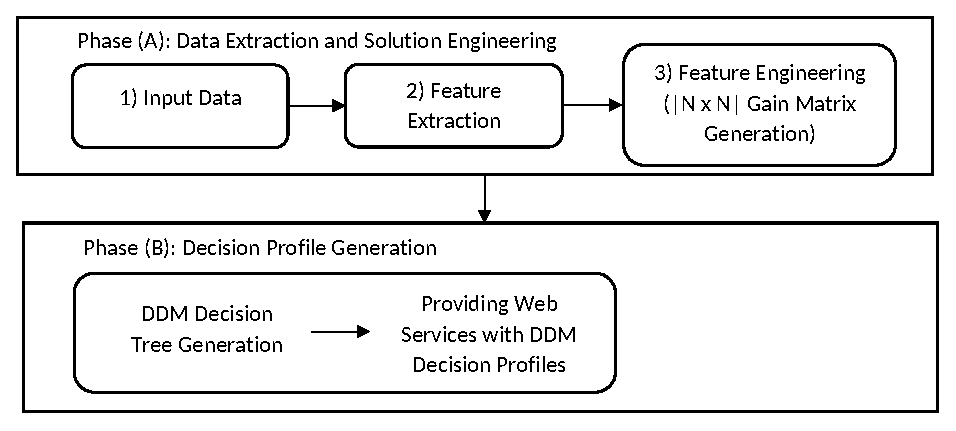
\includegraphics[width=5.25in]{figures/steps.eps}}
\caption{A summary of DDM decision profile generation steps}
\label{fig_steps}
\end{figure}

\subsection{Data Extraction and Solution Engineering}\label{ss:learningdata}

\subsubsection{Input Web Services Data}\label{sss:webservices}

%We used a data set extracted from running web services. In this data set,
Each web service is associated with a number of quality metrics that reflect its non functional parameters. These web services operate in an online environment and are continuously assigned tasks to handle. %To engage in communities, we add the external features that reflect web services' utility as a result of joining other web services to form a community (see Section \ref{s:ef}). %The additional features are %computed based on two assumptions that we adopt for a community to be formed.
We used the web services data set provided in \cite{10.1109/ISSRE.2011.17}. The raw data provides real-world QoS evaluation results from several users on 5,825 web services over 64 different time frames\footnote{http://www.wsdream.net/}. %In this data set, each web service is associated with a number of features that reflect its functionality.
%Our raw data set provides us with 64 different time slots of extracted features for each web service.
Using this data, we built a synthetic data set that contains features of a large number of web services and communities in different time intervals. The goal is to use the data set to train a decision-making model that adopts the trend of joining a community and use the model to predict/find the appropriate community for other web services. %To train our model, we build a decision tree as a benchmark for our decision making mechanism. The decision tree is made up by training the real data obtained from operating web services and extracting features related to their performance, either alone or as part of a joint effort with other web services. The ultimate objective is to propose for each web service and community the best joint decision about forming a group that maximizes every one's utility.

\subsubsection{Feature Extraction}\label{sss:filtereddata}

By processing the data provided for each web service over different time slots, we obtain the three internal quality features introduced in Section \ref{s:if}: \emph{throughput}, \emph{availability} and \emph{execution time} and the two external features discussed in Section \ref{s:ef}.  In fact, web services and communities are represented using feature vectors of these five internal and external features.

%To engage in communities, we add two additional external features that reflect web services estimation of its quality metrics compared to other web services.
%Therefore, we have generated an array of web services with three distinct features.

\begin{figure}%[!t]
\centerline{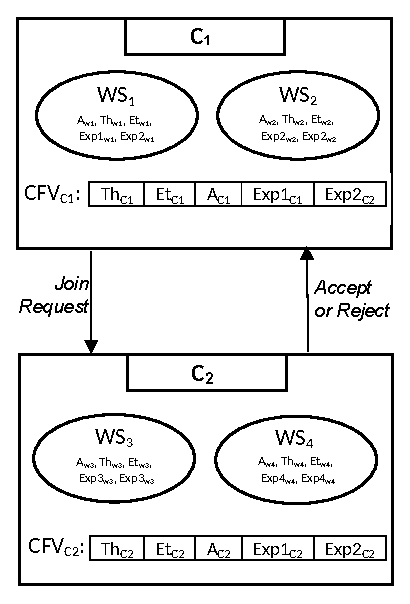
\includegraphics[width=3.15in]{figures/cfvs.eps}}
\caption{Communities with different properties of web services actively looking for other communities to collaborate with}
\label{fig_community}
\end{figure}

%By combining these three internal features to the two external features discussed in Section \ref{s:ef} that reflect the community's estimation of its quality metrics, we generate a set of feature vectors representing the communities of web services for training purposes.


We formulate a \emph{Community Feature Vector (CFV)} as $CFV_{<C>} = [f_1,...f_5]$ having a community of $k$ web services ($C = \{ws_1,...ws_k\}$, $k \geq 1$)\footnote{A web service is considered as a community of one web service.}. The features $f_1$ through $f_5$ represent the \emph{execution time}, \emph{throughput}, \emph{availability} and the \emph{external parameters 1 and 2} respectively. A set of communities, with their feature vectors and utilities evaluated, provides our algorithm with a raw training data set. We call this set of communities the \emph{template vector} $CS$, and the set of feature vectors associated with the \emph{template vector} is referred to as the \emph{community feature vector set (CFVS)}. Figure \ref{fig_community} depicts web services and communities looking to form new groups in order to improve their utility gain.

\subsubsection{Feature Engineering}\label{sss:feng}
Let $CFVS = \{CFV_{<C_1>}, \dots, CFV_{<C_N>}\}$ be the community feature vector set with $N$ communities. Based on the $CFVS$ set, we create an $|N \times N|$ gain matrix $gain^{t}$ for each time slot $t$. Each entry $gain_{n,m}^{t}$ corresponds to a utility gain of community $C_n$ when it joins community $C_m$. This gain is computed as follows: $gain_{n,m}^{t} = U_{C_n \cup C_m}^{t} - U_{C_{n}}^{t}$ where $U_{C_n \cup C_m}^{t}$ and $U_{C_{n}}^{t}$ are the utilities at time $t$ computed using Equation \ref{u_c_load}.  Evaluating the utility gain for all entries of the $gain^t$ matrix is a computationally heavy process when $N$, the size  of the feature vector set, is large. Therefore, this size should be chosen carefully.

\begin{table*}[ht]
\footnotesize
\caption{An example of $gain$ matrix for 3 different communities and their combinations} % title of Table
\centering % used for centering table
{\renewcommand{\arraystretch}{1.2}
\begin{tabular}{c|c c c c c c} % centered columns (4 columns)
\hline\hline %inserts double horizontal lines
 & \textless348\textgreater & \textless1934\textgreater & \textless2117\textgreater & \textless348, 1934\textgreater & \textless1934, 2117\textgreater & \textless348, 1934, 2117\textgreater \\ [0.5ex] % inserts table
%heading
\hline % inserts single horizontal line
\textless348\textgreater & - & 0.282708 & 1.027081 & 0.282708 & 18.027081 & 18.027081 \\
\textless1934\textgreater & -2.637483 & - & 6.969072 & -2.637483 & 5.509583 & 4.387725 \\
\textless2117\textgreater & 5.027081 & 2.969072 & - & 5.509583 & 2.969072 & 5.509583 \\
\textless348, 1934\textgreater & 0.0 & 0.0 & -3.851432 & - & -3.851432 & -3.851432 \\
\textless1934, 2117\textgreater & 2.969072 & 0.0 & 0.0 & 2.969072 & - & 2.969072 \\
\textless348, 1934, 2117\textgreater & 0.0 & 0.0 & 0.0 & 0.0 & 0.0 & - \\ [1ex] % [1ex] adds vertical space
\hline %inserts single line
\end{tabular}
}
\label{table:nonlin} % is used to refer this table in the text
\end{table*}

%Now, we let our set of communities in the $CFVS$ set, within $|T|$ time frame iterations, choose the the best communities to join.
Each community is provided with the corresponding row of data from the $gain^t$ matrix. Basically, $C_i$ is provided with the data in row $i$ of this matrix, which reports all the possible utility values $C_i$ can gain by joining different communities. By ordering the utility gain values of the row, each community is equipped with an ordered set of preferences over other communities it can join. We define $\geq_{i}^t$ as the preference order of community $i$ at time $t$.

Let $C_1 \geq_{i}^t C_2 \geq_{i}^t ~\dots~ C_{i-1} \geq_{i}^t C_{i+1} \geq_{i}^t ~\dots~ C_n$ be an ordered sequence of preferences for community $C_i$ at time $t$. Based on this sequence, we define $K^t(C_i, k)$ as a set of the $k$ most preferred communities of community $i$ at time $t$.
%\subsubsection{feature vector generation}\label{sss:fvg}
\begin{equation}\label{h_t_pref_top}
\begin{split}				
K^t(C_i, 0) = &\emptyset \\
K^t(C_i, k) = &\Big\{C_x | C_x \geq_{i}^t C_y ~\forall C_y \in CS ~\wedge~ C_x \neq C_y ~\wedge~ C_y \notin K^t(C_i, k-1) \Big\}				
\end{split}
\end{equation}
Based on $K^t(C_i, k)$, we define a set of communities $C_j$ for $C_i$ which are the $k$ most preferred communities for $C_i$ and $C_i$ belongs to the $k$ most preferred communities of $C_j$. This basically yields the preference in both sides.
\begin{equation}\label{l_t_top_both}
\begin{split}	
L^t(C_i,k) = \Big\{C_j | C_j \in K^t(C_i, k)~ \wedge~ C_i \in K^t(C_j, k)\Big\}
\end{split}
\end{equation}

Table \ref{table:nonlin} illustrates an example of a $gain$ matrix for 3 different communities and their combinations. Each row shows the gain the community can achieve by collaborating with other 5 communities. In this example, for community $\textless 348 \textgreater$ we have: \\
$K(\textless 348 \textgreater, 1) = \{\textless1934, 2117\textgreater\}$ and \\
$K(\textless 348 \textgreater, 2) = \{\textless1934, 2117\textgreater, \textless1934\textgreater\}$ \\
Since $\textless 348 \textgreater$ is the best preferred community of $\textless 1934, 2117 \textgreater$ and vice versa, therefore $L(\textless 348 \textgreater, 1)$ is not empty and contains the community $\textless1934, 2117\textgreater$.

Using the $gain$ matrix and the mentioned preference ordering relations, we are able to build a decision tree where the list of possible communities to join and their expected utilities are set.
% as well as the joined events that took place in different time slots.
In addition to the best choice, web services have access to other ordered choices and can look for the second best or third best if their first try is rejected by the target community. This aspect is analyzed in more detail in the following section, in which we launch experiments and investigate the effectiveness of the use of a decision tree with different decision layers in joining other communities and enhancing the overall utility.

\subsection{Decision Profile Generation}\label{ss:learningmodel}

Our goal is to create a decision making profile for each community in the
$CFVS$ set. We are creating an environment where the communities can experience the
outcomes of different strategies. The result will be a decision tree of the
feasible and utility-increasing moves over time. The root of the decision tree
represents a community in the $CFVS$ set, and the other nodes represent
the communities resulting from the parent node's action of joining them along with their feature values and
expected utility.


We let communities pick the best communities maximizing their utilities over different time frames. At time $t = 1$, we let each community in the $CFVS$ set choose the best community, which is a single community in the set $\{C_j\} = K^t(C_i, 1)$. If community $C_j$ also ranks $C_i$ to be the highest preferred community to join, meaning the set $L^t(C_i, k=1)$ is not empty, they would join each other. Having set $k = 1$ is a very strict and hardly satisfiable condition. In order to relax the requirement, we increase the value of $k$ by a rate $r$ proportional to time slot $t$: $k = 1 + |r \times t|$. On early steps of the training process, web services and communities are more strict, but as time goes on, we let them choose second and then third best options too. However, increasing $k$  increases the time complexity as well.

When communities $C_i$ and $C_j$ are in each other's top $k$ preference set, the new combined community, i.e., $C_i \cup C_j$ is added to the list of possible communities that can join others at time $t+1$. Moreover, for each community $C_i$ in our initial $CFVS$ set, we maintain a tree with the community $C_i$ as its root. Its children are all the communities that $C_i$ decided to join. As the scenario progresses over time, the merged communities may decide to join other communities. When communities $C_i$ and $C_j$ decide to join each other and create community $C_k$, the new community $C_k$ will be added as a child to both $C_i$ and $C_j$ nodes. At the end of the process, each community is utilized with a tree representing all possible combinations of communities it can join. Algorithm \ref{algo:dectree} illustrates the DDM tree creation procedure as pseudo-code.

\begin{algorithm}
\DontPrintSemicolon
\KwIn{$\langle r, gain^t_{n,n}, CFVS \rangle$ learning rate $r$, $|N \times N \times T|$ gain matrix, community feature vector}
\KwOut{A set of \emph{root} nodes of the decision trees}
$k \gets 1$\;
$nodes[N] \gets$ initialize $N$ tree nodes representing each community in CFVS\;
\For{$t \gets 1$ \textbf{to} $T$} {
	$k \gets 1 + round (r \times t)$\;
  \For{all $C_i \in CFVS$} {
	  \For{all $C_j \in L^t(C_i, k)$} {
      % The "l" before the If makes it so it does not expand to a second line
      \If{$C_i \in L^t(C_j, k)$}{
        $C_k \gets C_i \cup C_j$\;
				add $C_k$ to $CFVS$ set\;
				initiate $node_k$, representing $C_k$\;
				$nodes_i.addChild (node_k)$\;
				$nodes_j.addChild (node_k)$\;
      }
%      \Else{
%        $j \gets j + 1$\;
%      }			
		}
  }
%  $i \gets i + 1$\;
}
\Return{nodes}\;
\caption{{\sc DDM Decision Tree Algorithm}}
\label{algo:dectree}
\end{algorithm}

Having created $|n|$ trees, one per community, our communities are utilized with the different possible paths they can take to maximize their utilities. Using a distance function\footnote{See Section \ref{s:experiments} for an example of this function.}, communities and web services outside the training set can find the community that closely resembles their parameters within the $CFVS$ set. Those new communities can use the trees of the closest communities in the training set to have an estimation of the outcome of all possible joining actions they can take. By so doing, new communities can request to join the best communities which will maximize their gain. Such a request is most likely to be accepted as the decision considers the preferences and utility gain of the other side as well.

As a real scenario example from the used data set, Figure \ref{fig_tree} depicts a snapshot from a decision tree created by the DDM algorithm for a particular singleton community $C_{1273}$. This tree shows the different communities that $C_{1273}$ has experienced with during the training process. Each line shows the web services list within a community, the community's feature vector and the last value on each line is the overall gained  utility of the community.


\begin{figure}%[!t]
\centerline{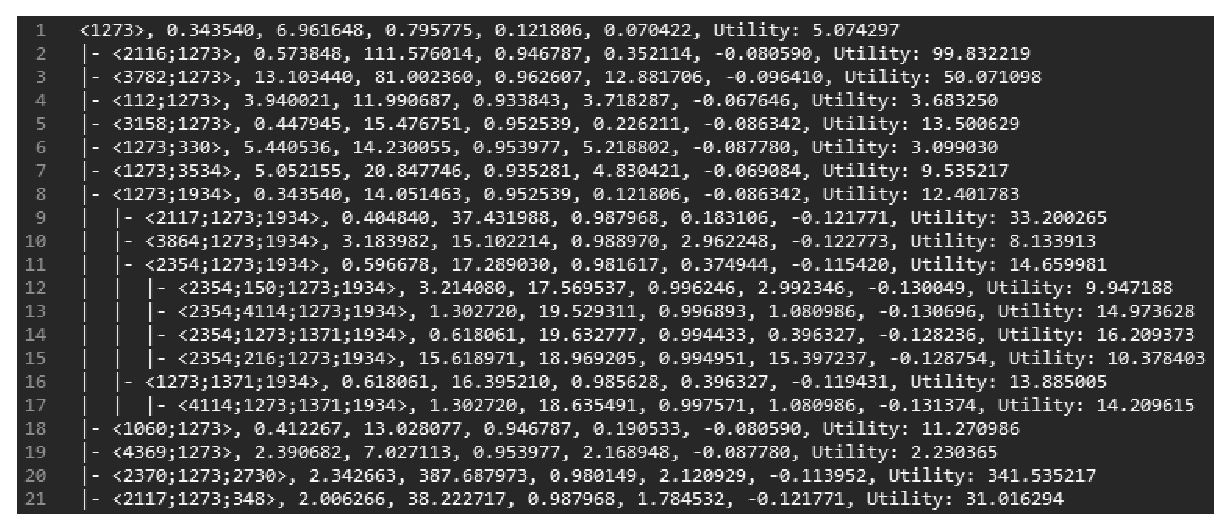
\includegraphics[width=6.25in]{figures/tree1.eps}}
\caption{A partial view of a decision tree created by DDM}
\label{fig_tree}
\end{figure}

\textbf{Complexity.} Here we analyze the computational complexity of the DDM decision tree creation algorithm on each time iteration $t$. Computing top $k$ preferred communities for $C_i$ in $K^t(C_i, k)$ requires $O(n.log(n))$ sort time. The size of $K^t(C_i, k)$ is $k$, and for each of those $k$ communities, we need to check against their $k$ top preferred communities, which needs $O(k^2)$. Line 5 iterates through $n$ communities, Line 6 takes $O(n.log(n))$ to compute and iterates $k$ times, and considering we already have the list sorted, Line 7 can reuse the sorted preferences. Thus, Line 7 takes $O(k)$ time to check if $C_i$ is member of $K^t(C_i, k)$. Multiplying these iterations, the order of complexity of the algorithm with regard to $n$ and $k$ for each time slot is: $O(k^2 \times n^2.log(n))$. Since the whole algorithm runs $T$ times, the overall complexity is $O(T \times k^2 \times n^2.log(n))$.

\section{Experiments}\label{s:experiments}
We implemented DDM in Java\footnote{Source code of implementation and data is available at: $https://github.com/Marooned202/DDM$}. We recall that we have extracted the set of features for 4532 web services in 64 different time slots through a data set provided in \cite{10.1109/ISSRE.2011.17}. By randomly choosing 86 web services out of this data set for each run, and selecting a subset of all possible combinations of sizes 2, 3, and 4 of these 86 web services, we have been able to create 10,000 communities and evaluated the feature vectors and utilities they can have in the 64 time slots. This provides us with the initial training feature set of size $|CFVS| = 10,000$ communities. Based on Equation \ref{u_c_load}, the utilities of these communities are estimated, and then the $gain$ matrix of size $|10,000 \times~ 10,000|$ of all possible ways of merging these 10,000 communities is generated\footnote {The template vector and $gain$ matrix generated are available at $https://github.com/Marooned202/DDM/tree/master/wsds/data/run$}. Based on the $gain$ matrix, each community has an ordered preference among other communities in the set.

We let communities and web services adopt their strategies based on our $DDM$ decision making mechanism. Based on the decisions adopted, each community will generate a decision tree profile. We let DDM run four times with different $r$ rates of 0.05, 0.07, 0.10 and 0.20. With the slow rate of $r = 0.05$, we increase $k$ in Equation \ref{u_c_normal} for every 20 time frames, which will happen only three times in our 64-step experiment. In the case of $r = 0.20$, $k$ increases much faster, at a rate of once every 5 time frames, which increases the complexity of the $L^t(C_i,k)$ search for each community in the $CFVS$ set.

Table \ref{table:valueandgain} depicts the average utility gain value of the communities in each of the four runs. The utility gain is the increase of utility the communities gain by cooperating and joining other communities. The utility gain ratio is the ratio of their final utility over initial utility. Comparing the different search rates, we can see that increasing the value of $r$ from $0.05$ to $0.10$ results in a significant performance boost. However, higher rates of $r$ ($r > 0.10$) are not increasing the chance of finding better collaborative groups for our communities while unnecessarily increasing the search complexity.

\begin{table}[ht]
\caption{Utility gain of web services after making collaborative groups based on DDM algorithm with different $r$ rates} % title of Table
\centering % used for centering table
{\renewcommand{\arraystretch}{1.2}
\begin{tabular}{c|c|c} % centered columns (4 columns)
\hline\hline %inserts double horizontal lines
Search Rate $r$ & Utility Gain Value & Utility Gain Ratio \\ [0.5ex] % inserts table
%heading
\hline % inserts single horizontal line
r=0.20 & 176.1499 & 6.9690 \\
r=0.10 & 174.6541 & 6.9182 \\
r=0.07 & 159.9462 & 6.2834 \\
r=0.05 & 136.0768 & 5.1032 \\ [1ex] % [1ex] adds vertical space
\hline %inserts single line
\end{tabular}
}
\label{table:valueandgain} % is used to refer this table in the text
\end{table}


%\begin{figure}%[!t]
%\centering
%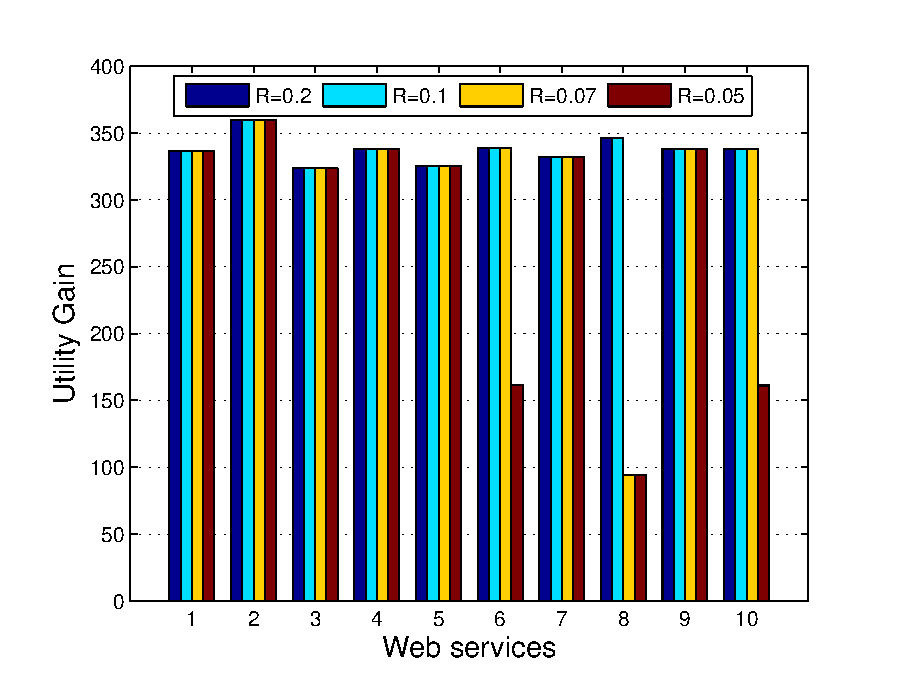
\includegraphics[width=3.5in]{figures/utility_gain_r.eps}
%\caption{DDM Utility Gain Value}
%\label{utility_gain_value}
%\end{figure}
%
%\begin{figure}%[!t]
%\centering
%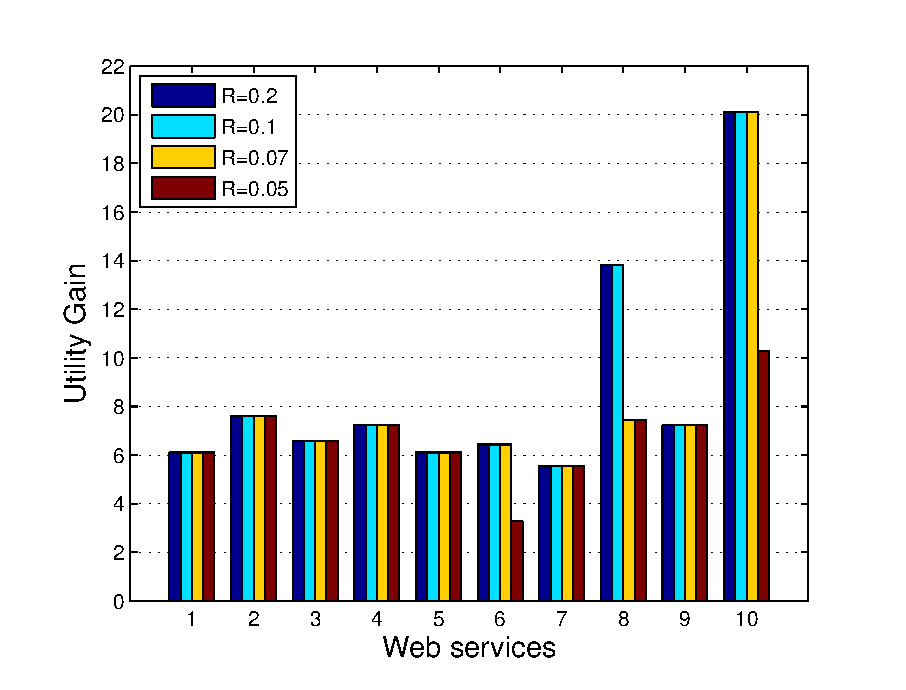
\includegraphics[width=3.5in]{figures/utility_ratio_r.eps}
%\caption{DDM Utility Gain Ratio}
%\label{utility_gain_ratio}
%\end{figure}


The closest related work \cite{10.1109/TSC.2012.12,
DBLP:conf/IEEEscc/LimTMB12, DBLP:conf/IEEEscc/KhosravifarABT11} and our
previous work \cite{journal-community-formation} regarding the community formation problem have considered a centralized approach where a community manager has complete information of all the web services and their quality
metric and parameters. Those proposals run complex algorithms through all the space of
solutions in order to find the optimal answer. However, in this paper, we
have considered an unexplored and more realistic situation where information is incomplete and a decision
profile is generated based on a smaller set of web services. Our solution helps
communities and web services select actions that lead towards
maximizing their utilities. Therefore, considering the different settings,
we cannot experimentally compare our work with the mentioned related work.


To compare our work against a benchmark, we utilize the same communities and web services with a simple rational decision making mechanism in which a community will choose to join another one if it increases its utility by any amount, without aiming to be optimal. We call this method the {\textit{rational} method. We have chosen 10 random web services and compared the results with web services which adopted our DDM model. Figure \ref{utility_gain_mlisa_and_rational} shows the comparison of the end result of utility gain values. In 18 out of 40 tries, \emph{rational} agents were not able to improve their utility at all because the communities they chose rejected their request, most likely because they would not have increased the utility of the other communities if they had joined them. The results show that a long-term strategic decision mechanism is needed to satisfy all the services within communities. Figure \ref{utility_gain_mlisa_and_rational_ratio} shows the same results in terms of ratio of utility gain.

\begin{figure}%[!t]
\centering
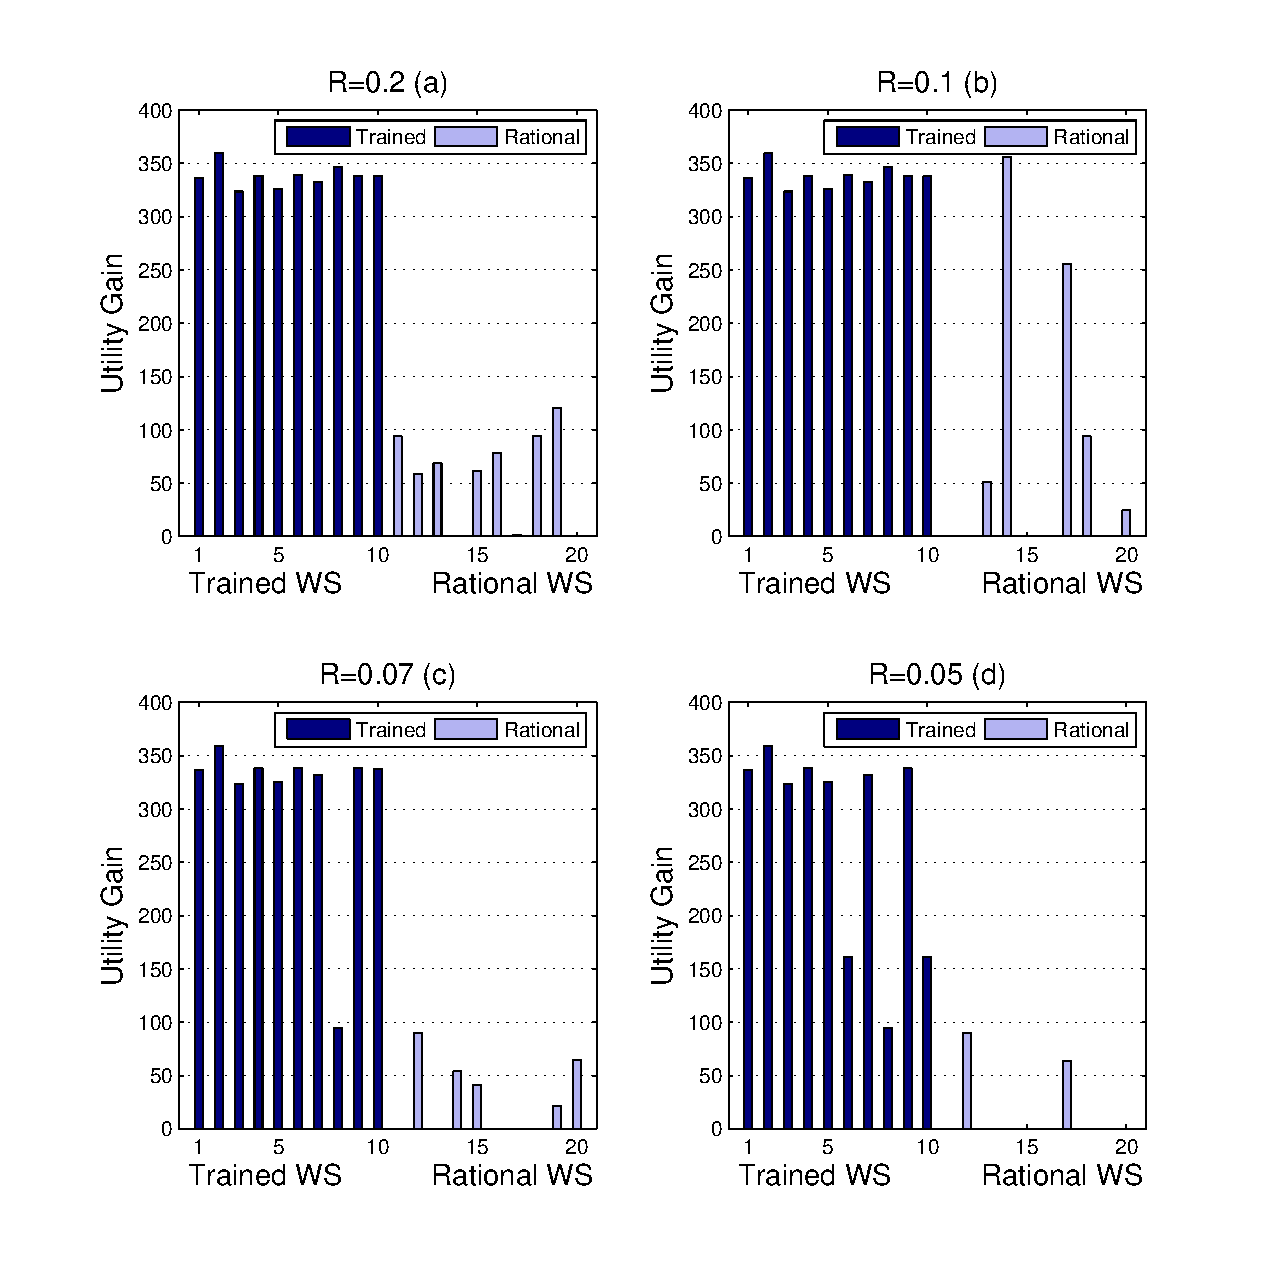
\includegraphics[width=3.5in]{figures/utility_gain.eps}
\caption{DDM against Rational: utility gain }
\label{utility_gain_mlisa_and_rational}
\end{figure}

\begin{figure}%[!t]
\centering
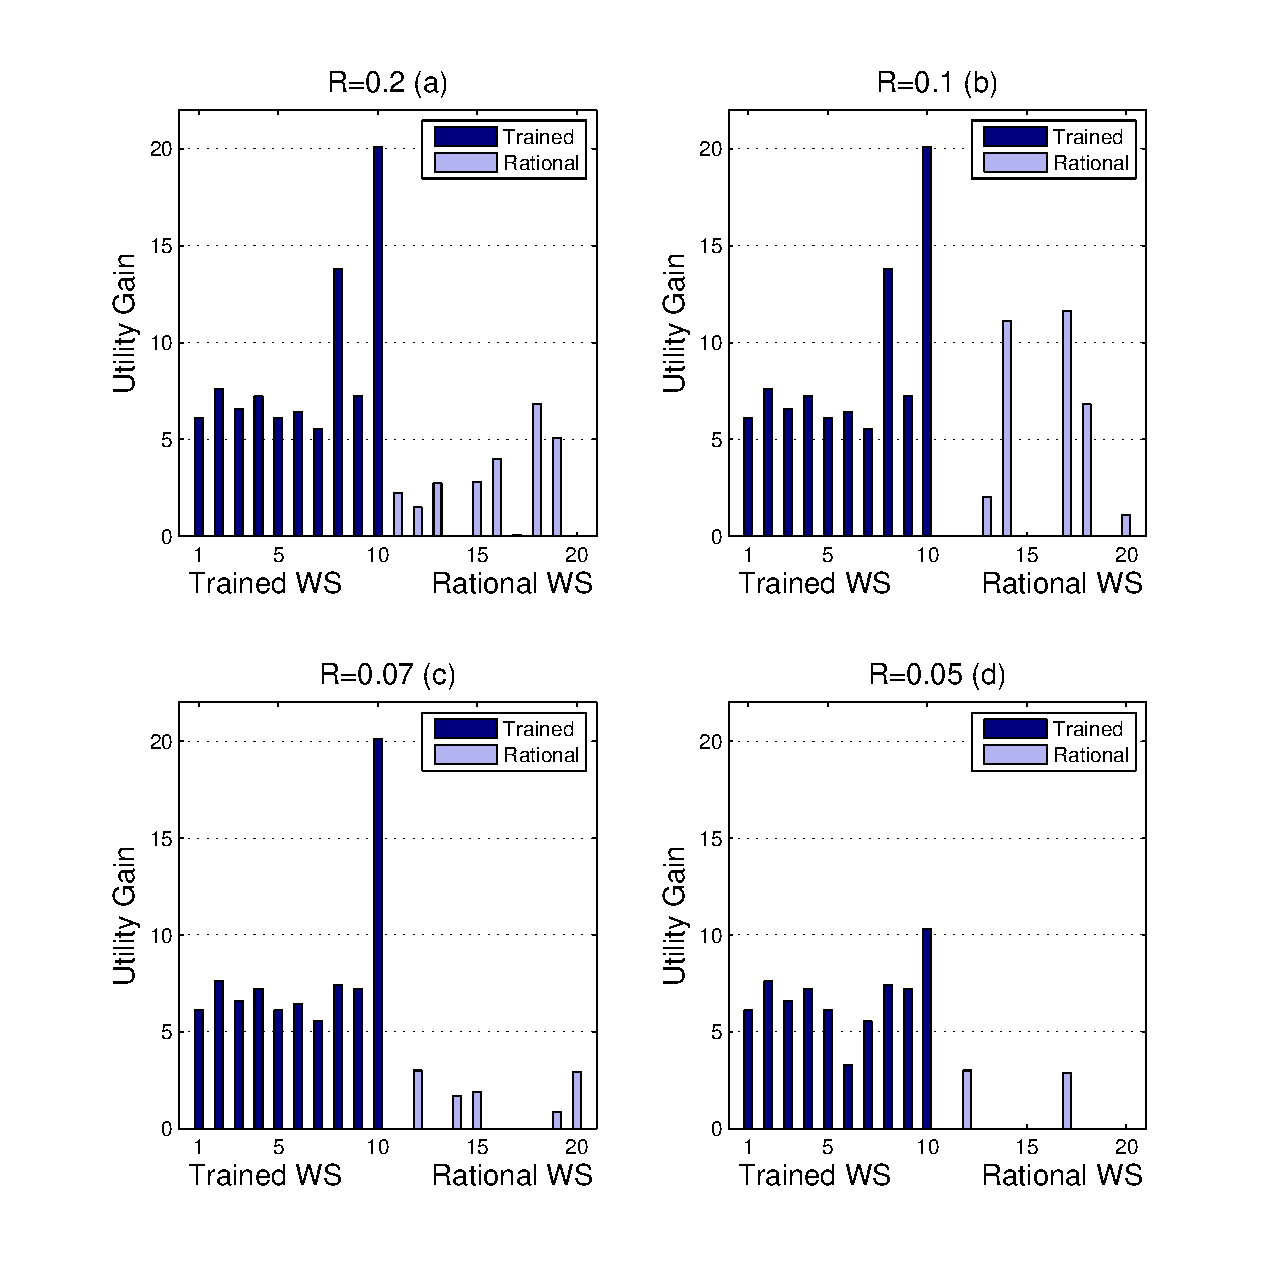
\includegraphics[width=3.5in]{figures/utility_ratio.eps}
\caption{DDM against Rational: ratio of utility gain}
\label{utility_gain_mlisa_and_rational_ratio}
\end{figure}

Now, we evaluate the performance of the decision profiles generated based on our data set for other communities.% which are not included in the decision tree creation process.
We create 1,000 communities from the web services in the data set that were not involved in the training process of our decision model. We define a distance function that measures the difference between basic features of communities, which measures the similarity among communities.

\begin{equation}\label{distance_c}
\begin{split}
distance (C_1, C_2) & = |Th_{C_1} - Th_{C_2}| \\
                    & + |A_{C_1} - A_{C_2}| + |Et_{C_1} - Et_{C_2}|
\end{split}
\end{equation}

Now, each community tries to find the closest community within the trained $CFVS$ set. Following its decision profile, the community can get a good estimate of the possible strategic decisions it can adopt. Basically, the trained profiles benefit the new communities in two ways. First, they provide the communities with a set of viable communities to join. Second, they provide an estimation of long-term utility gain for each available decision. In this experiment, we let communities follow the best decision within the decision tree provided to them.


In order to evaluate the performance of the mechanism, we used \emph{Receiver Operating Characteristic (ROC) curve}, which is a graphical plot illustrating the true negative rate against the false positive rate at various threshold settings in classifier systems. In order to classify our communities' selection strategies correctly, for each community, we evaluated the training process by replacing the community in the set with the closest one, from which it gets the strategy profile. If the actions are the same and the same utility levels are gained, we classify the decision as correct. Otherwise, it is classified as a wrong decision. \emph{AUC}, the area under the \emph{ROC curve}, is equal to the probability that a classifier will rank a randomly chosen positive instance higher than a randomly chosen negative one, and the higher the number the better the solution, which reflects better performance.  Figure \ref{roc5} illustrates the \emph{ROC curve} evaluation of the DDM decision making mechanism. As benchmark, we compare our method with two other methods: the \emph{rational} method and the \emph{greedy} method. The \emph{greedy} method only looks up the available list of communities and simply joins the community that maximizes its utility without considering any long-term strategy or other communities' acceptance scenarios. It is a greedy algorithm that focuses on choosing a locally optimal choice.

\begin{itemize}
  \item {\bf Rational Method:} Communities would send a join request to any available community, which will increase the utility. The other community would accept the join offer if its own utility gain is positive as well.
	\item {\bf Greedy Method:} Communities do a linear search among all the available communities and send a join request to the community which results in maximum utility. The other community would accept the join offer if its own utility gain is positive and the utility gain does not need to be the maximum for the community receiving the join request.
\end{itemize}

Figure \ref{roc5} compares the results for all the methods. The \emph{rational} and \emph{greedy} methods have very high failure rates compared to our method. Table \ref{fail_rate} illustrates the number of communities that failed to find the optimal collaboration group. The results support the need for a long-term training model in a successful decision making process.

\begin{figure}%[!t]
\centering
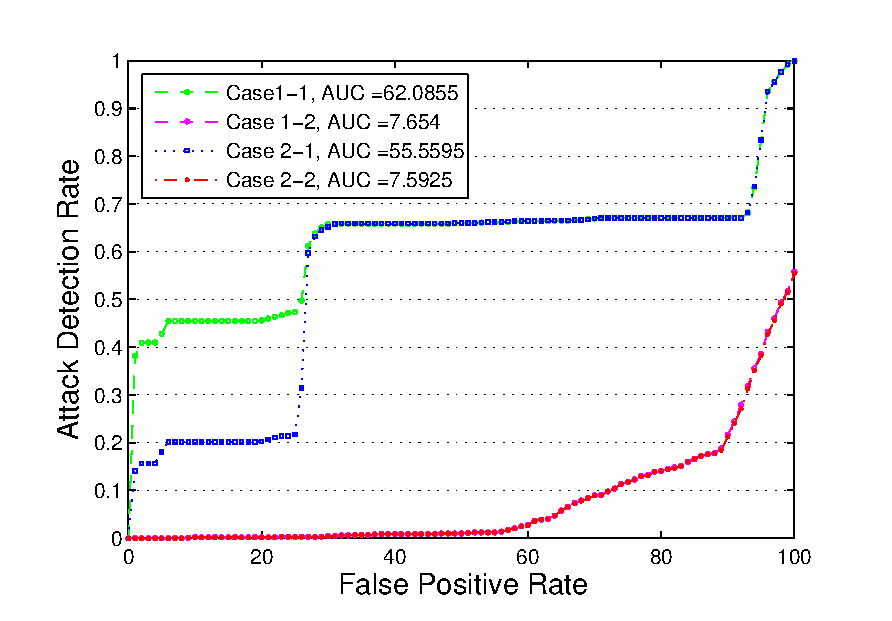
\includegraphics[width=3.5in]{figures/roc.eps}
\caption{RoC Curve}
\label{roc5}
\end{figure}

\begin{table}[ht]
\caption{Number of communities that misses the optimal decision, out of 1,000 communities} % title of Table
\centering % used for centering table
\begin{tabular}{|c|c|} % centered columns (4 columns)
\hline %inserts double horizontal lines
 Method&Miss \\ [0.5ex] % inserts table
%heading
\hline % inserts single horizontal line
 DDM r=0.05& 375 \\ % inserting body of the table
 DDM r=0.07& 137 \\
 DDM r=0.10& 6 \\
 DDM r=0.20& 6 \\
Rational Method& 717 \\
Greedy Method& 828 \\ [1ex] % [1ex] adds vertical space
\hline %inserts single line
\end{tabular}
\label{fail_rate} % is used to refer this table in the text
\end{table}


Now, we evaluate the system-specific results from users' and communities' perspectives. By distributing tasks among the communities over the 64 time frames, we evaluate the revenue for each community. Figure \ref{stats1} shows the overall revenue gain of communities using our method. Figure \ref{stats2} shows the momentarily revenue gain for each community in each time slot compared to the previous time. These results show that the run with the higher learning rate of $r=0.20$ starts discovering better communities to join much earlier. The runs with slow rates seem to find some communities to join initially, but then they slow down until later, when they start discovering new communities to join.


\begin{figure}%[!t]
\centering
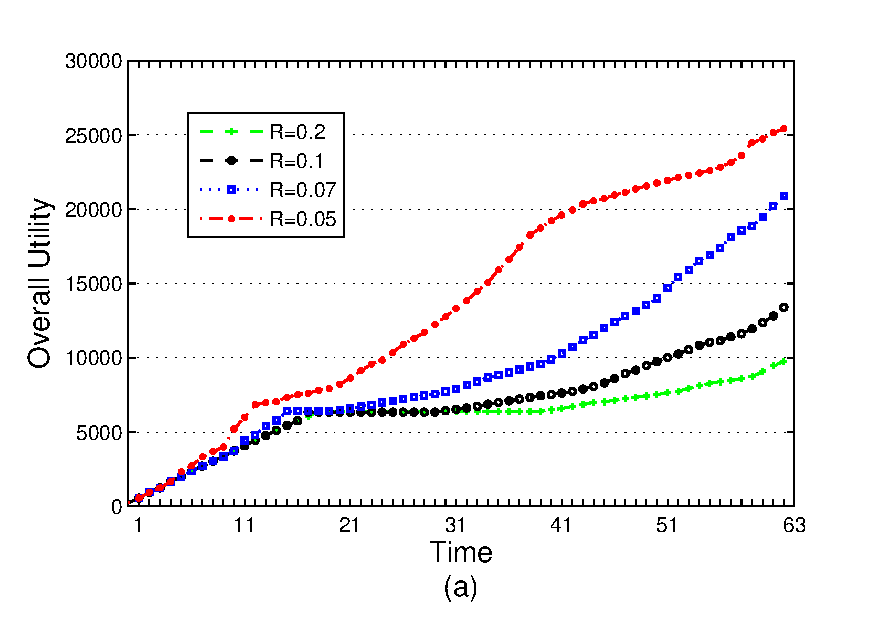
\includegraphics[width=3.5in]{figures/stats1.eps}
\caption{Overall utility of all the communities}
\label{stats1}
\end{figure}


\begin{figure}%[!t]
\centering
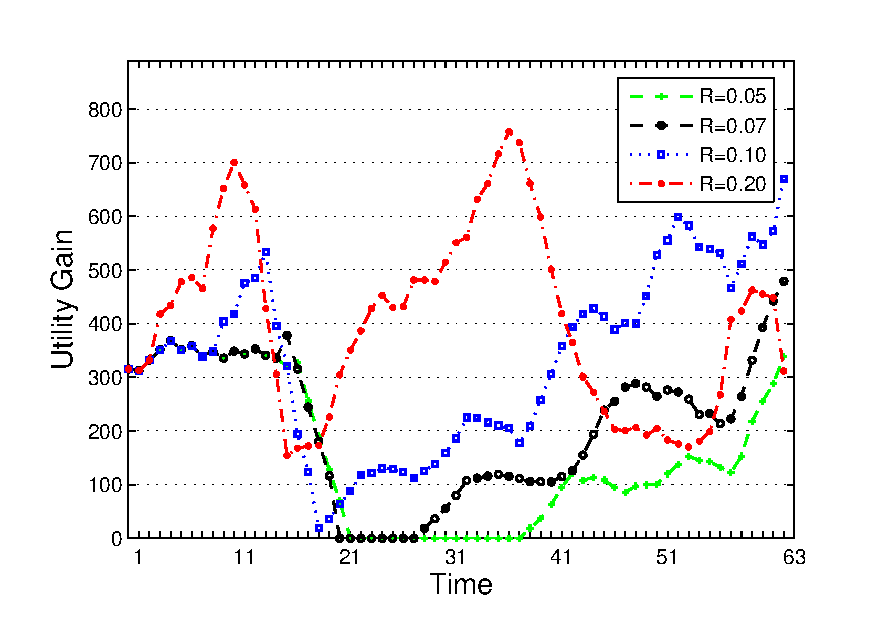
\includegraphics[width=3.5in]{figures/stats2.eps}
\caption{Utility gain over time}
\label{stats2}
\end{figure}

Figure \ref{stats3} depicts the average community size over time, which essentially represents the number of new communities being formed. The results show once again the communities using DDM with higher search rates grow faster in size, implying that the communities find appropriate web services to join with faster.

\begin{figure}%[!t]
\centering
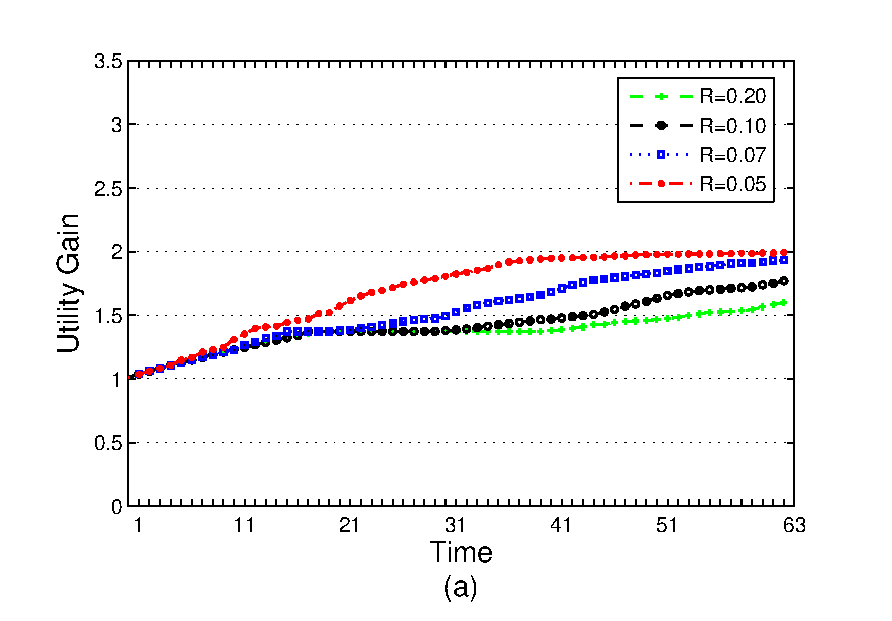
\includegraphics[width=3.5in]{figures/stats3.eps}
\caption{Average community size}
\label{stats3}
\end{figure}



\section{Related Work}\label{s:related_work}

Most of the recent work on communities of services are either
user-centric and focus on user satisfaction
\cite{Chun02user-centricperformance} or system-centric and focus
on the whole system throughput, performance and utilization. There
are many contributions in distributed, grid, cluster and cloud
services which are system-centric. However, in real world
environments and applications, both users and service providers
are self-interested agents, aiming to maximize their own profit.
In those environments, both parties (users and services) will
collaborate as long as they are getting more benefits and payoff.

In this direction, recently \cite{DBLP:conf/IEEEscc/LimTMB12,
DBLP:conf/IEEEscc/KhosravifarABT11, 10.1109/TSC.2012.12} proposed
mechanisms to help users and services maximize their gain. A
two-player non-cooperative game between web services and community
master was introduced in
\cite{DBLP:conf/IEEEscc/KhosravifarABT11}. In this game-theoretic
model, the strategies available to a web service when facing a new
community are requesting to join the community, accepting the
master's invitation to join the community, or refusing the
invitation to join. The set of strategies for communities are
inviting the web service or refusing the web service's join
request. Based on their capacity, market share and reputation, the
two players have different sets of utilities over the strategy
profiles of the game. The main limits of this game model are: 1)
its consideration of only three quality parameters, while the
other factors are simply ignored; and 2) the non-consideration of
the web services already residing within the community. The game
is only between the community master and the new web service, and
the inputs from all the other members and their influence on the
master's decision are simply ignored. The consideration of those
inputs and this influence factor is a significant issue as
existing web services can lose utility or payoff because of the
new member, which can result in an unhealthy and unstable group.
The problem comes from the fact that the existing members should
collaborate with the new web services, so probably their
performance as a group can suffer. Existing members may even
deviate and try to join other communities if they are unsatisfied.
Those considerations of forming stable and efficient coalitions
are the main contributions of our paper.

In \cite{DBLP:conf/IEEEscc/LimTMB12}, a 3-way satisfaction approach
for selecting web services has been proposed. In this approach,
the authors proposed a web service selection process that the
community masters can use. The approach considers the efficiency
of all the three involved parties, namely users, web services and
communities. In this work, it is shown how the gains of these
parties are coupled together using a linear optimization process.
However, the optimization problem in this solution tends to
optimize some parameters considering all web services regardless
of their efficiency and contribution to the community's welfare.
Moreover, there are no clear thresholds for accepting or rejecting
new web services. The solution of the optimization problem could,
for instance, suggest web services already residing within the
community to increase or decrease their capacity to cover up the
weakness of other parties in the system. However, a high
performing web service could deviate anytime it finds itself
unsatisfied within the community instead of adjusting its service
parameters.

In \cite{10.1109/TSC.2012.12}, a cooperative scheme among
autonomous web services based on coalition game theory has been
introduced. The authors have proposed an interesting algorithm to
reach individually stable coalition partition for web services in
order to maximize their efficiency. The communities choose new web
services on the promise that it would benefit the community
without decreasing any other web service's income. In the proposed
model, the worth of community is evaluated with high emphasis on
the availability metric and considering price and cost values
only. The community structure is based on a coordination chain,
where a web service is considered as a \emph{primary} web service
and the community task-distribution method initially invokes the
primary web service and only if the primary web service is
unavailable, the method invokes the next backup web services as
they are ordered in the coordination chain. We believe that this
coordination chain limits the cooperation power as it introduces a
sort of hierarchy. However, in pure and open cooperative models,
such as the one we propose in this paper, active cooperation
activities engaging simultaneously many agents so that they can
perform the tasks more efficiently are being used. Moreover, if
the availability is high, which is the case nowadays with the
recent advancements in cloud infrastructures and hardware technologies, the
backup web services will end-up having a very low chance of
getting jobs, especially the ones further in the chain. This will
results in a considerable waste of web services capabilities.

All the proposed frameworks share a common aspect, which is providing the solution based on assumption of having complete information of all services and performing evaluations based on a large number of input each time they want to adopt a strategic decision making process.
So basically, these solutions generally suffer from high complexity, which makes decision making very hard, even impossible in some cases in a real-time fashion, or they simplify important aspects to make it practical in the real world, thereby hurting the decision making performance. We address this issue by introducing DDM a framework that operates based on a trained model that regulates web service agents' decision making process in terms of cooperating with one another. After being trained, web services get to compute expectations as utilities they would gain while cooperating with communities of different characteristics. Therefore, web services and communities can make prudent decisions when inviting a web service to join or accepting a join inquiry initiated from a web service. In general, DDM equips web services with efficient methods for foreseeing how their choices will impact their long-term and short-term goals; therefore, opting for best decision available. \\

\noindent \textbf{Web Service Communities}

Here we introduce the related research work regarding the engineering and formation of communities of web services. In \cite{DBLP:journals/internet/BenatallahSD03}, Benatallah et al. defined communities of web services as \emph{Service Containers} that aggregate substitutable web services having the same set of operations and providing common functionalities. They abstracted \emph{Service Containers} as web services that are created, advertised, discovered and invoked just as elementary web services. The \emph{Container} is considered as a manager that is responsible for web service selection upon receiving a request on run-time. The authors have proposed a scoring technique based on non-functional requirements of the request and web service capabilities to dynamically chose the web service to perform the requested task. A similar concept was proposed by Maamar et al. in \cite{DBLP:journals/ijebr/MaamarSTBB09}. The authors introduced web service communities as a collection of web services with a common functionality but different QoS properties. A community manager, upon receiving a request, delegates the request to one of its current members. The choice is based on the performance history and quality metrics of each web service. The authors have proposed an efficient global web service selection algorithm in order to approach quality constraints and preferences for composite services which requires aggregation of different types of services to satisfy the user. In the same line of research, Benslimane et al. \cite{Liris-2770} have proposed a multi-layer approach grouping similar web services into communities and having an interface implemented as an abstract web service for accessing the community. The considered layers are: composite, management and community. The interactions among those layers and the bindings are performed by a generic driver called Open Software Connectivity (OSC). However, unlike our work, these proposals only tackle the problem of internal community management from the task execution perspective, but not the problem of community formation and the one of dynamically selecting which community to join and which web service to invite. Moreover, the web services selection process is done centrally by the community manager, while we address the problem more realistically from the distributed angle.

In \cite{managing-hela-jalel}, Limam and Akaichi have proposed web
service communities with centralized access across distributed web
services. They have proposed a framework for web service
management, query resolution among communities and a query caching
mechanism executed by the manager to improve the performance of
query resolution process among many distributed communities. The
key idea is to cache previous computed results for answering
future queries. Maamar et al. initially in \cite{conf/webist/MaamarLBTS07} and
then comprehensively in \cite{DBLP:journals/ijebr/MaamarSTBB09}
proposed an architecture utilizing \emph{Contract-Net} protocol
for engineering task distribution within communities of web
services. The protocol is centrally executed by the community
manager. This architecture has been further extended in
\cite{CSTintercommunity, conf/IEEEscc/BenharrefSBB11,
conf/IEEEscc/KhosravifarBMMT10, conf/aina/LimTM11}. Two types of
roles have been distinguished for community members: masters and
slaves. Master web services are community managers that lead
communities and are responsible for membership management. They
can invite and convince slave web services to join the community,
and attract new slave web services to their communities by
awarding them better payoff. Moreover, they can eject some slave
members from the community to improve its overall reputation if
these members are misbehaving or cannot provide the promised QoS.
In \cite{Medjahed05adynamic}, Medjahed and Bouguettaya have
developed a community as a ``cluster'' that groups Web services
based on a specific area of interest. All web services in a given
community share the same functionality. These communities are
created by \emph{third party community providers} which use the
\emph{community ontology} as a template and define a set of
operations that all web services within a community should
provide. Using semantic analysis on web service operations, web
services either find and join a community with similar
functionality or create a new operation description for a new
community. The authors have described the concept of
\emph{community agents} associated to \emph{community providers}.
A community agent is responsible, among other things, of the
registration of services with the community. An example of a
community that provides health care services to senior citizens
has been used. In this example, a governmental entity is needed to
check the health care standards used by the members before
authorizing them to be part of the community. Such a central
entity is represented by the community agent. Thus, community
agents are playing the role of community managers. In a close work
\cite{Zeng:2003:QDW:775152.775211}, Zeng et al. have described a
global planning selection algorithm and a delegation algorithm to
be run when a request to execute an operation is received by the
community. This needs a central entity to run those algorithms.
Such entity plays the same role as the community coordinator or
manager. All these proposals have in common the consideration
of the central entity for community management, which includes the hiring and firing of the community members, while our approach is fully distributed. Moreover, the stability of the community has not been investigated. Another major difference with our work is that the decision making process is only one way and unilateral from the community manager perspective. In our proposal, both participants, namely communities and web services, participate in the decision making process and a joining decision is made only if it is the best option for both players.


%%%%%%%%%%%%%%%%%%%%%%%%%%%%%%%%%%%%%%%%%%%%%%%%%%%%%%%%%%%%%%%
\section{Summary}\label{sec:conclusion-cha4}

In this research work, we proposed a training model for the problem of membership management of communities of web services. Using the traning model we created a decision making profile for each community and web service involved which provides them with a set of feasible and utility increasing moves. This utilized our web services with efficient methods of foreseeing how their choices of actions would impact their long-term and short-term goals, therefore they opted for best decision available. The ultimate goal is to choose the best decision when it comes to communities formation, among many possible short-term rational and utility increasing choices. The experimental results show that our algorithms provide web services and community owners, in real-world-like environments, with applicable and near-perfect decision making mechanisms. The results of experiments using real data samples support the need for a long-term training model in a successful decision making process.

Our plan for future work is to advance learning process on the training set that we provided in our work. SVN machine learning algorithm are suitable in classification of our training data set, to better classify correct or wrong decisions based on long-term utility gains, as data set outputs. This can further facilitate the process of finding optimal cooperators in regards to enhancing web services' overall performance as service providers.


%%%%%%%%%%%%%%%%%%%%%%%%%%%%%%%%%%%%%%%%%%%%%%%%%%%%%%%%%%%%%%%%%%%%%%%%%%%%%%%
%% Chapter 6 : Conclusion.
%%%%%%%%%%%%%%%%%%%%%%%%%%%%%%%%%%%%%%%%%%%%%%%%%%%%%%%%%%%%%%%%%%%%%%%%%%%%%%%
\chapter{Conclusion and Future Work}\label{Chap5:Conclusion}
%********************************************************************
%This chapter concludes the thesis. First, we give a summary of the main contributions of the thesis. Second, we present some hints for future directions.

%********************************************************************
\section{Conclusion}

In this theses we proposed three models for aggregation of web services within communities. The goal of our models are to maximize efficiency by collaborating and forming stable communities. In our first contributions we focused on stability and fairness for all web services within the communities. In this work we addressed the shortcomings of community formation in recent work such as considering best strategies which benefit all services involved, making solutions practical in real-time settings and also fairness and stability of communities. The proposed model offers an applicable mechanism for membership requests and selection of web services. The ultimate goal is to increase revenue by improving user satisfaction, which comes from the ability to perform more tasks with high quality.

In our next step of research work, we proposed DDM, a strategic distributed decision making mechanism that regulates the community formation process and membership management in communities of web services. In this work we tried to tackle the issue of autonomous web services not having a centralized architecture and complete information of all the parameters of other web services. The proposed mechanism helps web services and communities decide with whom to be grouped and cooperate. DDM first generates a trained set of data based on information obtained from large number of web services regarding their single and cooperative utilities as well as environmental parameters such as demand, service quality, etc. Communities and web services can use the trained model and instantly choose best-response strategies considering their long-term gain. In fact, the decision making mechanism is implemented as a decision tree of possible viable strategies along with their long-term expected utility. The ultimate goal of our mechanism is to choose the best decision when it comes to community formation, which goes beyond short-term utility increasing choices, usually considered in the literature. The experimental results show that our approach allows web services and communities, in real-world-like environments, to make near-perfect decisions. The results of experiments using real data samples support the need for a long-term training model in a successful decision making process.

In our final step of the work, the focus was on inter-community interaction between services involved within the community. The contribution of this model is the proposition of a coopetitive strategic model to analyze the interacting behaviour of intelligent services that are active within communities. We considered two acting strategies where service agenets expect different sort of payoffs: (1) competitive strategy where the service claims that it can accomplish a task and therefore can take the responsibility over the service consumer satisfaction; and (2) cooperative strategy where the service does not take the responsibility to accomplish the task and only cooperates with competitive peers. Our proposed model advances the state-of-the-art in cooperative systems by enabling intelligent agent-based services to effectively choose their interacting strategies that lead to optimal outcomes. The proposed framework provides a reasoning technique that service agents can use to increase their overall obtained utilities. The theoretical results presented in this thesis are also backed by simulation results using a real services dataset. Those results showed that our model outperforms existing competitive and random coopetitive strategies and the more
services deviate from the coopetitive strategy suggested by our decision-making mechanism the more they make less benefits. Thus, deviating from our coopetitive strategy yields less income for the service.


%Our plan for future work is to advance learning process on the training set that we provided in our work. SVN machine learning algorithm are suitable in classification of our training data set, to better classify correct or wrong decisions based on long-term utility gains, as data set outputs. This can further facilitate the process of finding optimal cooperators in regards to enhancing web services' overall performance as service providers.

%As future work in this area, we would like to perform more analytical and theoretical analysis on the convexity condition and also minimal $\epsilon$ values in \emph{$\epsilon$-core} solution concepts based on the characteristic function in web service applications. From web service perspective, the work can be extended to consider web service compositions where a group of web services having different set of skills cooperate to perform composite tasks. Also bargaining theory from cooperating game theory concepts can be used to help web services resolve the instability and unfairness issues by side payments.

%As future work, we plan to consider the user role in the game to obtain more accurate results when users act rationally. Moreover, we would like to achieve a collusion resistant efficiency mechanism, which is still an open problem in open environments.


\section{Future Work}

As future work, for the community formation in our first model, we would like to perform more analytical and theoretical analysis on the convexity condition and also minimal
$\epsilon$ values in \emph{$\epsilon$-core} solution concepts based on the characteristic function in web service applications. From web service perspective, the work can be extended to consider web service compositions where a group of web services having different set of skills cooperate to perform composite tasks. Also bargaining theory from cooperating game theory concepts can be used to help web services resolve the instability and unfairness issues by side payments.

For the distributed model, our future work is to advance further the learning process on the training set we provided in our work by leveraging some game theoretical approaches. In fact, game theory provides powerful techniques for strategic decision making, particularly cooperative and coalition formation games. Hedonic games and fractional hedonic games are of particular interest where the utility of a player in a community depends on the identity of the other members of the community and the value this player ascribes to those members. We intent to investigate stability solution concepts such as Shapely value so that long-term decisions will be based on the probability that the community will stay for long period. The SVM machine learning algorithm is suitable for classification of our training data set to better distinguish  decisions based on long-term utility, as data set outputs. This can further facilitate the process of finding optimal cooperators in regards to enhancing web services' overall performance as service providers.

\newpage
\textbf{Publications in refereed journals and conferences}

\textbf{Journals}

\begin{itemize}
\item E. Khosrowshahi Asl, J. Bentahar, H. Otrok, R. Mizouni, "Efficient Coalition Formation for Web Services", IEEE Transactions on Services Computing, 2015.

\item E. Khosrowshahi Asl, J. Bentahar, H. Otrok, B. Khosravifar, R. Mizouni, "To compete or cooperate? This is the question in communities of autonomous services", Journal of Expert Systems with Applications, Elsevier, 2014.

%\item F. Al-Saqqar, J. Bentahar, K. Sultan, W. Wan, E. Khosrowshahi Asl:, "Model checking temporal knowledge and commitments in multi-agent systems using reduction", Journal of Simulation Modelling Practice and Theory, 2015.

\end{itemize}

\textbf{Conferences}

\begin{itemize}
\item E. Khosrowshahi Asl, J. Bentahar, H. Otrok, R. Mizouni, "Efficient Community Formation for Web Services", IEEE SCC, Santa Clara, CA, USA, 2013.

\item B. Khoravifar, M. Alishahi, E. Khosrowshahi Asl, J. Bentahar, R. Mizouni, H. Otrok, "Analyzing Coopetition Strategies of Services within Communities", ICSOC, Shanghai, China, 2012

%\item H. O. Marey, J. Bentahar, E. Khosrowshahi Asl, M. Mbarki, R. Dssouli, "Agents' Uncertainty in Argumentation-based Negotiation: Classification and Implementation", ANT/SEIT, Hasselt, Belgium, 2014.

%\item H. Fallatah, J. Bentahar, E. Khosrowshahi Asl, "Social Network-Based Framework for Web Services Discovery", IEEE  FiCloud, Barcelona, Spain, 2014.


\end{itemize}

\textbf{Articles in process for publication in refereed journals}

\begin{itemize}
\item E. Khosrowshahi Asl, J. Bentahar, H. Otrok, R. Mizouni, "Distributed Decision Making for Dynamic Formation of Web Services Communities", Decision Support Systems, Elsevier (Submitted: June, 2015).
\end{itemize}




\typeout{------> References}
\bibliographystyle{plain}
\bibliography{ref}
%\appendix
%\input{appendix}


\end{document}


%%% Local Variables:
%%% TeX-master: t
%%% End:
